\documentclass[twoside]{book}

% Packages required by doxygen
\usepackage{fixltx2e}
\usepackage{calc}
\usepackage{doxygen}
\usepackage[export]{adjustbox} % also loads graphicx
\usepackage{graphicx}
\usepackage[utf8]{inputenc}
\usepackage{makeidx}
\usepackage{multicol}
\usepackage{multirow}
\PassOptionsToPackage{warn}{textcomp}
\usepackage{textcomp}
\usepackage[nointegrals]{wasysym}
\usepackage[table]{xcolor}

% Font selection
\usepackage[T1]{fontenc}
\usepackage[scaled=.90]{helvet}
\usepackage{courier}
\usepackage{amssymb}
\usepackage{sectsty}
\renewcommand{\familydefault}{\sfdefault}
\allsectionsfont{%
  \fontseries{bc}\selectfont%
  \color{darkgray}%
}
\renewcommand{\DoxyLabelFont}{%
  \fontseries{bc}\selectfont%
  \color{darkgray}%
}
\newcommand{\+}{\discretionary{\mbox{\scriptsize$\hookleftarrow$}}{}{}}

% Page & text layout
\usepackage{geometry}
\geometry{%
  a4paper,%
  top=2.5cm,%
  bottom=2.5cm,%
  left=2.5cm,%
  right=2.5cm%
}
\tolerance=750
\hfuzz=15pt
\hbadness=750
\setlength{\emergencystretch}{15pt}
\setlength{\parindent}{0cm}
\setlength{\parskip}{0.2cm}
\makeatletter
\renewcommand{\paragraph}{%
  \@startsection{paragraph}{4}{0ex}{-1.0ex}{1.0ex}{%
    \normalfont\normalsize\bfseries\SS@parafont%
  }%
}
\renewcommand{\subparagraph}{%
  \@startsection{subparagraph}{5}{0ex}{-1.0ex}{1.0ex}{%
    \normalfont\normalsize\bfseries\SS@subparafont%
  }%
}
\makeatother

% Headers & footers
\usepackage{fancyhdr}
\pagestyle{fancyplain}
\fancyhead[LE]{\fancyplain{}{\bfseries\thepage}}
\fancyhead[CE]{\fancyplain{}{}}
\fancyhead[RE]{\fancyplain{}{\bfseries\leftmark}}
\fancyhead[LO]{\fancyplain{}{\bfseries\rightmark}}
\fancyhead[CO]{\fancyplain{}{}}
\fancyhead[RO]{\fancyplain{}{\bfseries\thepage}}
\fancyfoot[LE]{\fancyplain{}{}}
\fancyfoot[CE]{\fancyplain{}{}}
\fancyfoot[RE]{\fancyplain{}{\bfseries\scriptsize Generated on Wed May 10 2017 14\+:54\+:09 for My Project by Doxygen }}
\fancyfoot[LO]{\fancyplain{}{\bfseries\scriptsize Generated on Wed May 10 2017 14\+:54\+:09 for My Project by Doxygen }}
\fancyfoot[CO]{\fancyplain{}{}}
\fancyfoot[RO]{\fancyplain{}{}}
\renewcommand{\footrulewidth}{0.4pt}
\renewcommand{\chaptermark}[1]{%
  \markboth{#1}{}%
}
\renewcommand{\sectionmark}[1]{%
  \markright{\thesection\ #1}%
}

% Indices & bibliography
\usepackage{natbib}
\usepackage[titles]{tocloft}
\setcounter{tocdepth}{3}
\setcounter{secnumdepth}{5}
\makeindex

% Hyperlinks (required, but should be loaded last)
\usepackage{ifpdf}
\ifpdf
  \usepackage[pdftex,pagebackref=true]{hyperref}
\else
  \usepackage[ps2pdf,pagebackref=true]{hyperref}
\fi
\hypersetup{%
  colorlinks=true,%
  linkcolor=blue,%
  citecolor=blue,%
  unicode%
}

% Custom commands
\newcommand{\clearemptydoublepage}{%
  \newpage{\pagestyle{empty}\cleardoublepage}%
}


%===== C O N T E N T S =====

\begin{document}

% Titlepage & ToC
\hypersetup{pageanchor=false,
             bookmarks=true,
             bookmarksnumbered=true,
             pdfencoding=unicode
            }
\pagenumbering{roman}
\begin{titlepage}
\vspace*{7cm}
\begin{center}%
{\Large My Project }\\
\vspace*{1cm}
{\large Generated by Doxygen 1.8.10}\\
\vspace*{0.5cm}
{\small Wed May 10 2017 14:54:09}\\
\end{center}
\end{titlepage}
\clearemptydoublepage
\tableofcontents
\clearemptydoublepage
\pagenumbering{arabic}
\hypersetup{pageanchor=true}

%--- Begin generated contents ---
\chapter{Calculator -\/ Simple object oriented software}
\label{md__read_me}
\hypertarget{md__read_me}{}
\input{md__read_me}
\chapter{Hierarchical Index}
\section{Class Hierarchy}
This inheritance list is sorted roughly, but not completely, alphabetically\+:\begin{DoxyCompactList}
\item \contentsline{section}{Calculator}{\pageref{class_calculator}}{}
\begin{DoxyCompactList}
\item \contentsline{section}{Simple\+Calculator}{\pageref{class_simple_calculator}}{}
\end{DoxyCompactList}
\item C\+Dialog\begin{DoxyCompactList}
\item \contentsline{section}{C\+About\+Dlg}{\pageref{class_c_about_dlg}}{}
\item \contentsline{section}{C\+Calculator\+Command\+Pattern\+Dlg}{\pageref{class_c_calculator_command_pattern_dlg}}{}
\end{DoxyCompactList}
\item \contentsline{section}{Command}{\pageref{class_command}}{}
\begin{DoxyCompactList}
\item \contentsline{section}{Div\+Command}{\pageref{class_div_command}}{}
\item \contentsline{section}{Eight\+Command}{\pageref{class_eight_command}}{}
\item \contentsline{section}{Enter\+Command}{\pageref{class_enter_command}}{}
\item \contentsline{section}{Five\+Command}{\pageref{class_five_command}}{}
\item \contentsline{section}{Four\+Command}{\pageref{class_four_command}}{}
\item \contentsline{section}{Minus\+Command}{\pageref{class_minus_command}}{}
\item \contentsline{section}{Mul\+Command}{\pageref{class_mul_command}}{}
\item \contentsline{section}{Nine\+Command}{\pageref{class_nine_command}}{}
\item \contentsline{section}{One\+Command}{\pageref{class_one_command}}{}
\item \contentsline{section}{Plus\+Command}{\pageref{class_plus_command}}{}
\item \contentsline{section}{Point\+Command}{\pageref{class_point_command}}{}
\item \contentsline{section}{Seven\+Command}{\pageref{class_seven_command}}{}
\item \contentsline{section}{Six\+Command}{\pageref{class_six_command}}{}
\item \contentsline{section}{Three\+Command}{\pageref{class_three_command}}{}
\item \contentsline{section}{Two\+Command}{\pageref{class_two_command}}{}
\item \contentsline{section}{Zero\+Command}{\pageref{class_zero_command}}{}
\end{DoxyCompactList}
\item \contentsline{section}{Command\+List}{\pageref{class_command_list}}{}
\item \contentsline{section}{Command\+Parser}{\pageref{class_command_parser}}{}
\begin{DoxyCompactList}
\item \contentsline{section}{Simple\+Command\+Parser}{\pageref{class_simple_command_parser}}{}
\end{DoxyCompactList}
\item C\+Win\+App\begin{DoxyCompactList}
\item \contentsline{section}{C\+Calculator\+Command\+Pattern\+App}{\pageref{class_c_calculator_command_pattern_app}}{}
\end{DoxyCompactList}
\item \contentsline{section}{Digits\+List}{\pageref{class_digits_list}}{}
\item \contentsline{section}{Invoker}{\pageref{class_invoker}}{}
\item \contentsline{section}{Math\+Op}{\pageref{class_math_op}}{}
\begin{DoxyCompactList}
\item \contentsline{section}{Div\+Math\+Op}{\pageref{class_div_math_op}}{}
\item \contentsline{section}{Minus\+Math\+Op}{\pageref{class_minus_math_op}}{}
\item \contentsline{section}{Mul\+Math\+Op}{\pageref{class_mul_math_op}}{}
\item \contentsline{section}{Plus\+Math\+Op}{\pageref{class_plus_math_op}}{}
\end{DoxyCompactList}
\item \contentsline{section}{Math\+Op\+List}{\pageref{class_math_op_list}}{}
\item \contentsline{section}{Screen}{\pageref{class_screen}}{}
\begin{DoxyCompactList}
\item \contentsline{section}{Simple\+Screen}{\pageref{class_simple_screen}}{}
\end{DoxyCompactList}
\item \contentsline{section}{Screen\+State}{\pageref{class_screen_state}}{}
\begin{DoxyCompactList}
\item \contentsline{section}{Input\+Screen\+State}{\pageref{class_input_screen_state}}{}
\item \contentsline{section}{Waiting\+Screen\+State}{\pageref{class_waiting_screen_state}}{}
\end{DoxyCompactList}
\item \contentsline{section}{Str\+To\+Dig}{\pageref{class_str_to_dig}}{}
\end{DoxyCompactList}

\chapter{Class Index}
\section{Class List}
Here are the classes, structs, unions and interfaces with brief descriptions\+:\begin{DoxyCompactList}
\item\contentsline{section}{\hyperlink{class_c_about_dlg}{C\+About\+Dlg} }{\pageref{class_c_about_dlg}}{}
\item\contentsline{section}{\hyperlink{class_c_calculator_command_pattern_app}{C\+Calculator\+Command\+Pattern\+App} }{\pageref{class_c_calculator_command_pattern_app}}{}
\item\contentsline{section}{\hyperlink{class_c_calculator_command_pattern_dlg}{C\+Calculator\+Command\+Pattern\+Dlg} }{\pageref{class_c_calculator_command_pattern_dlg}}{}
\item\contentsline{section}{\hyperlink{class_command}{Command} }{\pageref{class_command}}{}
\item\contentsline{section}{\hyperlink{class_command_list}{Command\+List} }{\pageref{class_command_list}}{}
\item\contentsline{section}{\hyperlink{class_command_parser}{Command\+Parser} \\*Abstract class  provides implementations for different types of calculations queries of commands }{\pageref{class_command_parser}}{}
\item\contentsline{section}{\hyperlink{class_digits_list}{Digits\+List} \\*Array List of doubles numbers }{\pageref{class_digits_list}}{}
\item\contentsline{section}{\hyperlink{class_div_command}{Div\+Command} \\*Implementations of dividing command }{\pageref{class_div_command}}{}
\item\contentsline{section}{\hyperlink{class_div_math_op}{Div\+Math\+Op} \\*Implentations of dividing math operation from }{\pageref{class_div_math_op}}{}
\item\contentsline{section}{\hyperlink{class_eight_command}{Eight\+Command} \\*Implementations of dividing command }{\pageref{class_eight_command}}{}
\item\contentsline{section}{\hyperlink{class_enter_command}{Enter\+Command} \\*Implementations of enter command }{\pageref{class_enter_command}}{}
\item\contentsline{section}{\hyperlink{class_five_command}{Five\+Command} \\*Implementations of five command }{\pageref{class_five_command}}{}
\item\contentsline{section}{\hyperlink{class_four_command}{Four\+Command} \\*Implementations of four command }{\pageref{class_four_command}}{}
\item\contentsline{section}{\hyperlink{class_input_screen_state}{Input\+Screen\+State} }{\pageref{class_input_screen_state}}{}
\item\contentsline{section}{\hyperlink{class_invoker}{Invoker} }{\pageref{class_invoker}}{}
\item\contentsline{section}{\hyperlink{class_math_op}{Math\+Op} }{\pageref{class_math_op}}{}
\item\contentsline{section}{\hyperlink{class_math_op_list}{Math\+Op\+List} }{\pageref{class_math_op_list}}{}
\item\contentsline{section}{\hyperlink{class_minus_command}{Minus\+Command} \\*Implementations of nine command }{\pageref{class_minus_command}}{}
\item\contentsline{section}{\hyperlink{class_minus_math_op}{Minus\+Math\+Op} }{\pageref{class_minus_math_op}}{}
\item\contentsline{section}{\hyperlink{class_mul_command}{Mul\+Command} \\*Implementations of multiply command }{\pageref{class_mul_command}}{}
\item\contentsline{section}{\hyperlink{class_mul_math_op}{Mul\+Math\+Op} }{\pageref{class_mul_math_op}}{}
\item\contentsline{section}{\hyperlink{class_nine_command}{Nine\+Command} \\*Implementations of nine command }{\pageref{class_nine_command}}{}
\item\contentsline{section}{\hyperlink{class_one_command}{One\+Command} \\*Implementations of one command }{\pageref{class_one_command}}{}
\item\contentsline{section}{\hyperlink{class_plus_command}{Plus\+Command} \\*Implementations of plus command }{\pageref{class_plus_command}}{}
\item\contentsline{section}{\hyperlink{class_plus_math_op}{Plus\+Math\+Op} }{\pageref{class_plus_math_op}}{}
\item\contentsline{section}{\hyperlink{class_point_command}{Point\+Command} \\*Implementations of dividing command }{\pageref{class_point_command}}{}
\item\contentsline{section}{\hyperlink{class_screen}{Screen} }{\pageref{class_screen}}{}
\item\contentsline{section}{\hyperlink{class_screen_state}{Screen\+State} }{\pageref{class_screen_state}}{}
\item\contentsline{section}{\hyperlink{class_seven_command}{Seven\+Command} \\*Implementations of seven command }{\pageref{class_seven_command}}{}
\item\contentsline{section}{\hyperlink{class_simple_calculator}{Simple\+Calculator} }{\pageref{class_simple_calculator}}{}
\item\contentsline{section}{\hyperlink{class_simple_command_parser}{Simple\+Command\+Parser} }{\pageref{class_simple_command_parser}}{}
\item\contentsline{section}{\hyperlink{class_simple_screen}{Simple\+Screen} }{\pageref{class_simple_screen}}{}
\item\contentsline{section}{\hyperlink{class_six_command}{Six\+Command} \\*Implementations of six command }{\pageref{class_six_command}}{}
\item\contentsline{section}{\hyperlink{class_str_to_dig}{Str\+To\+Dig} }{\pageref{class_str_to_dig}}{}
\item\contentsline{section}{\hyperlink{class_three_command}{Three\+Command} \\*Implementations of three command }{\pageref{class_three_command}}{}
\item\contentsline{section}{\hyperlink{class_two_command}{Two\+Command} \\*Implementations of two command }{\pageref{class_two_command}}{}
\item\contentsline{section}{\hyperlink{class_waiting_screen_state}{Waiting\+Screen\+State} \\*Implementations of \hyperlink{class_screen_state}{Screen\+State}. The class designed as Singletone.~\newline
 }{\pageref{class_waiting_screen_state}}{}
\item\contentsline{section}{\hyperlink{class_zero_command}{Zero\+Command} \\*Implementations of zero command }{\pageref{class_zero_command}}{}
\end{DoxyCompactList}

\chapter{Class Documentation}
\hypertarget{class_c_about_dlg}{}\section{C\+About\+Dlg Class Reference}
\label{class_c_about_dlg}\index{C\+About\+Dlg@{C\+About\+Dlg}}
Inheritance diagram for C\+About\+Dlg\+:\begin{figure}[H]
\begin{center}
\leavevmode
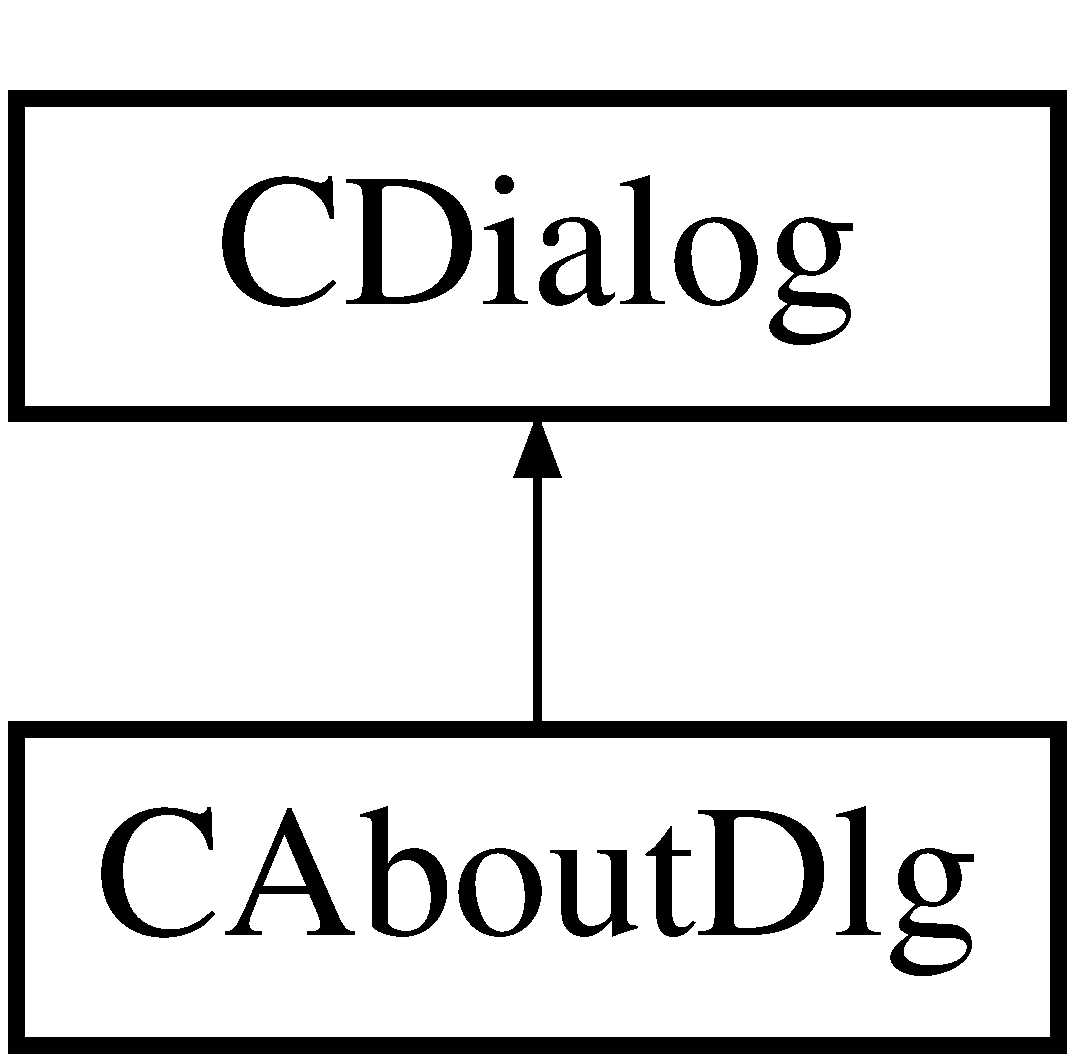
\includegraphics[height=2.000000cm]{class_c_about_dlg}
\end{center}
\end{figure}
\subsection*{Public Types}
\begin{DoxyCompactItemize}
\item 
\hypertarget{class_c_about_dlg_a27a5d4c47f16acb8562522fcd22871f7}{}enum \{ {\bfseries I\+D\+D} = I\+D\+D\+\_\+\+A\+B\+O\+U\+T\+B\+O\+X
 \}\label{class_c_about_dlg_a27a5d4c47f16acb8562522fcd22871f7}

\end{DoxyCompactItemize}
\subsection*{Protected Member Functions}
\begin{DoxyCompactItemize}
\item 
\hypertarget{class_c_about_dlg_ab83db7484fec957282d7d5a21aed4df4}{}virtual void {\bfseries Do\+Data\+Exchange} (C\+Data\+Exchange $\ast$p\+D\+X)\label{class_c_about_dlg_ab83db7484fec957282d7d5a21aed4df4}

\end{DoxyCompactItemize}


The documentation for this class was generated from the following file\+:\begin{DoxyCompactItemize}
\item 
Calculator\+Command\+Pattern\+Dlg.\+cpp\end{DoxyCompactItemize}

\hypertarget{class_calculator}{}\section{Calculator Class Reference}
\label{class_calculator}\index{Calculator@{Calculator}}
Inheritance diagram for Calculator\+:\begin{figure}[H]
\begin{center}
\leavevmode
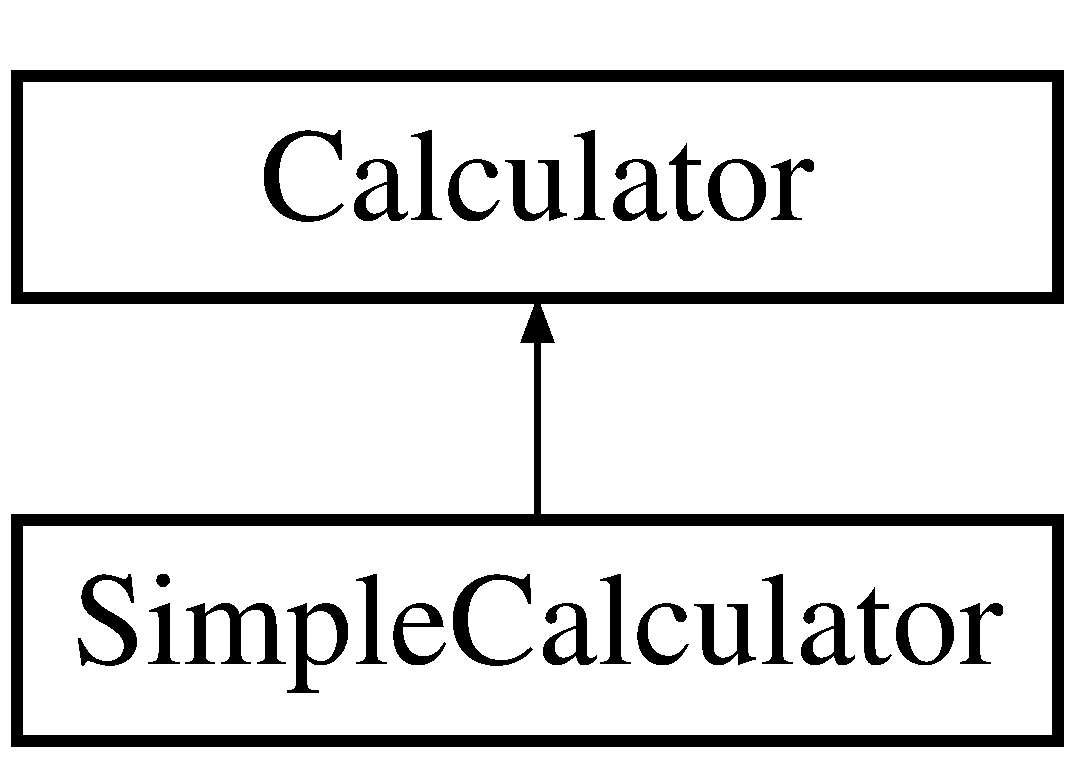
\includegraphics[height=2.000000cm]{class_calculator}
\end{center}
\end{figure}
\subsection*{Public Member Functions}
\begin{DoxyCompactItemize}
\item 
\hypertarget{class_calculator_ae4217d605a338ccc4f4cfcecaa123841}{}virtual void {\bfseries One} ()=0\label{class_calculator_ae4217d605a338ccc4f4cfcecaa123841}

\item 
\hypertarget{class_calculator_abb5d1834ef2225e15b8807327a64e2da}{}virtual void {\bfseries Two} ()=0\label{class_calculator_abb5d1834ef2225e15b8807327a64e2da}

\item 
\hypertarget{class_calculator_aaa5cbe0a2010246d0ce05016e2449ef2}{}virtual void {\bfseries Three} ()=0\label{class_calculator_aaa5cbe0a2010246d0ce05016e2449ef2}

\item 
\hypertarget{class_calculator_ac3f08818aae1d8b3224cd6de63144ae8}{}virtual void {\bfseries Four} ()=0\label{class_calculator_ac3f08818aae1d8b3224cd6de63144ae8}

\item 
\hypertarget{class_calculator_a2573d2d1ef05a81d3432358dea02ff0c}{}virtual void {\bfseries Five} ()=0\label{class_calculator_a2573d2d1ef05a81d3432358dea02ff0c}

\item 
\hypertarget{class_calculator_a4b1677e2ef25fced0c452abbbb99e169}{}virtual void {\bfseries Six} ()=0\label{class_calculator_a4b1677e2ef25fced0c452abbbb99e169}

\item 
\hypertarget{class_calculator_adacdb9d185bde6fd1ece8d8761b60d66}{}virtual void {\bfseries Seven} ()=0\label{class_calculator_adacdb9d185bde6fd1ece8d8761b60d66}

\item 
\hypertarget{class_calculator_a090ac4dd5252067aa3ad4dc1e1687fed}{}virtual void {\bfseries Eight} ()=0\label{class_calculator_a090ac4dd5252067aa3ad4dc1e1687fed}

\item 
\hypertarget{class_calculator_a2288a368de93205155380dc4abaf4169}{}virtual void {\bfseries Nine} ()=0\label{class_calculator_a2288a368de93205155380dc4abaf4169}

\item 
\hypertarget{class_calculator_a6c9b3327bc0432dc99d3e8f51d551eb1}{}virtual void {\bfseries Zero} ()=0\label{class_calculator_a6c9b3327bc0432dc99d3e8f51d551eb1}

\item 
\hypertarget{class_calculator_a40f788ae18f28acab48596c004603cff}{}virtual void {\bfseries Plus} ()=0\label{class_calculator_a40f788ae18f28acab48596c004603cff}

\item 
\hypertarget{class_calculator_a8a76dc6f06eb62fb6f38035d769f8389}{}virtual void {\bfseries Minus} ()=0\label{class_calculator_a8a76dc6f06eb62fb6f38035d769f8389}

\item 
\hypertarget{class_calculator_aa64cb3fd77df308c4d9026ca740bae54}{}virtual void {\bfseries Mul} ()=0\label{class_calculator_aa64cb3fd77df308c4d9026ca740bae54}

\item 
\hypertarget{class_calculator_aec54e6621a3751906015adcfcaadce44}{}virtual void {\bfseries Div} ()=0\label{class_calculator_aec54e6621a3751906015adcfcaadce44}

\item 
\hypertarget{class_calculator_ad0a655b502a7b7e095f00cd3eeeac492}{}virtual void {\bfseries Point} ()=0\label{class_calculator_ad0a655b502a7b7e095f00cd3eeeac492}

\item 
\hypertarget{class_calculator_a88ffe2fa664c53cfe32f4fe5b099360c}{}virtual void {\bfseries Enter} ()=0\label{class_calculator_a88ffe2fa664c53cfe32f4fe5b099360c}

\item 
\hypertarget{class_calculator_a40fad28cbf396f8bc6b479ee2a9ddf90}{}virtual void {\bfseries Undo} ()=0\label{class_calculator_a40fad28cbf396f8bc6b479ee2a9ddf90}

\item 
\hypertarget{class_calculator_a45ac4eb8a5cd868240d9fe37395b4727}{}virtual double {\bfseries get\+Result} ()=0\label{class_calculator_a45ac4eb8a5cd868240d9fe37395b4727}

\item 
\hypertarget{class_calculator_a2741fb1d13f4f12cbb3143a6f8f370ae}{}void {\bfseries set\+Command\+Parser} (\hyperlink{class_command_parser}{Command\+Parser} $\ast$new\+Command\+Parser)\label{class_calculator_a2741fb1d13f4f12cbb3143a6f8f370ae}

\item 
\hypertarget{class_calculator_acca1cf465771d79dc842b28a7575f23f}{}void {\bfseries set\+Screen} (\hyperlink{class_screen}{Screen} $\ast$new\+Screan)\label{class_calculator_acca1cf465771d79dc842b28a7575f23f}

\end{DoxyCompactItemize}
\subsection*{Public Attributes}
\begin{DoxyCompactItemize}
\item 
\hypertarget{class_calculator_a83ba050dfe21fef546e0aacf8ebb2cfb}{}\hyperlink{class_math_op_list}{Math\+Op\+List} {\bfseries math\+Ops\+List}\label{class_calculator_a83ba050dfe21fef546e0aacf8ebb2cfb}

\item 
\hypertarget{class_calculator_a4cc749b081a72aad5f5f8dbf82f95f68}{}\hyperlink{class_digits_list}{Digits\+List} {\bfseries digits\+List}\label{class_calculator_a4cc749b081a72aad5f5f8dbf82f95f68}

\item 
\hypertarget{class_calculator_a0949ffa164e30bc1993458c0c3324eae}{}\hyperlink{class_digits_list}{Digits\+List} {\bfseries result\+List}\label{class_calculator_a0949ffa164e30bc1993458c0c3324eae}

\item 
\hypertarget{class_calculator_a1b2ba1eef203f0ace18ab250b5c744e8}{}\hyperlink{class_str_to_dig}{Str\+To\+Dig} {\bfseries str\+To\+Digconv}\label{class_calculator_a1b2ba1eef203f0ace18ab250b5c744e8}

\item 
\hypertarget{class_calculator_ae2ab6e8ffe7394e5582bb0f1ed35b8aa}{}\hyperlink{class_screen}{Screen} $\ast$ {\bfseries screen}\label{class_calculator_ae2ab6e8ffe7394e5582bb0f1ed35b8aa}

\item 
\hypertarget{class_calculator_a471648b3d6fdd6773f9b6310bc94b7f1}{}\hyperlink{class_command_parser}{Command\+Parser} $\ast$ {\bfseries command\+Parser}\label{class_calculator_a471648b3d6fdd6773f9b6310bc94b7f1}

\item 
\hypertarget{class_calculator_a674f485bcc900869ed101651bebf5618}{}double {\bfseries result}\label{class_calculator_a674f485bcc900869ed101651bebf5618}

\end{DoxyCompactItemize}


The documentation for this class was generated from the following files\+:\begin{DoxyCompactItemize}
\item 
Calculator.\+h\item 
Calculator.\+cpp\end{DoxyCompactItemize}

\hypertarget{class_c_calculator_command_pattern_app}{}\section{C\+Calculator\+Command\+Pattern\+App Class Reference}
\label{class_c_calculator_command_pattern_app}\index{C\+Calculator\+Command\+Pattern\+App@{C\+Calculator\+Command\+Pattern\+App}}
Inheritance diagram for C\+Calculator\+Command\+Pattern\+App\+:\begin{figure}[H]
\begin{center}
\leavevmode
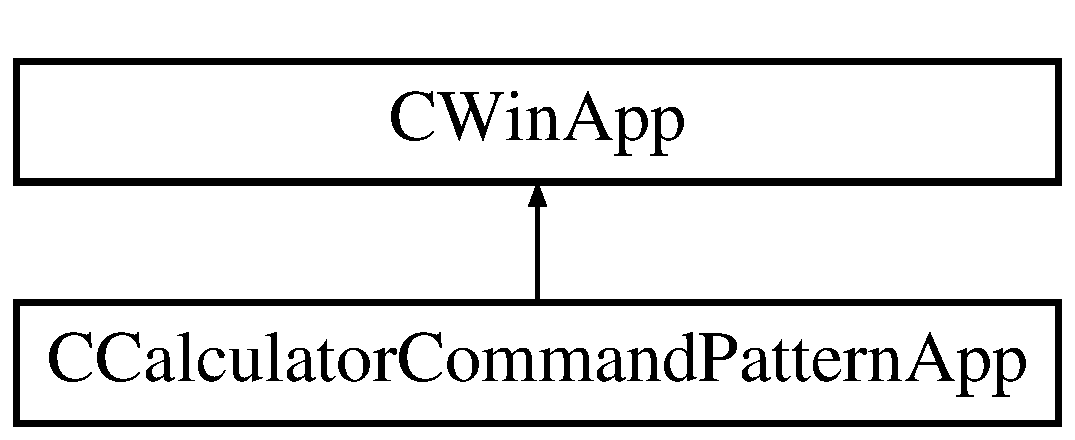
\includegraphics[height=2.000000cm]{class_c_calculator_command_pattern_app}
\end{center}
\end{figure}
\subsection*{Public Member Functions}
\begin{DoxyCompactItemize}
\item 
\hypertarget{class_c_calculator_command_pattern_app_aa7bcd7b39fd69d926dabf5d73e5f598b}{}virtual B\+O\+O\+L {\bfseries Init\+Instance} ()\label{class_c_calculator_command_pattern_app_aa7bcd7b39fd69d926dabf5d73e5f598b}

\end{DoxyCompactItemize}


The documentation for this class was generated from the following files\+:\begin{DoxyCompactItemize}
\item 
Calculator\+Command\+Pattern.\+h\item 
Calculator\+Command\+Pattern.\+cpp\end{DoxyCompactItemize}

\hypertarget{class_c_calculator_command_pattern_dlg}{}\section{C\+Calculator\+Command\+Pattern\+Dlg Class Reference}
\label{class_c_calculator_command_pattern_dlg}\index{C\+Calculator\+Command\+Pattern\+Dlg@{C\+Calculator\+Command\+Pattern\+Dlg}}
Inheritance diagram for C\+Calculator\+Command\+Pattern\+Dlg\+:\begin{figure}[H]
\begin{center}
\leavevmode
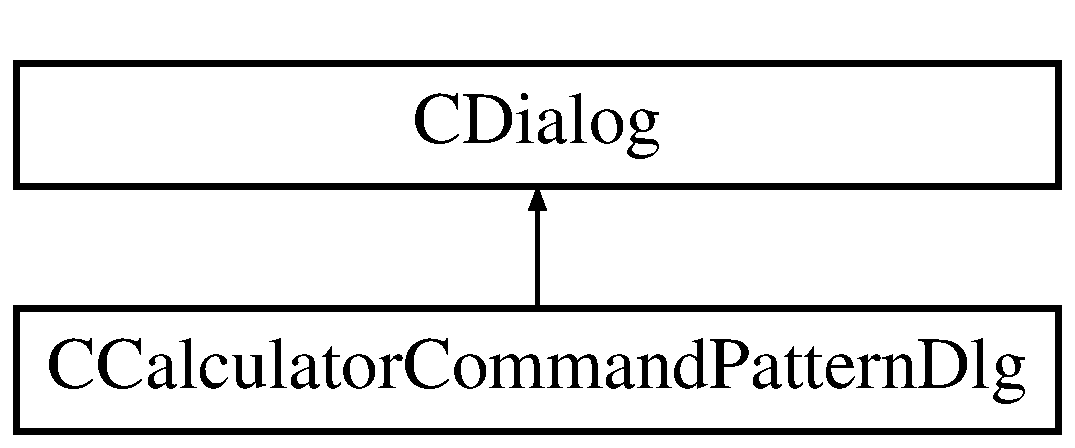
\includegraphics[height=2.000000cm]{class_c_calculator_command_pattern_dlg}
\end{center}
\end{figure}
\subsection*{Public Types}
\begin{DoxyCompactItemize}
\item 
\hypertarget{class_c_calculator_command_pattern_dlg_adb107853175bd06f53d8da3ce8888855}{}enum \{ {\bfseries I\+D\+D} = I\+D\+D\+\_\+\+C\+A\+L\+C\+U\+L\+A\+T\+O\+R\+C\+O\+M\+M\+A\+N\+D\+P\+A\+T\+T\+E\+R\+N\+\_\+\+D\+I\+A\+L\+O\+G
 \}\label{class_c_calculator_command_pattern_dlg_adb107853175bd06f53d8da3ce8888855}

\end{DoxyCompactItemize}
\subsection*{Public Member Functions}
\begin{DoxyCompactItemize}
\item 
\hypertarget{class_c_calculator_command_pattern_dlg_acbc3a8081abb686dd2a0b770d46c6a90}{}{\bfseries C\+Calculator\+Command\+Pattern\+Dlg} (C\+Wnd $\ast$p\+Parent=N\+U\+L\+L)\label{class_c_calculator_command_pattern_dlg_acbc3a8081abb686dd2a0b770d46c6a90}

\end{DoxyCompactItemize}
\subsection*{Public Attributes}
\begin{DoxyCompactItemize}
\item 
\hypertarget{class_c_calculator_command_pattern_dlg_ae03945fcd1edb609f434123010f8f815}{}C\+Button {\bfseries m\+\_\+btn\+Zero}\label{class_c_calculator_command_pattern_dlg_ae03945fcd1edb609f434123010f8f815}

\item 
\hypertarget{class_c_calculator_command_pattern_dlg_a5d9719b7524bb740e669482755430068}{}C\+Button {\bfseries m\+\_\+btn\+Two}\label{class_c_calculator_command_pattern_dlg_a5d9719b7524bb740e669482755430068}

\item 
\hypertarget{class_c_calculator_command_pattern_dlg_a08a7283ea745fee01cbe0266f689ae53}{}C\+Button {\bfseries m\+\_\+btn\+Three}\label{class_c_calculator_command_pattern_dlg_a08a7283ea745fee01cbe0266f689ae53}

\item 
\hypertarget{class_c_calculator_command_pattern_dlg_a7222996d07843143c618f78af9a28e61}{}C\+Button {\bfseries m\+\_\+btn\+Six}\label{class_c_calculator_command_pattern_dlg_a7222996d07843143c618f78af9a28e61}

\item 
\hypertarget{class_c_calculator_command_pattern_dlg_a7ae06f135d584acd2c163b8096f21e5e}{}C\+Button {\bfseries m\+\_\+btn\+Seven}\label{class_c_calculator_command_pattern_dlg_a7ae06f135d584acd2c163b8096f21e5e}

\item 
\hypertarget{class_c_calculator_command_pattern_dlg_aa178e6f59abc1e4cfb536ba364bd06ca}{}C\+Button {\bfseries m\+\_\+btn\+Plus}\label{class_c_calculator_command_pattern_dlg_aa178e6f59abc1e4cfb536ba364bd06ca}

\item 
\hypertarget{class_c_calculator_command_pattern_dlg_abd3ff0cb48f6b1c2b7e751aee38296ce}{}C\+Button {\bfseries m\+\_\+btn\+One}\label{class_c_calculator_command_pattern_dlg_abd3ff0cb48f6b1c2b7e751aee38296ce}

\item 
\hypertarget{class_c_calculator_command_pattern_dlg_a1dd33ed8814ea8310a754fd594759a18}{}C\+Button {\bfseries m\+\_\+btn\+Nine}\label{class_c_calculator_command_pattern_dlg_a1dd33ed8814ea8310a754fd594759a18}

\item 
\hypertarget{class_c_calculator_command_pattern_dlg_ac294e8f3e007def3617e0489e7782f29}{}C\+Button {\bfseries m\+\_\+btn\+Mul}\label{class_c_calculator_command_pattern_dlg_ac294e8f3e007def3617e0489e7782f29}

\item 
\hypertarget{class_c_calculator_command_pattern_dlg_af2f809977d64eeb6024ece6a822f4eb1}{}C\+Button {\bfseries m\+\_\+btn\+Minus}\label{class_c_calculator_command_pattern_dlg_af2f809977d64eeb6024ece6a822f4eb1}

\item 
\hypertarget{class_c_calculator_command_pattern_dlg_ac6ad5745f1c4831331a368cfc51c6e0d}{}C\+Button {\bfseries m\+\_\+btn\+Four}\label{class_c_calculator_command_pattern_dlg_ac6ad5745f1c4831331a368cfc51c6e0d}

\item 
\hypertarget{class_c_calculator_command_pattern_dlg_ac42d6d993f003dc5a635b5bbdbaf7ca1}{}C\+Button {\bfseries m\+\_\+btn\+Five}\label{class_c_calculator_command_pattern_dlg_ac42d6d993f003dc5a635b5bbdbaf7ca1}

\item 
\hypertarget{class_c_calculator_command_pattern_dlg_ab5d9207020d35912308daa985eed1071}{}C\+Button {\bfseries m\+\_\+btn\+Enter}\label{class_c_calculator_command_pattern_dlg_ab5d9207020d35912308daa985eed1071}

\item 
\hypertarget{class_c_calculator_command_pattern_dlg_ad365826a0dbfb5c0c4873fe3212a9720}{}C\+Button {\bfseries m\+\_\+btn\+Eight}\label{class_c_calculator_command_pattern_dlg_ad365826a0dbfb5c0c4873fe3212a9720}

\item 
\hypertarget{class_c_calculator_command_pattern_dlg_a8b64338e8ea84695318ea2bc08589215}{}C\+Button {\bfseries m\+\_\+btn\+Div}\label{class_c_calculator_command_pattern_dlg_a8b64338e8ea84695318ea2bc08589215}

\item 
\hypertarget{class_c_calculator_command_pattern_dlg_a28c25343b7c26cd1bec4892198bfdd52}{}C\+Button {\bfseries m\+\_\+btn\+Dec\+Point}\label{class_c_calculator_command_pattern_dlg_a28c25343b7c26cd1bec4892198bfdd52}

\item 
\hypertarget{class_c_calculator_command_pattern_dlg_a22610e1bb31969dd372e65070bf41a28}{}C\+Edit {\bfseries m\+\_\+ed\+Screen}\label{class_c_calculator_command_pattern_dlg_a22610e1bb31969dd372e65070bf41a28}

\end{DoxyCompactItemize}
\subsection*{Protected Member Functions}
\begin{DoxyCompactItemize}
\item 
\hypertarget{class_c_calculator_command_pattern_dlg_aa0dbbf5b84427593bed2e8465f42b0a2}{}virtual void {\bfseries Do\+Data\+Exchange} (C\+Data\+Exchange $\ast$p\+D\+X)\label{class_c_calculator_command_pattern_dlg_aa0dbbf5b84427593bed2e8465f42b0a2}

\item 
\hypertarget{class_c_calculator_command_pattern_dlg_a42f3ea55ff566dc4d720ec2ecb2a44ea}{}void {\bfseries update\+Screen} ()\label{class_c_calculator_command_pattern_dlg_a42f3ea55ff566dc4d720ec2ecb2a44ea}

\item 
\hypertarget{class_c_calculator_command_pattern_dlg_a556ebe626fa262e72863204804aec32e}{}virtual B\+O\+O\+L {\bfseries On\+Init\+Dialog} ()\label{class_c_calculator_command_pattern_dlg_a556ebe626fa262e72863204804aec32e}

\item 
\hypertarget{class_c_calculator_command_pattern_dlg_ab2ceba7c81a65e3d0bfb37ca3fec9164}{}afx\+\_\+msg void {\bfseries On\+Sys\+Command} (U\+I\+N\+T n\+I\+D, L\+P\+A\+R\+A\+M l\+Param)\label{class_c_calculator_command_pattern_dlg_ab2ceba7c81a65e3d0bfb37ca3fec9164}

\item 
\hypertarget{class_c_calculator_command_pattern_dlg_ab9c724912be2dfa09adab18aba38ce0a}{}afx\+\_\+msg void {\bfseries On\+Paint} ()\label{class_c_calculator_command_pattern_dlg_ab9c724912be2dfa09adab18aba38ce0a}

\item 
\hypertarget{class_c_calculator_command_pattern_dlg_a530286723620000fc3883cd5d1ca387d}{}afx\+\_\+msg H\+C\+U\+R\+S\+O\+R {\bfseries On\+Query\+Drag\+Icon} ()\label{class_c_calculator_command_pattern_dlg_a530286723620000fc3883cd5d1ca387d}

\item 
\hypertarget{class_c_calculator_command_pattern_dlg_a62c3ae9c25d755a160e5b6b8165b42b8}{}afx\+\_\+msg void {\bfseries On\+Zero} ()\label{class_c_calculator_command_pattern_dlg_a62c3ae9c25d755a160e5b6b8165b42b8}

\item 
\hypertarget{class_c_calculator_command_pattern_dlg_a0f8a557ec87ba8c5169b4356347e2c1b}{}afx\+\_\+msg void {\bfseries On\+One} ()\label{class_c_calculator_command_pattern_dlg_a0f8a557ec87ba8c5169b4356347e2c1b}

\item 
\hypertarget{class_c_calculator_command_pattern_dlg_a2ac26ba067fe1ef214c45f0bc0dc9782}{}afx\+\_\+msg void {\bfseries On\+Two} ()\label{class_c_calculator_command_pattern_dlg_a2ac26ba067fe1ef214c45f0bc0dc9782}

\item 
\hypertarget{class_c_calculator_command_pattern_dlg_a6fdd47ce0326b7de29875a44a0aa3bd4}{}afx\+\_\+msg void {\bfseries On\+Three} ()\label{class_c_calculator_command_pattern_dlg_a6fdd47ce0326b7de29875a44a0aa3bd4}

\item 
\hypertarget{class_c_calculator_command_pattern_dlg_ae67549929bcd27815080492b572dd192}{}afx\+\_\+msg void {\bfseries On\+Four} ()\label{class_c_calculator_command_pattern_dlg_ae67549929bcd27815080492b572dd192}

\item 
\hypertarget{class_c_calculator_command_pattern_dlg_a5b2f1cf69efbfa3afecd7ea083ad65d3}{}afx\+\_\+msg void {\bfseries On\+Five} ()\label{class_c_calculator_command_pattern_dlg_a5b2f1cf69efbfa3afecd7ea083ad65d3}

\item 
\hypertarget{class_c_calculator_command_pattern_dlg_a1164434265fe0851cfe43c45bae8abcf}{}afx\+\_\+msg void {\bfseries On\+Six} ()\label{class_c_calculator_command_pattern_dlg_a1164434265fe0851cfe43c45bae8abcf}

\item 
\hypertarget{class_c_calculator_command_pattern_dlg_a4af70eb7fbeee802f9bfaf478acaf806}{}afx\+\_\+msg void {\bfseries On\+Seven} ()\label{class_c_calculator_command_pattern_dlg_a4af70eb7fbeee802f9bfaf478acaf806}

\item 
\hypertarget{class_c_calculator_command_pattern_dlg_af726e4ca57dcdd6051d26337420c7aaa}{}afx\+\_\+msg void {\bfseries On\+Eight} ()\label{class_c_calculator_command_pattern_dlg_af726e4ca57dcdd6051d26337420c7aaa}

\item 
\hypertarget{class_c_calculator_command_pattern_dlg_a1a2c8bee2e95a5abe1719104c1ce0fe7}{}afx\+\_\+msg void {\bfseries On\+Nine} ()\label{class_c_calculator_command_pattern_dlg_a1a2c8bee2e95a5abe1719104c1ce0fe7}

\item 
\hypertarget{class_c_calculator_command_pattern_dlg_a06de33893f8d2266cd0446519566c3ba}{}afx\+\_\+msg void {\bfseries On\+Dec\+Point} ()\label{class_c_calculator_command_pattern_dlg_a06de33893f8d2266cd0446519566c3ba}

\item 
\hypertarget{class_c_calculator_command_pattern_dlg_aded22454bdde9f4f5f89b01f9cb2599d}{}afx\+\_\+msg void {\bfseries On\+Plus} ()\label{class_c_calculator_command_pattern_dlg_aded22454bdde9f4f5f89b01f9cb2599d}

\item 
\hypertarget{class_c_calculator_command_pattern_dlg_a7e2b106ae1fe1c89487ec1c45f1440c6}{}afx\+\_\+msg void {\bfseries On\+Minus} ()\label{class_c_calculator_command_pattern_dlg_a7e2b106ae1fe1c89487ec1c45f1440c6}

\item 
\hypertarget{class_c_calculator_command_pattern_dlg_afadeaa463caaa7b003d3c8b0962cfa3d}{}afx\+\_\+msg void {\bfseries On\+Mul} ()\label{class_c_calculator_command_pattern_dlg_afadeaa463caaa7b003d3c8b0962cfa3d}

\item 
\hypertarget{class_c_calculator_command_pattern_dlg_afab0bce36bdf2c8515ca51a6fffbf1ad}{}afx\+\_\+msg void {\bfseries On\+Div} ()\label{class_c_calculator_command_pattern_dlg_afab0bce36bdf2c8515ca51a6fffbf1ad}

\item 
\hypertarget{class_c_calculator_command_pattern_dlg_a134a15fa061ac0831bcc2cd1ca22a8f9}{}afx\+\_\+msg void {\bfseries On\+Enter} ()\label{class_c_calculator_command_pattern_dlg_a134a15fa061ac0831bcc2cd1ca22a8f9}

\end{DoxyCompactItemize}
\subsection*{Protected Attributes}
\begin{DoxyCompactItemize}
\item 
\hypertarget{class_c_calculator_command_pattern_dlg_a29dba11d477544ed323dd470d4d885c7}{}\hyperlink{class_invoker}{Invoker} {\bfseries invoker}\label{class_c_calculator_command_pattern_dlg_a29dba11d477544ed323dd470d4d885c7}

\item 
\hypertarget{class_c_calculator_command_pattern_dlg_a4f6f3339b71735d69e73dc4b826ba8c2}{}\hyperlink{class_simple_calculator}{Simple\+Calculator} {\bfseries calculator}\label{class_c_calculator_command_pattern_dlg_a4f6f3339b71735d69e73dc4b826ba8c2}

\item 
\hypertarget{class_c_calculator_command_pattern_dlg_af9d7533c4b711ba40d0f476b4fd61053}{}\hyperlink{class_simple_command_parser}{Simple\+Command\+Parser} {\bfseries command\+Parser}\label{class_c_calculator_command_pattern_dlg_af9d7533c4b711ba40d0f476b4fd61053}

\item 
\hypertarget{class_c_calculator_command_pattern_dlg_a6dad3f0247c1932d9ab1f16e1a509c21}{}\hyperlink{class_simple_screen}{Simple\+Screen} {\bfseries screen}\label{class_c_calculator_command_pattern_dlg_a6dad3f0247c1932d9ab1f16e1a509c21}

\item 
\hypertarget{class_c_calculator_command_pattern_dlg_a6b85b292776bfffc55649ed7029b4abb}{}H\+I\+C\+O\+N {\bfseries m\+\_\+h\+Icon}\label{class_c_calculator_command_pattern_dlg_a6b85b292776bfffc55649ed7029b4abb}

\end{DoxyCompactItemize}


The documentation for this class was generated from the following files\+:\begin{DoxyCompactItemize}
\item 
Calculator\+Command\+Pattern\+Dlg.\+h\item 
Calculator\+Command\+Pattern\+Dlg.\+cpp\end{DoxyCompactItemize}

\hypertarget{class_command}{}\section{Command Class Reference}
\label{class_command}\index{Command@{Command}}


{\ttfamily \#include $<$Command.\+h$>$}

Inheritance diagram for Command\+:\begin{figure}[H]
\begin{center}
\leavevmode
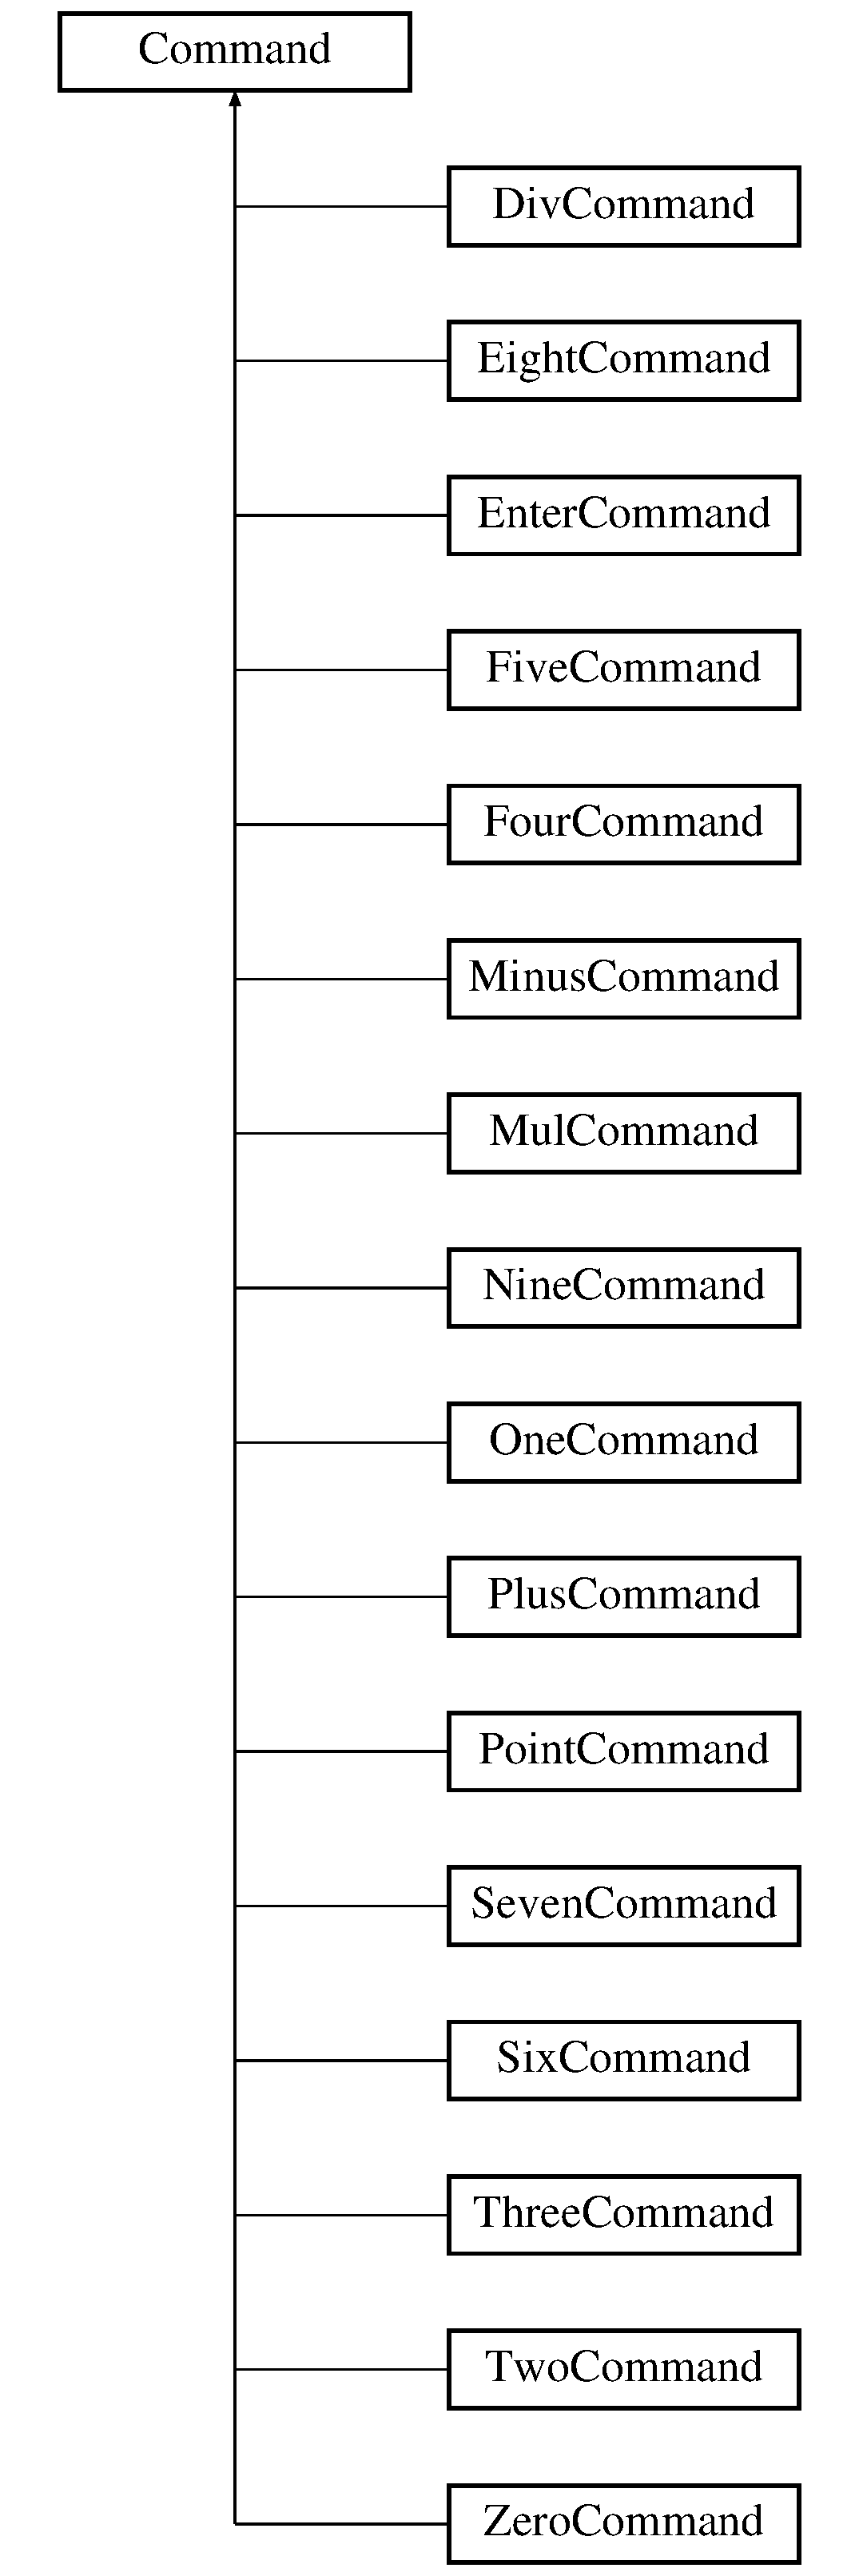
\includegraphics[height=12.000000cm]{class_command}
\end{center}
\end{figure}
\subsection*{Public Member Functions}
\begin{DoxyCompactItemize}
\item 
\hypertarget{class_command_a6fd7d9bd8df8bfc881e4d6c7cd1878b7}{}virtual void \hyperlink{class_command_a6fd7d9bd8df8bfc881e4d6c7cd1878b7}{execute} ()=0\label{class_command_a6fd7d9bd8df8bfc881e4d6c7cd1878b7}

\begin{DoxyCompactList}\small\item\em Executes some functionality in buisness logic. \end{DoxyCompactList}\end{DoxyCompactItemize}


\subsection{Detailed Description}
Abstract class command (Patern \hyperlink{class_command}{Command}). Using for connecting the interface with buisness logic 

The documentation for this class was generated from the following file\+:\begin{DoxyCompactItemize}
\item 
Command.\+h\end{DoxyCompactItemize}

\hypertarget{class_command_list}{}\section{Command\+List Class Reference}
\label{class_command_list}\index{Command\+List@{Command\+List}}
\subsection*{Public Member Functions}
\begin{DoxyCompactItemize}
\item 
\hypertarget{class_command_list_a0e24076e79f1ebe5a8cf3992873603fa}{}\hyperlink{class_command}{Command} $\ast$ {\bfseries get\+Command} ()\label{class_command_list_a0e24076e79f1ebe5a8cf3992873603fa}

\item 
\hypertarget{class_command_list_a5d11d429c550a38d9ba77ad8bc717ab9}{}\hyperlink{class_command}{Command} $\ast$ {\bfseries get\+Command} (int pos)\label{class_command_list_a5d11d429c550a38d9ba77ad8bc717ab9}

\item 
\hypertarget{class_command_list_a7faf17dcf8101bf2787ddde0e4a81353}{}void {\bfseries remove\+Command} (int pos)\label{class_command_list_a7faf17dcf8101bf2787ddde0e4a81353}

\item 
\hypertarget{class_command_list_a01627f4070f628f40b3a46bed51afc86}{}void {\bfseries add\+Command} (\hyperlink{class_command}{Command} $\ast$new\+Command)\label{class_command_list_a01627f4070f628f40b3a46bed51afc86}

\item 
\hypertarget{class_command_list_a8482ecf6e3a1c11e863fc007d6bf3365}{}bool {\bfseries has\+Next} ()\label{class_command_list_a8482ecf6e3a1c11e863fc007d6bf3365}

\item 
\hypertarget{class_command_list_a894298803e476f35ac17ab1424a11922}{}void {\bfseries set\+Head\+Pos} ()\label{class_command_list_a894298803e476f35ac17ab1424a11922}

\end{DoxyCompactItemize}
\subsection*{Public Attributes}
\begin{DoxyCompactItemize}
\item 
\hypertarget{class_command_list_adc77c49a4c604cdd32bd77ad1ee89ff6}{}int {\bfseries size}\label{class_command_list_adc77c49a4c604cdd32bd77ad1ee89ff6}

\item 
\hypertarget{class_command_list_a58ea031961578de2c50b8c0fb6f5ce31}{}int {\bfseries current\+Pos}\label{class_command_list_a58ea031961578de2c50b8c0fb6f5ce31}

\item 
\hypertarget{class_command_list_a076cd854c00450cc01218c168c01af0e}{}int {\bfseries last\+Command}\label{class_command_list_a076cd854c00450cc01218c168c01af0e}

\item 
\hypertarget{class_command_list_ae51735999a6d1f60ed22c70ae68d6482}{}\hyperlink{class_command}{Command} $\ast$$\ast$ {\bfseries commands}\label{class_command_list_ae51735999a6d1f60ed22c70ae68d6482}

\end{DoxyCompactItemize}


The documentation for this class was generated from the following files\+:\begin{DoxyCompactItemize}
\item 
Command\+List.\+h\item 
Command\+List.\+cpp\end{DoxyCompactItemize}

\hypertarget{class_command_parser}{}\section{Command\+Parser Class Reference}
\label{class_command_parser}\index{Command\+Parser@{Command\+Parser}}
Inheritance diagram for Command\+Parser\+:\begin{figure}[H]
\begin{center}
\leavevmode
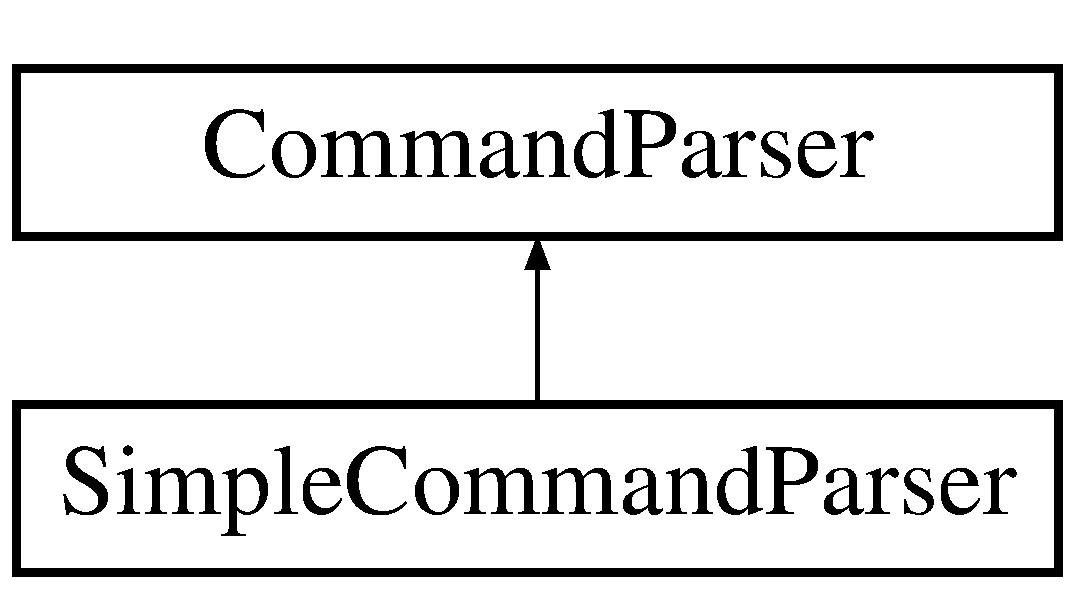
\includegraphics[height=2.000000cm]{class_command_parser}
\end{center}
\end{figure}
\subsection*{Public Member Functions}
\begin{DoxyCompactItemize}
\item 
\hypertarget{class_command_parser_a83641f98a2d06b36676af86e30974a3a}{}virtual void {\bfseries push\+Enter\+Calcul} ()=0\label{class_command_parser_a83641f98a2d06b36676af86e30974a3a}

\item 
\hypertarget{class_command_parser_a1c31dbab30dc098e1f722182030e5beb}{}virtual void {\bfseries push\+Sign\+Calcul} ()=0\label{class_command_parser_a1c31dbab30dc098e1f722182030e5beb}

\end{DoxyCompactItemize}


The documentation for this class was generated from the following file\+:\begin{DoxyCompactItemize}
\item 
Command\+Parser.\+h\end{DoxyCompactItemize}

\hypertarget{class_digits_list}{}\section{Digits\+List Class Reference}
\label{class_digits_list}\index{Digits\+List@{Digits\+List}}
\subsection*{Public Member Functions}
\begin{DoxyCompactItemize}
\item 
\hypertarget{class_digits_list_a09507db08df6c7c6013965e14f89e035}{}void {\bfseries add\+Digit} (double new\+Digit)\label{class_digits_list_a09507db08df6c7c6013965e14f89e035}

\item 
\hypertarget{class_digits_list_a28fd1ee834c98ed64dbcafe18f710e9d}{}void {\bfseries remove\+Digit} (int pos)\label{class_digits_list_a28fd1ee834c98ed64dbcafe18f710e9d}

\item 
\hypertarget{class_digits_list_ae53ff58f37f8bf8fde9ef53ab2c6c502}{}void {\bfseries set\+Haed\+Pos} ()\label{class_digits_list_ae53ff58f37f8bf8fde9ef53ab2c6c502}

\item 
\hypertarget{class_digits_list_a0494cb6bf482dbdfb45450e0ed9d3261}{}bool {\bfseries has\+Next} ()\label{class_digits_list_a0494cb6bf482dbdfb45450e0ed9d3261}

\item 
\hypertarget{class_digits_list_a41466643c41254be527aa5f17d1989bd}{}double {\bfseries get\+Last} ()\label{class_digits_list_a41466643c41254be527aa5f17d1989bd}

\item 
\hypertarget{class_digits_list_a36af51d541c102211cd7074b3d16c5f6}{}int {\bfseries get\+Last\+Pos} ()\label{class_digits_list_a36af51d541c102211cd7074b3d16c5f6}

\item 
\hypertarget{class_digits_list_a17be0b253cd525d4eff97af9d780ad72}{}double {\bfseries get} ()\label{class_digits_list_a17be0b253cd525d4eff97af9d780ad72}

\item 
\hypertarget{class_digits_list_ab9ec988cf479472b1856524c3acaf3ca}{}double {\bfseries get} (int pos)\label{class_digits_list_ab9ec988cf479472b1856524c3acaf3ca}

\end{DoxyCompactItemize}
\subsection*{Public Attributes}
\begin{DoxyCompactItemize}
\item 
\hypertarget{class_digits_list_ade233072d05a290c8dae6f76f9551831}{}double $\ast$ {\bfseries digits}\label{class_digits_list_ade233072d05a290c8dae6f76f9551831}

\item 
\hypertarget{class_digits_list_ae1e9517bd687d1b2727e84a80416b192}{}int {\bfseries size}\label{class_digits_list_ae1e9517bd687d1b2727e84a80416b192}

\item 
\hypertarget{class_digits_list_ab4978c206993f2a2f382d3f2646daded}{}int {\bfseries last\+Digit}\label{class_digits_list_ab4978c206993f2a2f382d3f2646daded}

\item 
\hypertarget{class_digits_list_a90a7daaca5877e9c9037af8449e71b68}{}int {\bfseries current\+Pos}\label{class_digits_list_a90a7daaca5877e9c9037af8449e71b68}

\end{DoxyCompactItemize}


The documentation for this class was generated from the following files\+:\begin{DoxyCompactItemize}
\item 
Digits\+List.\+h\item 
Digits\+List.\+cpp\end{DoxyCompactItemize}

\hypertarget{class_div_command}{}\section{Div\+Command Class Reference}
\label{class_div_command}\index{Div\+Command@{Div\+Command}}
Inheritance diagram for Div\+Command\+:\begin{figure}[H]
\begin{center}
\leavevmode
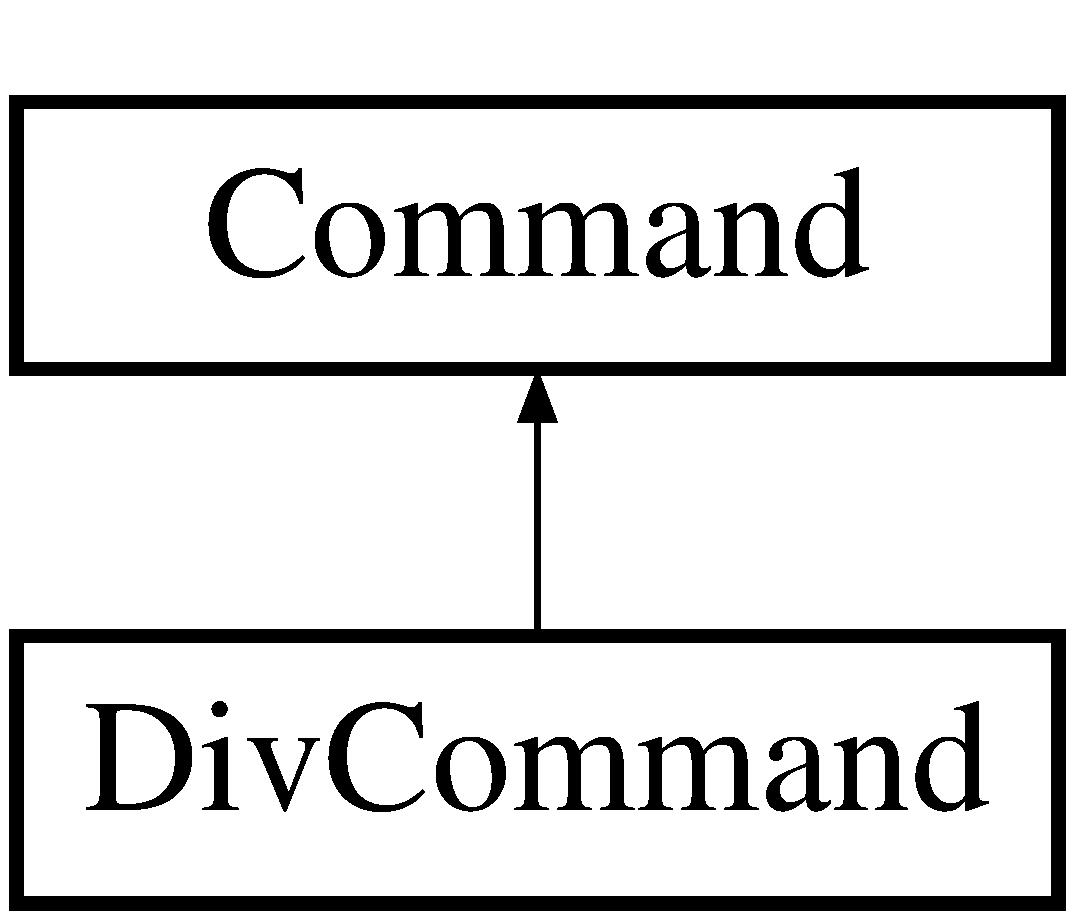
\includegraphics[height=2.000000cm]{class_div_command}
\end{center}
\end{figure}
\subsection*{Public Member Functions}
\begin{DoxyCompactItemize}
\item 
\hypertarget{class_div_command_a5e28151ba2330f4d6847723d278d2dbc}{}{\bfseries Div\+Command} (\hyperlink{class_calculator}{Calculator} $\ast$new\+Calc)\label{class_div_command_a5e28151ba2330f4d6847723d278d2dbc}

\item 
\hypertarget{class_div_command_aca34d3ac23406928629550a6d1177e0a}{}void {\bfseries execute} ()\label{class_div_command_aca34d3ac23406928629550a6d1177e0a}

\end{DoxyCompactItemize}
\subsection*{Public Attributes}
\begin{DoxyCompactItemize}
\item 
\hypertarget{class_div_command_a8773c788944f656a12c1653792abda07}{}\hyperlink{class_calculator}{Calculator} $\ast$ {\bfseries calculator}\label{class_div_command_a8773c788944f656a12c1653792abda07}

\end{DoxyCompactItemize}


The documentation for this class was generated from the following files\+:\begin{DoxyCompactItemize}
\item 
Div\+Command.\+h\item 
Div\+Command.\+cpp\end{DoxyCompactItemize}

\hypertarget{class_div_math_op}{}\section{Div\+Math\+Op Class Reference}
\label{class_div_math_op}\index{Div\+Math\+Op@{Div\+Math\+Op}}
Inheritance diagram for Div\+Math\+Op\+:\begin{figure}[H]
\begin{center}
\leavevmode
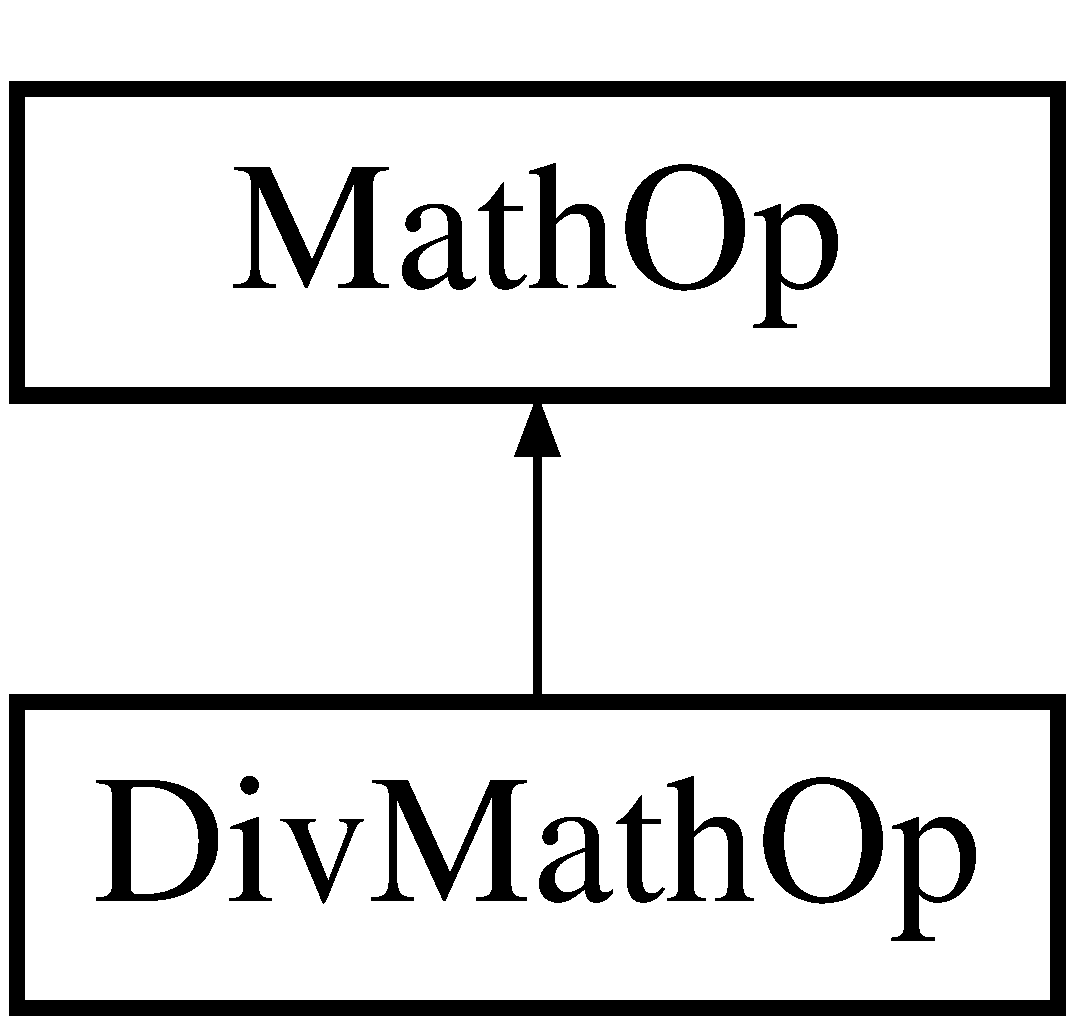
\includegraphics[height=2.000000cm]{class_div_math_op}
\end{center}
\end{figure}
\subsection*{Public Member Functions}
\begin{DoxyCompactItemize}
\item 
\hypertarget{class_div_math_op_a6055c5d403e4c33fe9ab8add65749891}{}void {\bfseries execute} ()\label{class_div_math_op_a6055c5d403e4c33fe9ab8add65749891}

\end{DoxyCompactItemize}
\subsection*{Additional Inherited Members}


The documentation for this class was generated from the following files\+:\begin{DoxyCompactItemize}
\item 
Div\+Math\+Op.\+h\item 
Div\+Math\+Op.\+cpp\end{DoxyCompactItemize}

\hypertarget{class_eight_command}{}\section{Eight\+Command Class Reference}
\label{class_eight_command}\index{Eight\+Command@{Eight\+Command}}
Inheritance diagram for Eight\+Command\+:\begin{figure}[H]
\begin{center}
\leavevmode
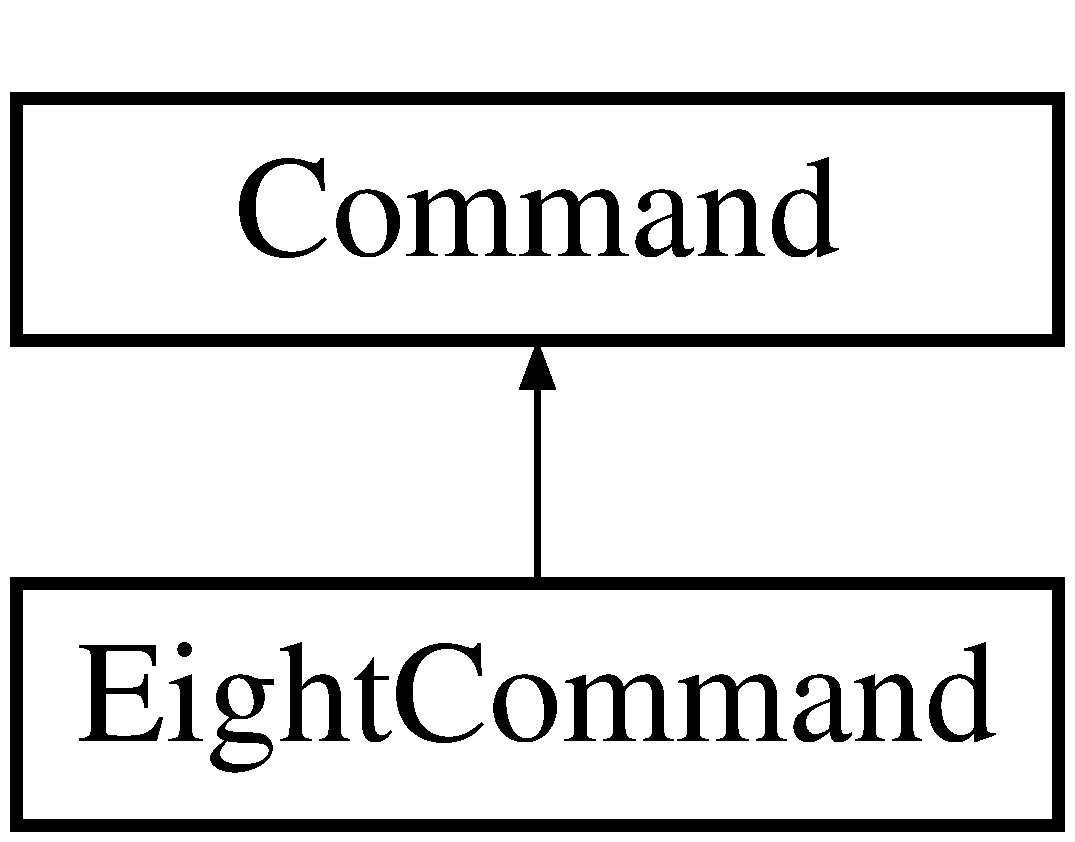
\includegraphics[height=2.000000cm]{class_eight_command}
\end{center}
\end{figure}
\subsection*{Public Member Functions}
\begin{DoxyCompactItemize}
\item 
\hypertarget{class_eight_command_afe5d23069dc3e2baa96cf239e4164023}{}{\bfseries Eight\+Command} (\hyperlink{class_calculator}{Calculator} $\ast$new\+Calc)\label{class_eight_command_afe5d23069dc3e2baa96cf239e4164023}

\item 
\hypertarget{class_eight_command_afe2b90086e76b28a9adbcde328c1b2ce}{}void \hyperlink{class_eight_command_afe2b90086e76b28a9adbcde328c1b2ce}{execute} ()\label{class_eight_command_afe2b90086e76b28a9adbcde328c1b2ce}

\begin{DoxyCompactList}\small\item\em Executes some functionality in buisness logic. \end{DoxyCompactList}\end{DoxyCompactItemize}
\subsection*{Public Attributes}
\begin{DoxyCompactItemize}
\item 
\hypertarget{class_eight_command_aa4c2a48089ca694fc1122902fc5439c0}{}\hyperlink{class_calculator}{Calculator} $\ast$ {\bfseries calculator}\label{class_eight_command_aa4c2a48089ca694fc1122902fc5439c0}

\end{DoxyCompactItemize}


The documentation for this class was generated from the following files\+:\begin{DoxyCompactItemize}
\item 
Eight\+Command.\+h\item 
Eight\+Command.\+cpp\end{DoxyCompactItemize}

\hypertarget{class_enter_command}{}\section{Enter\+Command Class Reference}
\label{class_enter_command}\index{Enter\+Command@{Enter\+Command}}


implementations of enter command  




{\ttfamily \#include $<$Enter\+Command.\+h$>$}

Inheritance diagram for Enter\+Command\+:\begin{figure}[H]
\begin{center}
\leavevmode
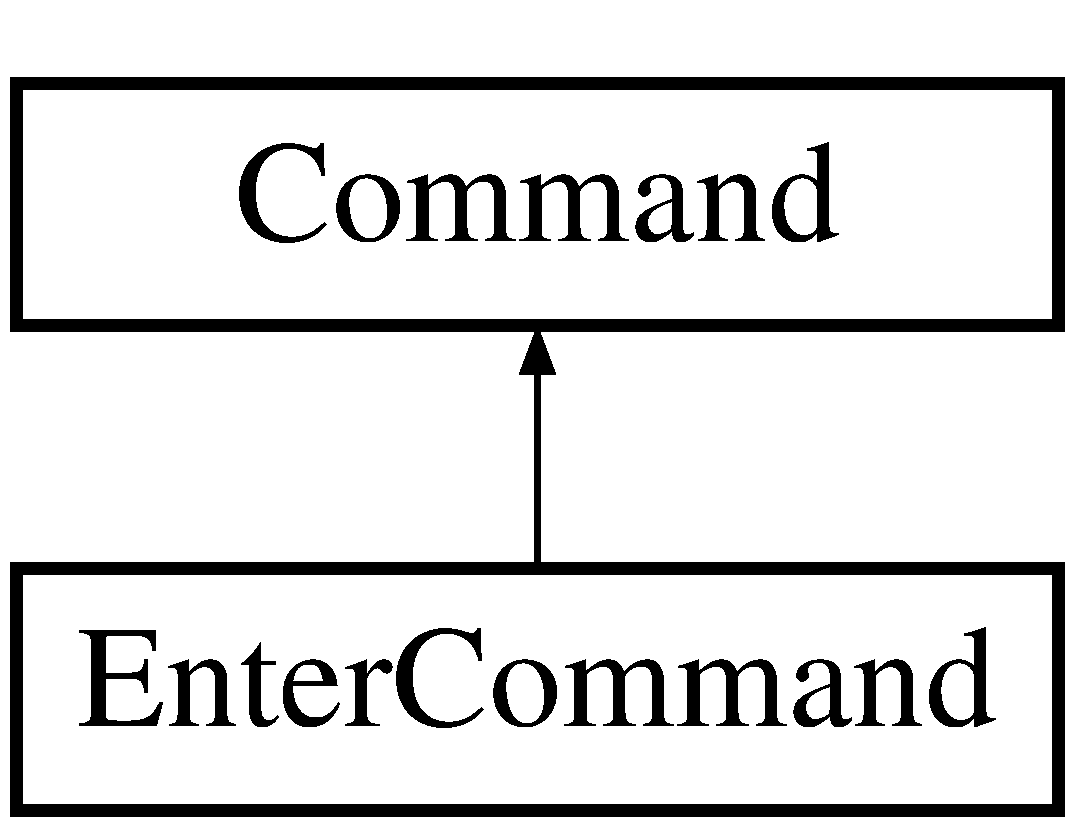
\includegraphics[height=2.000000cm]{class_enter_command}
\end{center}
\end{figure}
\subsection*{Public Member Functions}
\begin{DoxyCompactItemize}
\item 
\hyperlink{class_enter_command_aa582c411b3919835a7ff06ec5f089a66}{Enter\+Command} (Calculator $\ast$new\+Calc)
\begin{DoxyCompactList}\small\item\em A constructor. Sets pointer to the implementation of. \end{DoxyCompactList}\item 
\hyperlink{class_enter_command_a9eaab904e5bb6c0128e585cfa983b463}{$\sim$\+Enter\+Command} ()
\item 
void \hyperlink{class_enter_command_ae8701c3ea3682f566dfbcd3415a767f8}{execute} ()
\begin{DoxyCompactList}\small\item\em Executes enter command of. \end{DoxyCompactList}\end{DoxyCompactItemize}
\subsection*{Public Attributes}
\begin{DoxyCompactItemize}
\item 
Calculator $\ast$ \hyperlink{class_enter_command_a565ba3ebfd7b06dcd5fd30baa806f798}{calculator}
\end{DoxyCompactItemize}


\subsection{Detailed Description}
implementations of enter command 

Calculator -\/ Simple calculator realization by patterns Copyright (C) 2017 -\/ ? Alexey Konyshev (\href{mailto:aleksey.konyshev@gmail.com}{\tt aleksey.\+konyshev@gmail.\+com})

This software is provided \textquotesingle{}as-\/is\textquotesingle{}, without any express or implied warranty. In no event will the authors be held liable for any damages arising from the use of this software.

Permission is granted to anyone to use this software for any purpose, including commercial applications, and to alter it and redistribute it freely, subject to the following restrictions\+:


\begin{DoxyEnumerate}
\item The origin of this software must not be misrepresented; you must not claim that you wrote the original software. If you use this software in a product, an acknowledgment in the product documentation would be appreciated but is not required.
\item Altered source versions must be plainly marked as such, and must not be misrepresented as being the original software.
\item This notice may not be removed or altered from any source distribution. Headers 
\begin{DoxyCode}
\hyperlink{class_command}{Command} 
\end{DoxyCode}
 
\end{DoxyEnumerate}

\subsection{Constructor \& Destructor Documentation}
\hypertarget{class_enter_command_aa582c411b3919835a7ff06ec5f089a66}{}\index{Enter\+Command@{Enter\+Command}!Enter\+Command@{Enter\+Command}}
\index{Enter\+Command@{Enter\+Command}!Enter\+Command@{Enter\+Command}}
\subsubsection[{Enter\+Command(\+Calculator $\ast$new\+Calc)}]{\setlength{\rightskip}{0pt plus 5cm}Enter\+Command\+::\+Enter\+Command (
\begin{DoxyParamCaption}
\item[{Calculator $\ast$}]{new\+Calc}
\end{DoxyParamCaption}
)}\label{class_enter_command_aa582c411b3919835a7ff06ec5f089a66}


A constructor. Sets pointer to the implementation of. 


\begin{DoxyCode}
Calculator 
\end{DoxyCode}



\begin{DoxyParams}{Parameters}
{\em new\+Calc} & a new
\begin{DoxyCode}
Calculator 
\end{DoxyCode}
\\
\hline
\end{DoxyParams}
Calculator -\/ Simple calculator realization by patterns Copyright (C) 2017 -\/ ? Alexey Konyshev (\href{mailto:aleksey.konyshev@gmail.com}{\tt aleksey.\+konyshev@gmail.\+com})

This software is provided \textquotesingle{}as-\/is\textquotesingle{}, without any express or implied warranty. In no event will the authors be held liable for any damages arising from the use of this software.

Permission is granted to anyone to use this software for any purpose, including commercial applications, and to alter it and redistribute it freely, subject to the following restrictions\+:


\begin{DoxyEnumerate}
\item The origin of this software must not be misrepresented; you must not claim that you wrote the original software. If you use this software in a product, an acknowledgment in the product documentation would be appreciated but is not required.
\item Altered source versions must be plainly marked as such, and must not be misrepresented as being the original software.
\item This notice may not be removed or altered from any source distribution. Headers 
\end{DoxyEnumerate}\hypertarget{class_enter_command_a9eaab904e5bb6c0128e585cfa983b463}{}\index{Enter\+Command@{Enter\+Command}!````~Enter\+Command@{$\sim$\+Enter\+Command}}
\index{````~Enter\+Command@{$\sim$\+Enter\+Command}!Enter\+Command@{Enter\+Command}}
\subsubsection[{$\sim$\+Enter\+Command()}]{\setlength{\rightskip}{0pt plus 5cm}Enter\+Command\+::$\sim$\+Enter\+Command (
\begin{DoxyParamCaption}
{}
\end{DoxyParamCaption}
)}\label{class_enter_command_a9eaab904e5bb6c0128e585cfa983b463}
A destructor 

\subsection{Member Function Documentation}
\hypertarget{class_enter_command_ae8701c3ea3682f566dfbcd3415a767f8}{}\index{Enter\+Command@{Enter\+Command}!execute@{execute}}
\index{execute@{execute}!Enter\+Command@{Enter\+Command}}
\subsubsection[{execute()}]{\setlength{\rightskip}{0pt plus 5cm}void Enter\+Command\+::execute (
\begin{DoxyParamCaption}
{}
\end{DoxyParamCaption}
)\hspace{0.3cm}{\ttfamily [virtual]}}\label{class_enter_command_ae8701c3ea3682f566dfbcd3415a767f8}


Executes enter command of. 


\begin{DoxyCode}
Calculator 
\end{DoxyCode}
 \begin{DoxySeeAlso}{See also}

\begin{DoxyCode}
Calculator::Enter() 
\end{DoxyCode}
 
\end{DoxySeeAlso}


Implements \hyperlink{class_command_a6fd7d9bd8df8bfc881e4d6c7cd1878b7}{Command}.



\subsection{Member Data Documentation}
\hypertarget{class_enter_command_a565ba3ebfd7b06dcd5fd30baa806f798}{}\index{Enter\+Command@{Enter\+Command}!calculator@{calculator}}
\index{calculator@{calculator}!Enter\+Command@{Enter\+Command}}
\subsubsection[{calculator}]{\setlength{\rightskip}{0pt plus 5cm}Calculator$\ast$ Enter\+Command\+::calculator}\label{class_enter_command_a565ba3ebfd7b06dcd5fd30baa806f798}
pointer to the
\begin{DoxyCode}
Calculator 
\end{DoxyCode}
 

The documentation for this class was generated from the following files\+:\begin{DoxyCompactItemize}
\item 
Enter\+Command.\+h\item 
Enter\+Command.\+cpp\end{DoxyCompactItemize}

\hypertarget{class_five_command}{}\section{Five\+Command Class Reference}
\label{class_five_command}\index{Five\+Command@{Five\+Command}}
Inheritance diagram for Five\+Command\+:\begin{figure}[H]
\begin{center}
\leavevmode
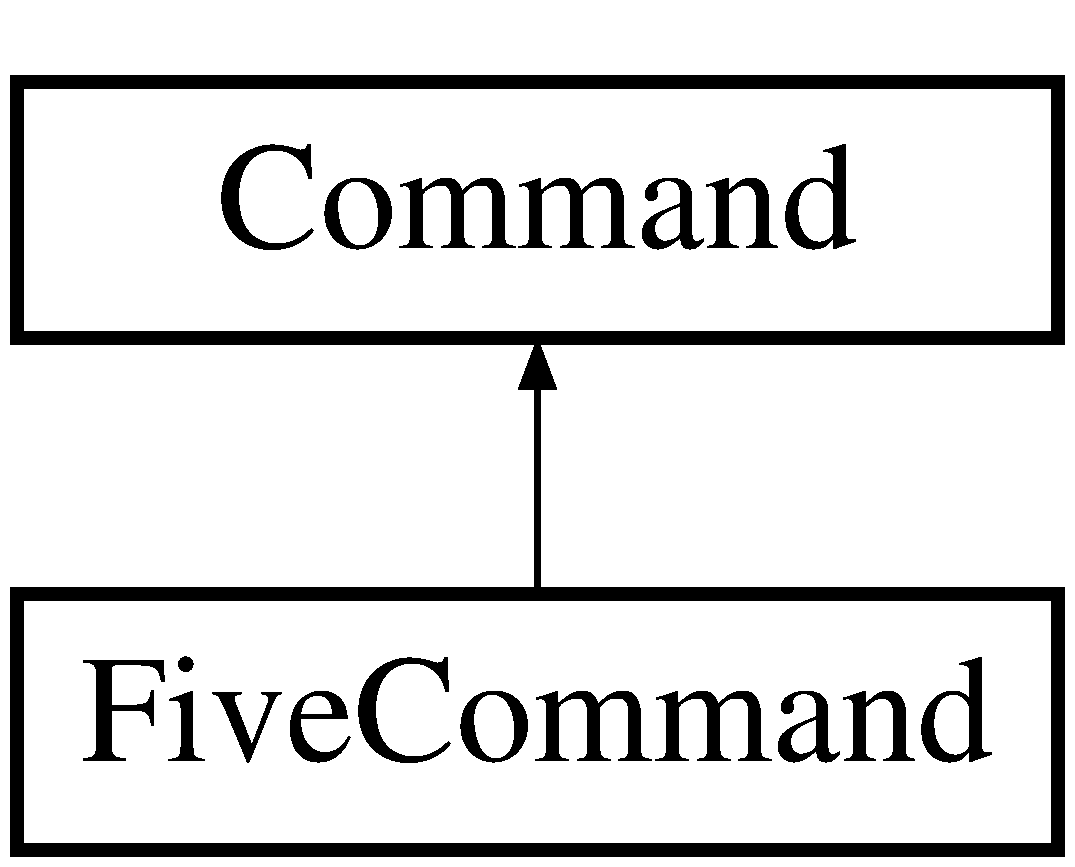
\includegraphics[height=2.000000cm]{class_five_command}
\end{center}
\end{figure}
\subsection*{Public Member Functions}
\begin{DoxyCompactItemize}
\item 
\hypertarget{class_five_command_a7c39ae9c28cfcc1419acc180215ba3ba}{}{\bfseries Five\+Command} (\hyperlink{class_calculator}{Calculator} $\ast$new\+Calc)\label{class_five_command_a7c39ae9c28cfcc1419acc180215ba3ba}

\item 
\hypertarget{class_five_command_a97cbe6f79a00cf03fc8af1dc527dc801}{}void {\bfseries execute} ()\label{class_five_command_a97cbe6f79a00cf03fc8af1dc527dc801}

\end{DoxyCompactItemize}
\subsection*{Public Attributes}
\begin{DoxyCompactItemize}
\item 
\hypertarget{class_five_command_a9c6694f2dff27fabf44a4bacdbb07d12}{}\hyperlink{class_calculator}{Calculator} $\ast$ {\bfseries calculator}\label{class_five_command_a9c6694f2dff27fabf44a4bacdbb07d12}

\end{DoxyCompactItemize}


The documentation for this class was generated from the following files\+:\begin{DoxyCompactItemize}
\item 
Five\+Command.\+h\item 
Five\+Command.\+cpp\end{DoxyCompactItemize}

\hypertarget{class_four_command}{}\section{Four\+Command Class Reference}
\label{class_four_command}\index{Four\+Command@{Four\+Command}}
Inheritance diagram for Four\+Command\+:\begin{figure}[H]
\begin{center}
\leavevmode
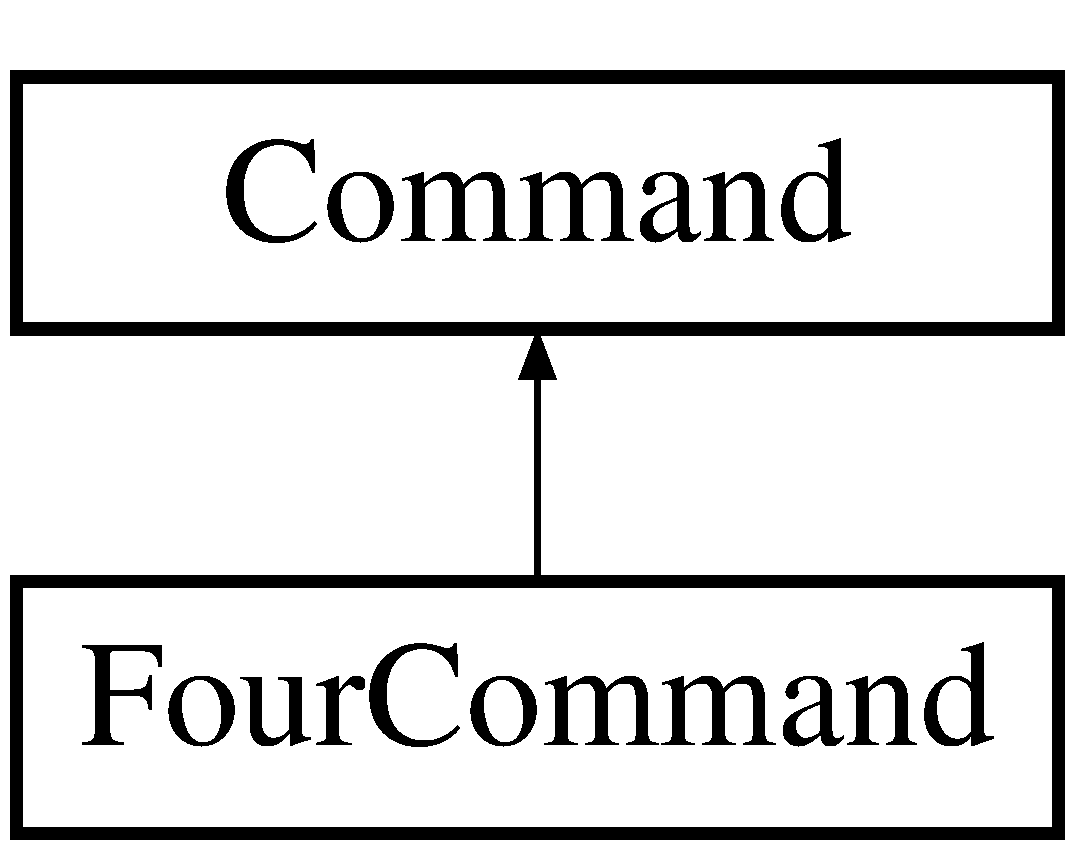
\includegraphics[height=2.000000cm]{class_four_command}
\end{center}
\end{figure}
\subsection*{Public Member Functions}
\begin{DoxyCompactItemize}
\item 
\hypertarget{class_four_command_acba8d0c8c5e4951816c271015f22095e}{}{\bfseries Four\+Command} (\hyperlink{class_calculator}{Calculator} $\ast$new\+Calc)\label{class_four_command_acba8d0c8c5e4951816c271015f22095e}

\item 
\hypertarget{class_four_command_abc26a6d79d1897ab73b963f7737315ef}{}void {\bfseries execute} ()\label{class_four_command_abc26a6d79d1897ab73b963f7737315ef}

\end{DoxyCompactItemize}
\subsection*{Public Attributes}
\begin{DoxyCompactItemize}
\item 
\hypertarget{class_four_command_a3a411398976791c35d4a3c131f592116}{}\hyperlink{class_calculator}{Calculator} $\ast$ {\bfseries calculator}\label{class_four_command_a3a411398976791c35d4a3c131f592116}

\end{DoxyCompactItemize}


The documentation for this class was generated from the following files\+:\begin{DoxyCompactItemize}
\item 
Four\+Command.\+h\item 
Four\+Command.\+cpp\end{DoxyCompactItemize}

\hypertarget{class_input_screen_state}{}\section{Input\+Screen\+State Class Reference}
\label{class_input_screen_state}\index{Input\+Screen\+State@{Input\+Screen\+State}}
Inheritance diagram for Input\+Screen\+State\+:\begin{figure}[H]
\begin{center}
\leavevmode
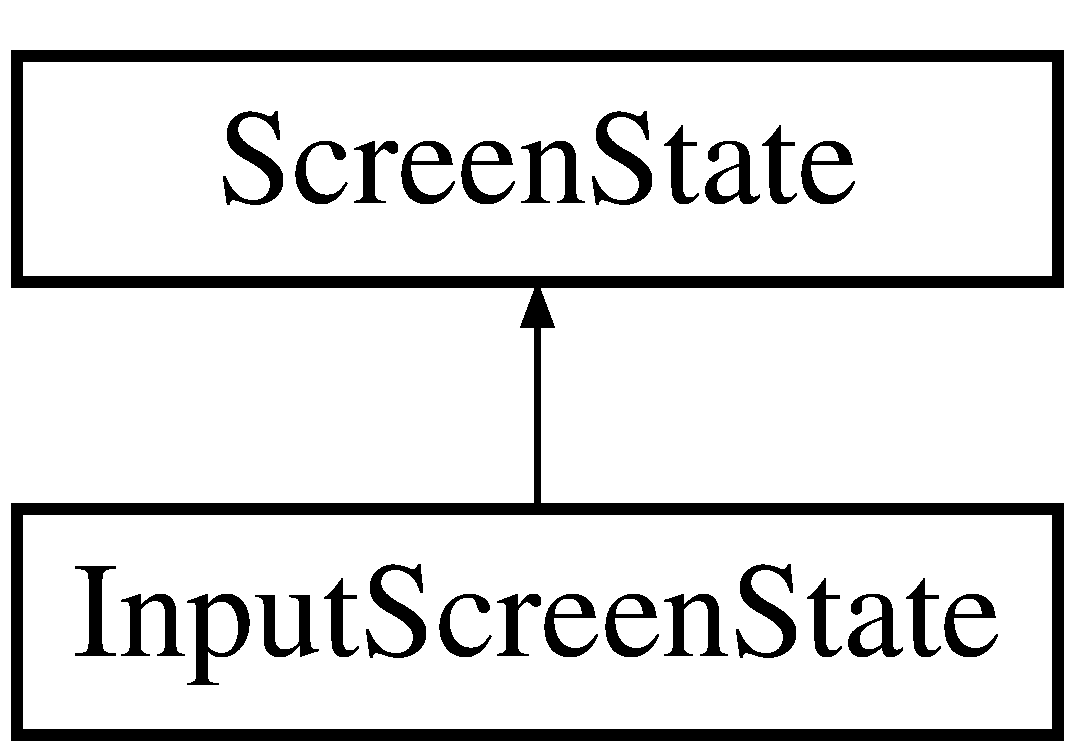
\includegraphics[height=2.000000cm]{class_input_screen_state}
\end{center}
\end{figure}
\subsection*{Public Member Functions}
\begin{DoxyCompactItemize}
\item 
void \hyperlink{class_input_screen_state_acc41e5841cd19d4a55603793b6fb8180}{set\+Screen} (\hyperlink{class_screen}{Screen} $\ast$new\+Screen)
\begin{DoxyCompactList}\small\item\em Set new screen. \end{DoxyCompactList}\item 
void \hyperlink{class_input_screen_state_a2189d602f5fe02660488a5a49c4c76f8}{input} (std\+::string new\+Symbol)
\begin{DoxyCompactList}\small\item\em Input new symbol to the screan according current state. \end{DoxyCompactList}\item 
\hypertarget{class_input_screen_state_a1c2b747f0aa827cc5d60c56c154d4573}{}void \hyperlink{class_input_screen_state_a1c2b747f0aa827cc5d60c56c154d4573}{clear} ()\label{class_input_screen_state_a1c2b747f0aa827cc5d60c56c154d4573}

\begin{DoxyCompactList}\small\item\em Clear screen according state. \end{DoxyCompactList}\end{DoxyCompactItemize}
\subsection*{Static Public Member Functions}
\begin{DoxyCompactItemize}
\item 
\hypertarget{class_input_screen_state_acc5cad3f3defa6541ecea1921e2ce32e}{}static \hyperlink{class_input_screen_state}{Input\+Screen\+State} \& {\bfseries Instance} ()\label{class_input_screen_state_acc5cad3f3defa6541ecea1921e2ce32e}

\end{DoxyCompactItemize}
\subsection*{Public Attributes}
\begin{DoxyCompactItemize}
\item 
\hypertarget{class_input_screen_state_acd38c9445389e3995fec2c4f9763637b}{}\hyperlink{class_screen}{Screen} $\ast$ {\bfseries screen}\label{class_input_screen_state_acd38c9445389e3995fec2c4f9763637b}

\end{DoxyCompactItemize}


\subsection{Member Function Documentation}
\hypertarget{class_input_screen_state_a2189d602f5fe02660488a5a49c4c76f8}{}\index{Input\+Screen\+State@{Input\+Screen\+State}!input@{input}}
\index{input@{input}!Input\+Screen\+State@{Input\+Screen\+State}}
\subsubsection[{input(std\+::string new\+Symbol)}]{\setlength{\rightskip}{0pt plus 5cm}void Input\+Screen\+State\+::input (
\begin{DoxyParamCaption}
\item[{std\+::string}]{new\+Symbol}
\end{DoxyParamCaption}
)\hspace{0.3cm}{\ttfamily [virtual]}}\label{class_input_screen_state_a2189d602f5fe02660488a5a49c4c76f8}


Input new symbol to the screan according current state. 


\begin{DoxyParams}{Parameters}
{\em new\+Symbol} & \\
\hline
\end{DoxyParams}


Implements \hyperlink{class_screen_state_adb71081141ec6c066d54f1dc77c78717}{Screen\+State}.

\hypertarget{class_input_screen_state_acc41e5841cd19d4a55603793b6fb8180}{}\index{Input\+Screen\+State@{Input\+Screen\+State}!set\+Screen@{set\+Screen}}
\index{set\+Screen@{set\+Screen}!Input\+Screen\+State@{Input\+Screen\+State}}
\subsubsection[{set\+Screen(\+Screen $\ast$new\+Screen)}]{\setlength{\rightskip}{0pt plus 5cm}void Input\+Screen\+State\+::set\+Screen (
\begin{DoxyParamCaption}
\item[{{\bf Screen} $\ast$}]{new\+Screen}
\end{DoxyParamCaption}
)}\label{class_input_screen_state_acc41e5841cd19d4a55603793b6fb8180}


Set new screen. 


\begin{DoxyParams}{Parameters}
{\em new\+Screen} & \mbox{[}description\mbox{]} \\
\hline
\end{DoxyParams}


The documentation for this class was generated from the following files\+:\begin{DoxyCompactItemize}
\item 
Input\+Screen\+State.\+h\item 
Input\+Screen\+State.\+cpp\end{DoxyCompactItemize}

\hypertarget{class_invoker}{}\section{Invoker Class Reference}
\label{class_invoker}\index{Invoker@{Invoker}}


{\ttfamily \#include $<$Invoker.\+h$>$}

\subsection*{Public Member Functions}
\begin{DoxyCompactItemize}
\item 
\hyperlink{class_invoker_a23a9f865dabc7f79cf27085d6aabbc81}{Invoker} ()
\item 
\hypertarget{class_invoker_a85b4ed1f7a614fd301a927eea9aebd34}{}void {\bfseries set\+Command} (\hyperlink{class_command}{Command} $\ast$new\+Command)\label{class_invoker_a85b4ed1f7a614fd301a927eea9aebd34}

\item 
\hypertarget{class_invoker_abb638c8a0375ffe8b8bc36807bc34feb}{}void {\bfseries run} ()\label{class_invoker_abb638c8a0375ffe8b8bc36807bc34feb}

\end{DoxyCompactItemize}
\subsection*{Public Attributes}
\begin{DoxyCompactItemize}
\item 
\hypertarget{class_invoker_a66787cc9fe2056889d2d091bb9759892}{}\hyperlink{class_command}{Command} $\ast$ {\bfseries command}\label{class_invoker_a66787cc9fe2056889d2d091bb9759892}

\end{DoxyCompactItemize}


\subsection{Detailed Description}
Calculator -\/ Simple calculator realization by patterns Copyright (C) 2017 -\/ ? Alexey Konyshev (\href{mailto:aleksey.konyshev@gmail.com}{\tt aleksey.\+konyshev@gmail.\+com})

This software is provided \textquotesingle{}as-\/is\textquotesingle{}, without any express or implied warranty. In no event will the authors be held liable for any damages arising from the use of this software.

Permission is granted to anyone to use this software for any purpose, including commercial applications, and to alter it and redistribute it freely, subject to the following restrictions\+:


\begin{DoxyEnumerate}
\item The origin of this software must not be misrepresented; you must not claim that you wrote the original software. If you use this software in a product, an acknowledgment in the product documentation would be appreciated but is not required.
\item Altered source versions must be plainly marked as such, and must not be misrepresented as being the original software.
\item This notice may not be removed or altered from any source distribution. 
\end{DoxyEnumerate}

\subsection{Constructor \& Destructor Documentation}
\hypertarget{class_invoker_a23a9f865dabc7f79cf27085d6aabbc81}{}\index{Invoker@{Invoker}!Invoker@{Invoker}}
\index{Invoker@{Invoker}!Invoker@{Invoker}}
\subsubsection[{Invoker()}]{\setlength{\rightskip}{0pt plus 5cm}Invoker\+::\+Invoker (
\begin{DoxyParamCaption}
{}
\end{DoxyParamCaption}
)}\label{class_invoker_a23a9f865dabc7f79cf27085d6aabbc81}
Calculator -\/ Simple calculator realization by patterns Copyright (C) 2017 -\/ ? Alexey Konyshev (\href{mailto:aleksey.konyshev@gmail.com}{\tt aleksey.\+konyshev@gmail.\+com})

This software is provided \textquotesingle{}as-\/is\textquotesingle{}, without any express or implied warranty. In no event will the authors be held liable for any damages arising from the use of this software.

Permission is granted to anyone to use this software for any purpose, including commercial applications, and to alter it and redistribute it freely, subject to the following restrictions\+:


\begin{DoxyEnumerate}
\item The origin of this software must not be misrepresented; you must not claim that you wrote the original software. If you use this software in a product, an acknowledgment in the product documentation would be appreciated but is not required.
\item Altered source versions must be plainly marked as such, and must not be misrepresented as being the original software.
\item This notice may not be removed or altered from any source distribution. 
\end{DoxyEnumerate}

The documentation for this class was generated from the following files\+:\begin{DoxyCompactItemize}
\item 
Invoker.\+h\item 
Invoker.\+cpp\end{DoxyCompactItemize}

\hypertarget{class_math_op}{}\section{Math\+Op Class Reference}
\label{class_math_op}\index{Math\+Op@{Math\+Op}}
Inheritance diagram for Math\+Op\+:\begin{figure}[H]
\begin{center}
\leavevmode
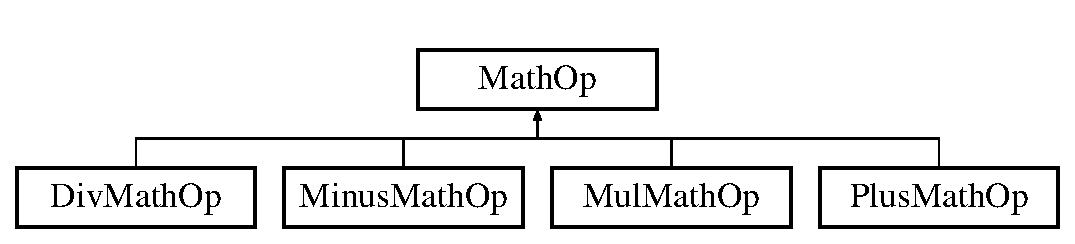
\includegraphics[height=2.000000cm]{class_math_op}
\end{center}
\end{figure}
\subsection*{Public Member Functions}
\begin{DoxyCompactItemize}
\item 
\hypertarget{class_math_op_a7eb54cf02054e4c65afd93f0e1f54833}{}virtual void {\bfseries execute} ()=0\label{class_math_op_a7eb54cf02054e4c65afd93f0e1f54833}

\item 
\hypertarget{class_math_op_aaf00128f671302d984bb32e488229616}{}void {\bfseries set\+A} (double new\+A)\label{class_math_op_aaf00128f671302d984bb32e488229616}

\item 
\hypertarget{class_math_op_a99e27af1ed722c942d4018b7384b0dff}{}void {\bfseries set\+A\+B} (double new\+A, double new\+B)\label{class_math_op_a99e27af1ed722c942d4018b7384b0dff}

\item 
\hypertarget{class_math_op_a45e51beba01736ca71ccd641eec4b433}{}double {\bfseries get\+Result} ()\label{class_math_op_a45e51beba01736ca71ccd641eec4b433}

\end{DoxyCompactItemize}
\subsection*{Public Attributes}
\begin{DoxyCompactItemize}
\item 
\hypertarget{class_math_op_afa40241343dc3c5d550e13c45ec3a958}{}double {\bfseries a}\label{class_math_op_afa40241343dc3c5d550e13c45ec3a958}

\item 
\hypertarget{class_math_op_afff7e10b49bb685057eea3b6cd1cdd90}{}double {\bfseries b}\label{class_math_op_afff7e10b49bb685057eea3b6cd1cdd90}

\item 
\hypertarget{class_math_op_a156f7ed952cbc7b0efe5a53cb3706d88}{}double {\bfseries result}\label{class_math_op_a156f7ed952cbc7b0efe5a53cb3706d88}

\item 
\hypertarget{class_math_op_ae747c21140de4a79fada80575519ca22}{}std\+::string {\bfseries math\+Op\+Name}\label{class_math_op_ae747c21140de4a79fada80575519ca22}

\end{DoxyCompactItemize}


The documentation for this class was generated from the following files\+:\begin{DoxyCompactItemize}
\item 
Math\+Op.\+h\item 
Math\+Op.\+cpp\end{DoxyCompactItemize}

\hypertarget{class_math_op_list}{}\section{Math\+Op\+List Class Reference}
\label{class_math_op_list}\index{Math\+Op\+List@{Math\+Op\+List}}
\subsection*{Public Member Functions}
\begin{DoxyCompactItemize}
\item 
\hypertarget{class_math_op_list_a5316d3bc11507fbb0c1accc8f50ef44b}{}void {\bfseries add\+Operation} (\hyperlink{class_math_op}{Math\+Op} $\ast$new\+Math\+Op)\label{class_math_op_list_a5316d3bc11507fbb0c1accc8f50ef44b}

\item 
\hypertarget{class_math_op_list_a8a8912d6b56b82ce57c2f8438ffcf1c3}{}void {\bfseries remove\+Operation} (int pos)\label{class_math_op_list_a8a8912d6b56b82ce57c2f8438ffcf1c3}

\item 
\hypertarget{class_math_op_list_a03cb8ae4c430d44ad0da52f92e08dce9}{}bool {\bfseries has\+Next} ()\label{class_math_op_list_a03cb8ae4c430d44ad0da52f92e08dce9}

\item 
\hypertarget{class_math_op_list_aea70a75d82a00034f5f2fb2aa5b16b22}{}void {\bfseries set\+Head\+Pos} ()\label{class_math_op_list_aea70a75d82a00034f5f2fb2aa5b16b22}

\item 
\hypertarget{class_math_op_list_a20880de2f17a1f883b5254603325e38f}{}\hyperlink{class_math_op}{Math\+Op} $\ast$ {\bfseries get\+Last} ()\label{class_math_op_list_a20880de2f17a1f883b5254603325e38f}

\item 
\hypertarget{class_math_op_list_ad062e78175b80791fa07ee08f4dbe0d5}{}int {\bfseries get\+Last\+Pos} ()\label{class_math_op_list_ad062e78175b80791fa07ee08f4dbe0d5}

\item 
\hypertarget{class_math_op_list_a57a567366dd8f83779d6040c9fb017c4}{}\hyperlink{class_math_op}{Math\+Op} $\ast$ {\bfseries get} ()\label{class_math_op_list_a57a567366dd8f83779d6040c9fb017c4}

\item 
\hypertarget{class_math_op_list_a4c6555e072ee3280f8d7fd93551f4513}{}\hyperlink{class_math_op}{Math\+Op} $\ast$ {\bfseries get} (int pos)\label{class_math_op_list_a4c6555e072ee3280f8d7fd93551f4513}

\item 
\hypertarget{class_math_op_list_a18e3ee1871a887d1428072f98f1c5cbd}{}bool {\bfseries is\+Empty} ()\label{class_math_op_list_a18e3ee1871a887d1428072f98f1c5cbd}

\end{DoxyCompactItemize}
\subsection*{Public Attributes}
\begin{DoxyCompactItemize}
\item 
\hypertarget{class_math_op_list_a4ac4dea48bead1d889e92b41c3d99c49}{}\hyperlink{class_math_op}{Math\+Op} $\ast$$\ast$ {\bfseries math\+Ops\+List}\label{class_math_op_list_a4ac4dea48bead1d889e92b41c3d99c49}

\item 
\hypertarget{class_math_op_list_afe8625a3d84f8654d9f0a7a91fd6f72f}{}int {\bfseries size}\label{class_math_op_list_afe8625a3d84f8654d9f0a7a91fd6f72f}

\item 
\hypertarget{class_math_op_list_a3ea410994e07a06ce9d177c639b514a2}{}int {\bfseries current\+Pos}\label{class_math_op_list_a3ea410994e07a06ce9d177c639b514a2}

\item 
\hypertarget{class_math_op_list_a7ee46ef2288f804bc6f6241e42e97093}{}int {\bfseries last\+Operation}\label{class_math_op_list_a7ee46ef2288f804bc6f6241e42e97093}

\end{DoxyCompactItemize}


The documentation for this class was generated from the following files\+:\begin{DoxyCompactItemize}
\item 
Math\+Op\+List.\+h\item 
Math\+Op\+List.\+cpp\end{DoxyCompactItemize}

\hypertarget{class_minus_command}{}\section{Minus\+Command Class Reference}
\label{class_minus_command}\index{Minus\+Command@{Minus\+Command}}
Inheritance diagram for Minus\+Command\+:\begin{figure}[H]
\begin{center}
\leavevmode
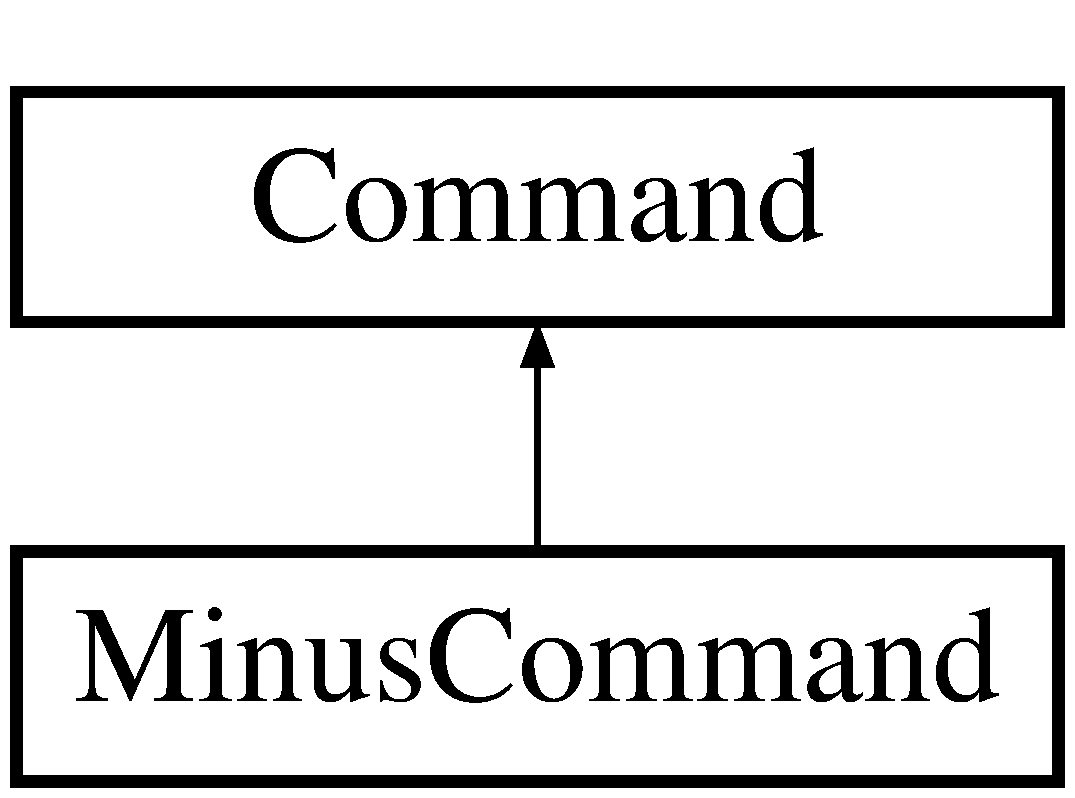
\includegraphics[height=2.000000cm]{class_minus_command}
\end{center}
\end{figure}
\subsection*{Public Member Functions}
\begin{DoxyCompactItemize}
\item 
\hypertarget{class_minus_command_a9304469f5f5baa79902bd21e81fb3526}{}{\bfseries Minus\+Command} (\hyperlink{class_calculator}{Calculator} $\ast$new\+Calc)\label{class_minus_command_a9304469f5f5baa79902bd21e81fb3526}

\item 
\hypertarget{class_minus_command_a117f4a7fb5f380d968e057ee9efad956}{}void {\bfseries execute} ()\label{class_minus_command_a117f4a7fb5f380d968e057ee9efad956}

\end{DoxyCompactItemize}
\subsection*{Public Attributes}
\begin{DoxyCompactItemize}
\item 
\hypertarget{class_minus_command_a659a458964a22955e73022f23c8a2f7e}{}\hyperlink{class_calculator}{Calculator} $\ast$ {\bfseries calculator}\label{class_minus_command_a659a458964a22955e73022f23c8a2f7e}

\end{DoxyCompactItemize}


The documentation for this class was generated from the following files\+:\begin{DoxyCompactItemize}
\item 
Minus\+Command.\+h\item 
Minus\+Command.\+cpp\end{DoxyCompactItemize}

\hypertarget{class_minus_math_op}{}\section{Minus\+Math\+Op Class Reference}
\label{class_minus_math_op}\index{Minus\+Math\+Op@{Minus\+Math\+Op}}
Inheritance diagram for Minus\+Math\+Op\+:\begin{figure}[H]
\begin{center}
\leavevmode
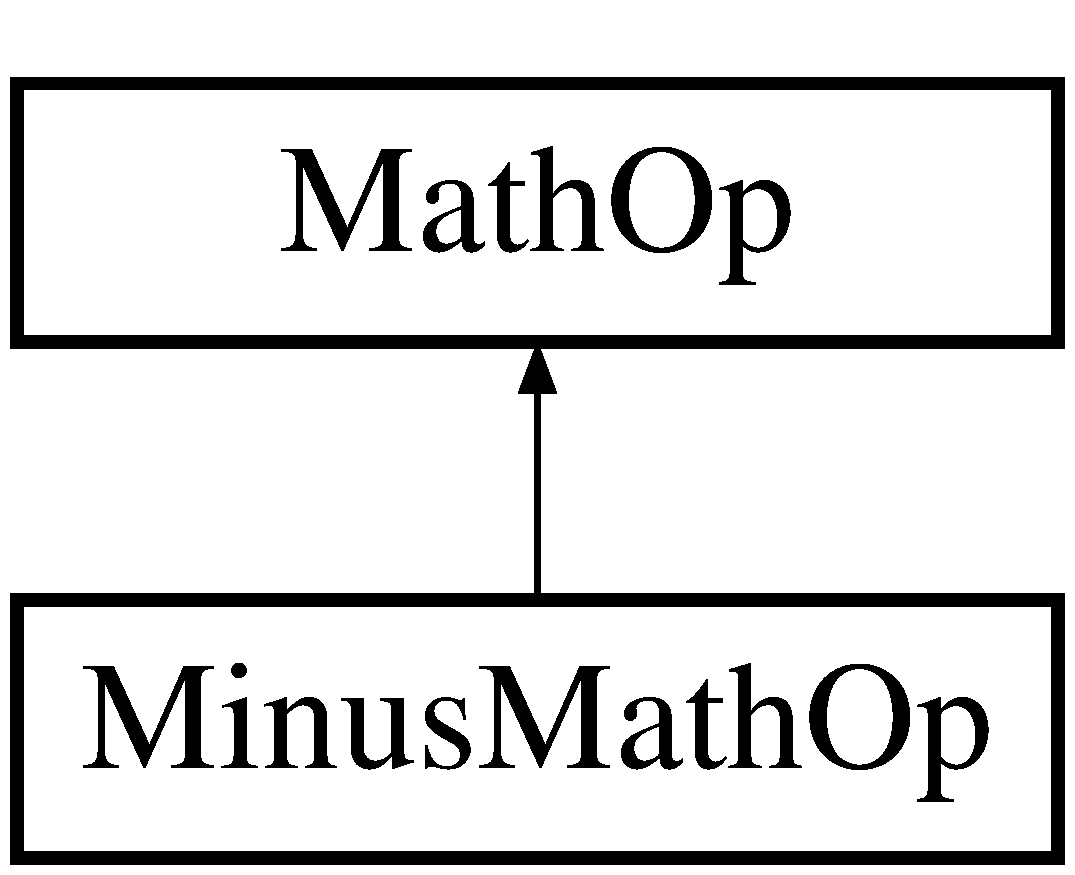
\includegraphics[height=2.000000cm]{class_minus_math_op}
\end{center}
\end{figure}
\subsection*{Public Member Functions}
\begin{DoxyCompactItemize}
\item 
\hypertarget{class_minus_math_op_a996c6bc342830c935e02c0752feb3500}{}void {\bfseries execute} ()\label{class_minus_math_op_a996c6bc342830c935e02c0752feb3500}

\end{DoxyCompactItemize}
\subsection*{Additional Inherited Members}


The documentation for this class was generated from the following files\+:\begin{DoxyCompactItemize}
\item 
Minus\+Math\+Op.\+h\item 
Minus\+Math\+Op.\+cpp\end{DoxyCompactItemize}

\hypertarget{class_mul_command}{}\section{Mul\+Command Class Reference}
\label{class_mul_command}\index{Mul\+Command@{Mul\+Command}}


implementations of multiply command  




{\ttfamily \#include $<$Mul\+Command.\+h$>$}

Inheritance diagram for Mul\+Command\+:\begin{figure}[H]
\begin{center}
\leavevmode
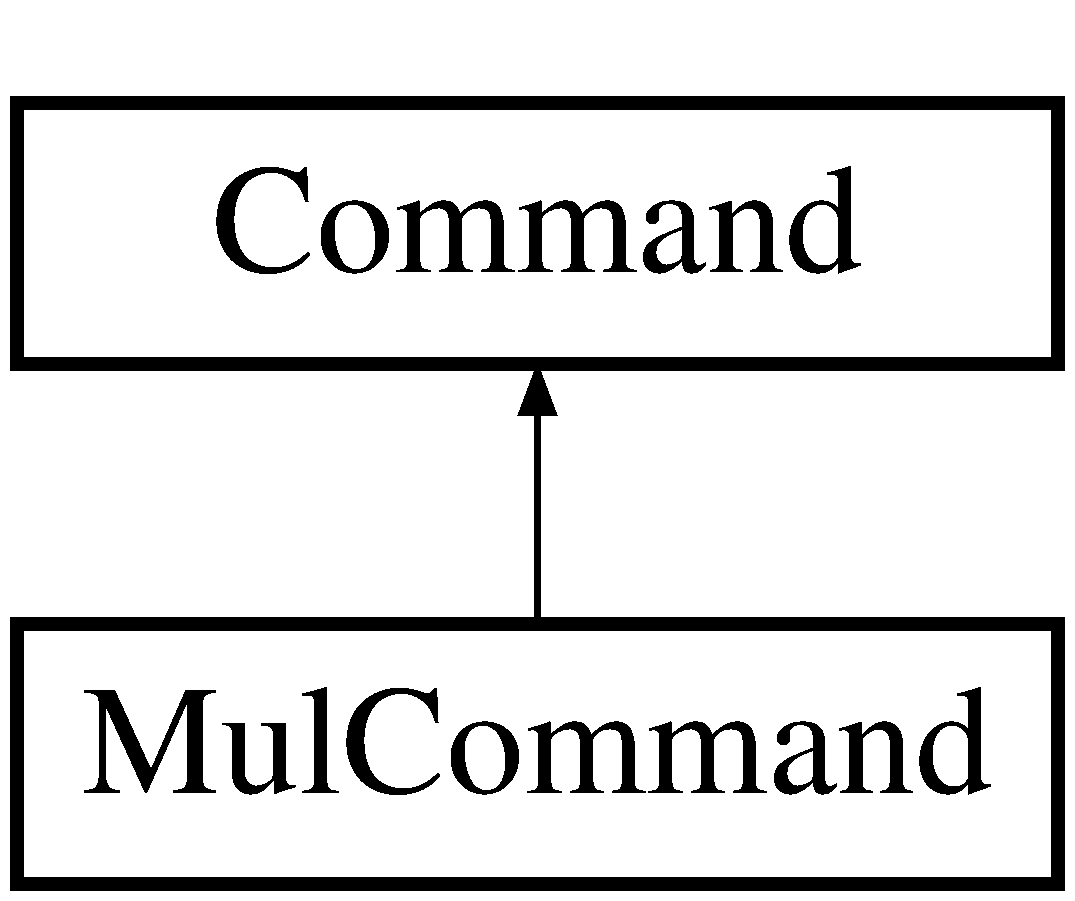
\includegraphics[height=2.000000cm]{class_mul_command}
\end{center}
\end{figure}
\subsection*{Public Member Functions}
\begin{DoxyCompactItemize}
\item 
\hyperlink{class_mul_command_ad841942b274629dd6ef16ebff60adc0d}{Mul\+Command} (Calculator $\ast$new\+Calc)
\begin{DoxyCompactList}\small\item\em A constructor. Sets pointer to the implementation of. \end{DoxyCompactList}\item 
\hyperlink{class_mul_command_ac298a4978766f69cd13e8258793a6de1}{$\sim$\+Mul\+Command} ()
\item 
void \hyperlink{class_mul_command_a26122a47a8ddbca2b7a6a3991e04ed66}{execute} ()
\begin{DoxyCompactList}\small\item\em Executes mul command of. \end{DoxyCompactList}\end{DoxyCompactItemize}
\subsection*{Public Attributes}
\begin{DoxyCompactItemize}
\item 
Calculator $\ast$ \hyperlink{class_mul_command_ad1f527968e768963a14e1b59825022d0}{calculator}
\end{DoxyCompactItemize}


\subsection{Detailed Description}
implementations of multiply command 

Calculator -\/ Simple calculator realization by patterns Copyright (C) 2017 -\/ ? Alexey Konyshev (\href{mailto:aleksey.konyshev@gmail.com}{\tt aleksey.\+konyshev@gmail.\+com})

This software is provided \textquotesingle{}as-\/is\textquotesingle{}, without any express or implied warranty. In no event will the authors be held liable for any damages arising from the use of this software.

Permission is granted to anyone to use this software for any purpose, including commercial applications, and to alter it and redistribute it freely, subject to the following restrictions\+:


\begin{DoxyEnumerate}
\item The origin of this software must not be misrepresented; you must not claim that you wrote the original software. If you use this software in a product, an acknowledgment in the product documentation would be appreciated but is not required.
\item Altered source versions must be plainly marked as such, and must not be misrepresented as being the original software.
\item This notice may not be removed or altered from any source distribution. Headers 
\begin{DoxyCode}
\hyperlink{class_command}{Command} 
\end{DoxyCode}
 
\end{DoxyEnumerate}

\subsection{Constructor \& Destructor Documentation}
\hypertarget{class_mul_command_ad841942b274629dd6ef16ebff60adc0d}{}\index{Mul\+Command@{Mul\+Command}!Mul\+Command@{Mul\+Command}}
\index{Mul\+Command@{Mul\+Command}!Mul\+Command@{Mul\+Command}}
\subsubsection[{Mul\+Command(\+Calculator $\ast$new\+Calc)}]{\setlength{\rightskip}{0pt plus 5cm}Mul\+Command\+::\+Mul\+Command (
\begin{DoxyParamCaption}
\item[{Calculator $\ast$}]{new\+Calc}
\end{DoxyParamCaption}
)}\label{class_mul_command_ad841942b274629dd6ef16ebff60adc0d}


A constructor. Sets pointer to the implementation of. 


\begin{DoxyCode}
Calculator 
\end{DoxyCode}



\begin{DoxyParams}{Parameters}
{\em new\+Calc} & a new
\begin{DoxyCode}
Calculator 
\end{DoxyCode}
\\
\hline
\end{DoxyParams}
Calculator -\/ Simple calculator realization by patterns Copyright (C) 2017 -\/ ? Alexey Konyshev (\href{mailto:aleksey.konyshev@gmail.com}{\tt aleksey.\+konyshev@gmail.\+com})

This software is provided \textquotesingle{}as-\/is\textquotesingle{}, without any express or implied warranty. In no event will the authors be held liable for any damages arising from the use of this software.

Permission is granted to anyone to use this software for any purpose, including commercial applications, and to alter it and redistribute it freely, subject to the following restrictions\+:


\begin{DoxyEnumerate}
\item The origin of this software must not be misrepresented; you must not claim that you wrote the original software. If you use this software in a product, an acknowledgment in the product documentation would be appreciated but is not required.
\item Altered source versions must be plainly marked as such, and must not be misrepresented as being the original software.
\item This notice may not be removed or altered from any source distribution. Headers 
\end{DoxyEnumerate}\hypertarget{class_mul_command_ac298a4978766f69cd13e8258793a6de1}{}\index{Mul\+Command@{Mul\+Command}!````~Mul\+Command@{$\sim$\+Mul\+Command}}
\index{````~Mul\+Command@{$\sim$\+Mul\+Command}!Mul\+Command@{Mul\+Command}}
\subsubsection[{$\sim$\+Mul\+Command()}]{\setlength{\rightskip}{0pt plus 5cm}Mul\+Command\+::$\sim$\+Mul\+Command (
\begin{DoxyParamCaption}
{}
\end{DoxyParamCaption}
)}\label{class_mul_command_ac298a4978766f69cd13e8258793a6de1}
A destructor 

\subsection{Member Function Documentation}
\hypertarget{class_mul_command_a26122a47a8ddbca2b7a6a3991e04ed66}{}\index{Mul\+Command@{Mul\+Command}!execute@{execute}}
\index{execute@{execute}!Mul\+Command@{Mul\+Command}}
\subsubsection[{execute()}]{\setlength{\rightskip}{0pt plus 5cm}void Mul\+Command\+::execute (
\begin{DoxyParamCaption}
{}
\end{DoxyParamCaption}
)\hspace{0.3cm}{\ttfamily [virtual]}}\label{class_mul_command_a26122a47a8ddbca2b7a6a3991e04ed66}


Executes mul command of. 


\begin{DoxyCode}
Calculator 
\end{DoxyCode}
 \begin{DoxySeeAlso}{See also}

\begin{DoxyCode}
Calculator::Mul() 
\end{DoxyCode}
 
\end{DoxySeeAlso}


Implements \hyperlink{class_command_a6fd7d9bd8df8bfc881e4d6c7cd1878b7}{Command}.



\subsection{Member Data Documentation}
\hypertarget{class_mul_command_ad1f527968e768963a14e1b59825022d0}{}\index{Mul\+Command@{Mul\+Command}!calculator@{calculator}}
\index{calculator@{calculator}!Mul\+Command@{Mul\+Command}}
\subsubsection[{calculator}]{\setlength{\rightskip}{0pt plus 5cm}Calculator$\ast$ Mul\+Command\+::calculator}\label{class_mul_command_ad1f527968e768963a14e1b59825022d0}
pointer to the
\begin{DoxyCode}
Calculator 
\end{DoxyCode}
 

The documentation for this class was generated from the following files\+:\begin{DoxyCompactItemize}
\item 
Mul\+Command.\+h\item 
Mul\+Command.\+cpp\end{DoxyCompactItemize}

\hypertarget{class_mul_math_op}{}\section{Mul\+Math\+Op Class Reference}
\label{class_mul_math_op}\index{Mul\+Math\+Op@{Mul\+Math\+Op}}
Inheritance diagram for Mul\+Math\+Op\+:\begin{figure}[H]
\begin{center}
\leavevmode
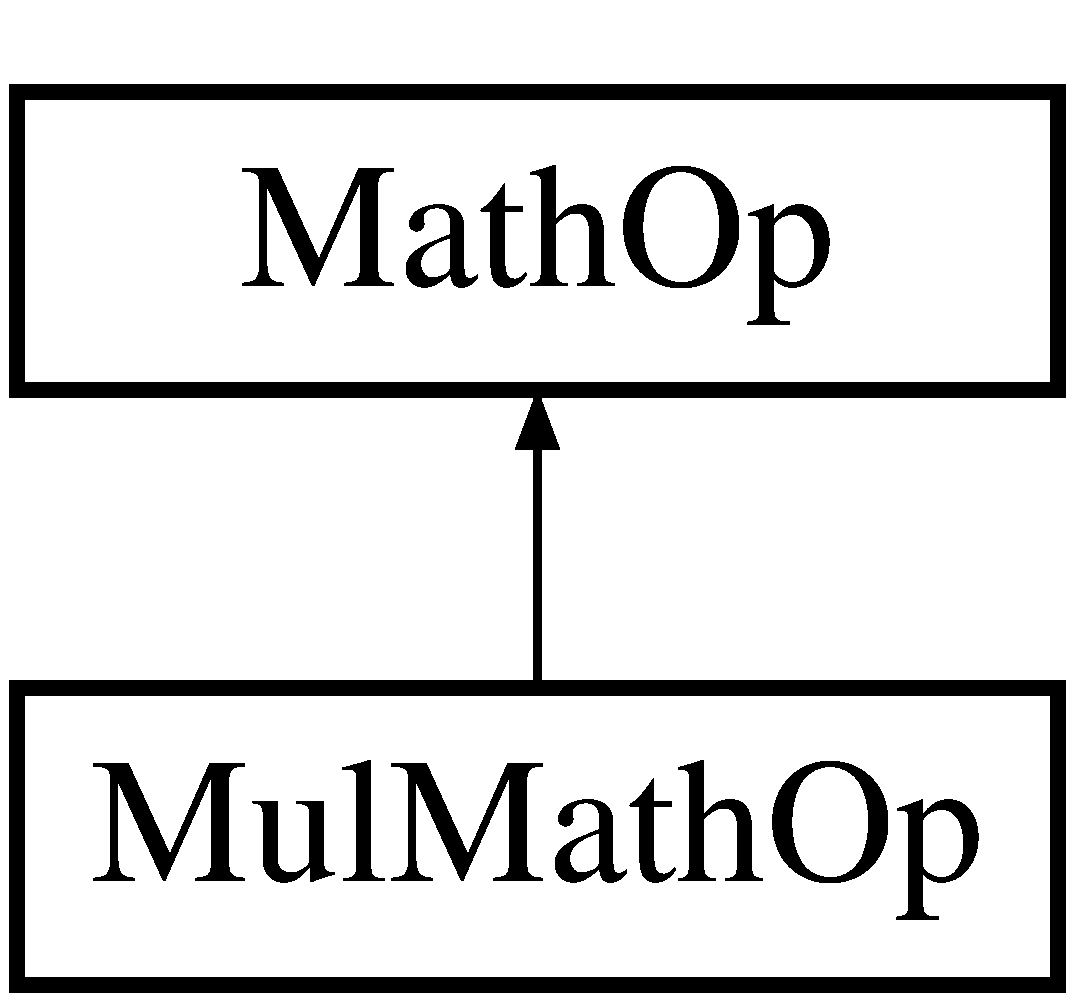
\includegraphics[height=2.000000cm]{class_mul_math_op}
\end{center}
\end{figure}
\subsection*{Public Member Functions}
\begin{DoxyCompactItemize}
\item 
\hypertarget{class_mul_math_op_a21cfc2fe66be9eb5dc5a96d80a06bc05}{}void {\bfseries execute} ()\label{class_mul_math_op_a21cfc2fe66be9eb5dc5a96d80a06bc05}

\end{DoxyCompactItemize}
\subsection*{Additional Inherited Members}


The documentation for this class was generated from the following files\+:\begin{DoxyCompactItemize}
\item 
Mul\+Math\+Op.\+h\item 
Mul\+Math\+Op.\+cpp\end{DoxyCompactItemize}

\hypertarget{class_nine_command}{}\section{Nine\+Command Class Reference}
\label{class_nine_command}\index{Nine\+Command@{Nine\+Command}}


implementations of nine command  




{\ttfamily \#include $<$Nine\+Command.\+h$>$}

Inheritance diagram for Nine\+Command\+:\begin{figure}[H]
\begin{center}
\leavevmode
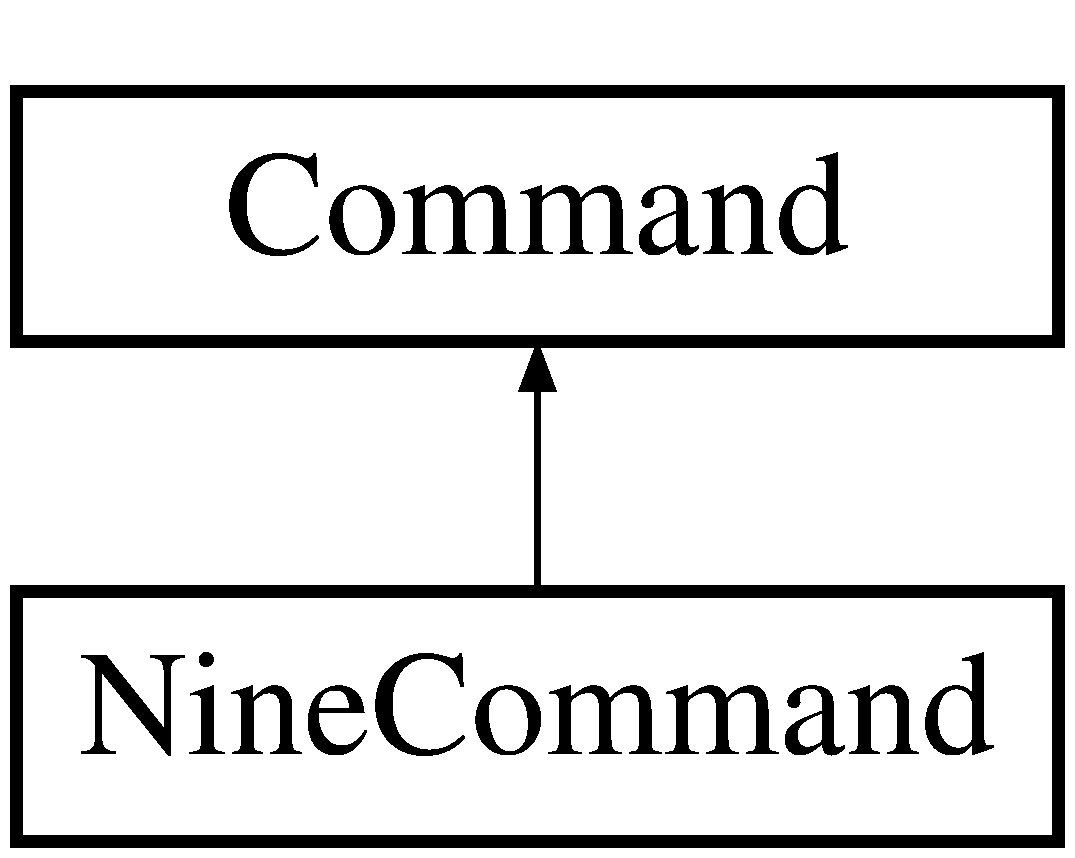
\includegraphics[height=2.000000cm]{class_nine_command}
\end{center}
\end{figure}
\subsection*{Public Member Functions}
\begin{DoxyCompactItemize}
\item 
\hyperlink{class_nine_command_a44f89f6ad7fa2a153d4900ae3553bd68}{Nine\+Command} (Calculator $\ast$new\+Calc)
\begin{DoxyCompactList}\small\item\em A constructor. Sets pointer to the implementation of. \end{DoxyCompactList}\item 
\hyperlink{class_nine_command_a0c5450cc5e1663bdacb821de8c5c94e7}{$\sim$\+Nine\+Command} ()
\item 
void \hyperlink{class_nine_command_a8574ee5eab651afee7426db0fe2cb2f0}{execute} ()
\begin{DoxyCompactList}\small\item\em Executes nine command of. \end{DoxyCompactList}\end{DoxyCompactItemize}
\subsection*{Public Attributes}
\begin{DoxyCompactItemize}
\item 
Calculator $\ast$ \hyperlink{class_nine_command_a3bb8db5764e5c2e3e2025dadf1f81a96}{calculator}
\end{DoxyCompactItemize}


\subsection{Detailed Description}
implementations of nine command 

Calculator -\/ Simple calculator realization by patterns Copyright (C) 2017 -\/ ? Alexey Konyshev (\href{mailto:aleksey.konyshev@gmail.com}{\tt aleksey.\+konyshev@gmail.\+com})

This software is provided \textquotesingle{}as-\/is\textquotesingle{}, without any express or implied warranty. In no event will the authors be held liable for any damages arising from the use of this software.

Permission is granted to anyone to use this software for any purpose, including commercial applications, and to alter it and redistribute it freely, subject to the following restrictions\+:


\begin{DoxyEnumerate}
\item The origin of this software must not be misrepresented; you must not claim that you wrote the original software. If you use this software in a product, an acknowledgment in the product documentation would be appreciated but is not required.
\item Altered source versions must be plainly marked as such, and must not be misrepresented as being the original software.
\item This notice may not be removed or altered from any source distribution. Headers 
\begin{DoxyCode}
\hyperlink{class_command}{Command} 
\end{DoxyCode}
 
\end{DoxyEnumerate}

\subsection{Constructor \& Destructor Documentation}
\hypertarget{class_nine_command_a44f89f6ad7fa2a153d4900ae3553bd68}{}\index{Nine\+Command@{Nine\+Command}!Nine\+Command@{Nine\+Command}}
\index{Nine\+Command@{Nine\+Command}!Nine\+Command@{Nine\+Command}}
\subsubsection[{Nine\+Command(\+Calculator $\ast$new\+Calc)}]{\setlength{\rightskip}{0pt plus 5cm}Nine\+Command\+::\+Nine\+Command (
\begin{DoxyParamCaption}
\item[{Calculator $\ast$}]{new\+Calc}
\end{DoxyParamCaption}
)}\label{class_nine_command_a44f89f6ad7fa2a153d4900ae3553bd68}


A constructor. Sets pointer to the implementation of. 


\begin{DoxyCode}
Calculator 
\end{DoxyCode}



\begin{DoxyParams}{Parameters}
{\em new\+Calc} & a new
\begin{DoxyCode}
Calculator 
\end{DoxyCode}
\\
\hline
\end{DoxyParams}
Calculator -\/ Simple calculator realization by patterns Copyright (C) 2017 -\/ ? Alexey Konyshev (\href{mailto:aleksey.konyshev@gmail.com}{\tt aleksey.\+konyshev@gmail.\+com})

This software is provided \textquotesingle{}as-\/is\textquotesingle{}, without any express or implied warranty. In no event will the authors be held liable for any damages arising from the use of this software.

Permission is granted to anyone to use this software for any purpose, including commercial applications, and to alter it and redistribute it freely, subject to the following restrictions\+:


\begin{DoxyEnumerate}
\item The origin of this software must not be misrepresented; you must not claim that you wrote the original software. If you use this software in a product, an acknowledgment in the product documentation would be appreciated but is not required.
\item Altered source versions must be plainly marked as such, and must not be misrepresented as being the original software.
\item This notice may not be removed or altered from any source distribution. Headers 
\end{DoxyEnumerate}\hypertarget{class_nine_command_a0c5450cc5e1663bdacb821de8c5c94e7}{}\index{Nine\+Command@{Nine\+Command}!````~Nine\+Command@{$\sim$\+Nine\+Command}}
\index{````~Nine\+Command@{$\sim$\+Nine\+Command}!Nine\+Command@{Nine\+Command}}
\subsubsection[{$\sim$\+Nine\+Command()}]{\setlength{\rightskip}{0pt plus 5cm}Nine\+Command\+::$\sim$\+Nine\+Command (
\begin{DoxyParamCaption}
{}
\end{DoxyParamCaption}
)}\label{class_nine_command_a0c5450cc5e1663bdacb821de8c5c94e7}
A destructor 

\subsection{Member Function Documentation}
\hypertarget{class_nine_command_a8574ee5eab651afee7426db0fe2cb2f0}{}\index{Nine\+Command@{Nine\+Command}!execute@{execute}}
\index{execute@{execute}!Nine\+Command@{Nine\+Command}}
\subsubsection[{execute()}]{\setlength{\rightskip}{0pt plus 5cm}void Nine\+Command\+::execute (
\begin{DoxyParamCaption}
{}
\end{DoxyParamCaption}
)\hspace{0.3cm}{\ttfamily [virtual]}}\label{class_nine_command_a8574ee5eab651afee7426db0fe2cb2f0}


Executes nine command of. 


\begin{DoxyCode}
Calculator 
\end{DoxyCode}
 \begin{DoxySeeAlso}{See also}

\begin{DoxyCode}
Calculator::Nine() 
\end{DoxyCode}
 
\end{DoxySeeAlso}


Implements \hyperlink{class_command_a6fd7d9bd8df8bfc881e4d6c7cd1878b7}{Command}.



\subsection{Member Data Documentation}
\hypertarget{class_nine_command_a3bb8db5764e5c2e3e2025dadf1f81a96}{}\index{Nine\+Command@{Nine\+Command}!calculator@{calculator}}
\index{calculator@{calculator}!Nine\+Command@{Nine\+Command}}
\subsubsection[{calculator}]{\setlength{\rightskip}{0pt plus 5cm}Calculator$\ast$ Nine\+Command\+::calculator}\label{class_nine_command_a3bb8db5764e5c2e3e2025dadf1f81a96}
pointer to the
\begin{DoxyCode}
Calculator 
\end{DoxyCode}
 

The documentation for this class was generated from the following files\+:\begin{DoxyCompactItemize}
\item 
Nine\+Command.\+h\item 
Nine\+Command.\+cpp\end{DoxyCompactItemize}

\hypertarget{class_one_command}{}\section{One\+Command Class Reference}
\label{class_one_command}\index{One\+Command@{One\+Command}}


implementations of one command  




{\ttfamily \#include $<$One\+Command.\+h$>$}

Inheritance diagram for One\+Command\+:\begin{figure}[H]
\begin{center}
\leavevmode
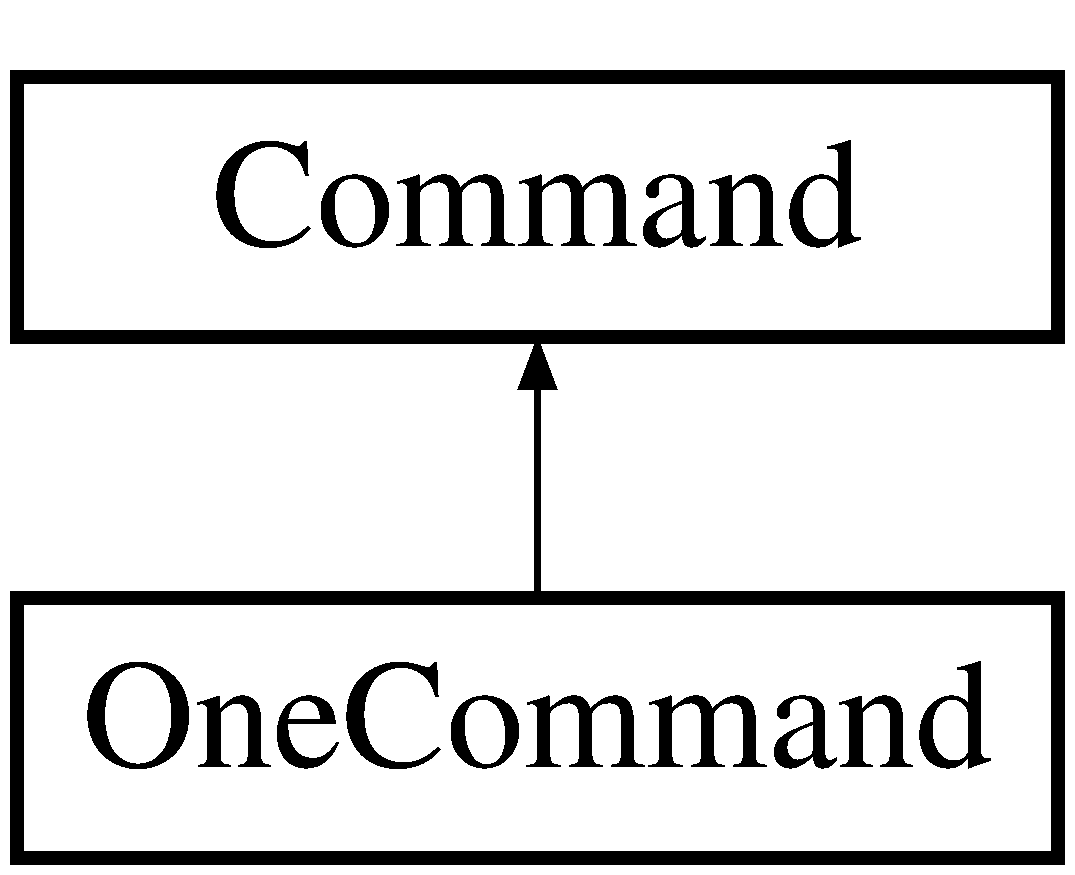
\includegraphics[height=2.000000cm]{class_one_command}
\end{center}
\end{figure}
\subsection*{Public Member Functions}
\begin{DoxyCompactItemize}
\item 
\hyperlink{class_one_command_a20db00d94b5c1d86603be7d91fcd0303}{One\+Command} (Calculator $\ast$new\+Calc)
\begin{DoxyCompactList}\small\item\em A constructor. Sets pointer to the implementation of. \end{DoxyCompactList}\item 
\hyperlink{class_one_command_a0e27a8696729eee5f0e0e399519b2237}{$\sim$\+One\+Command} ()
\item 
void \hyperlink{class_one_command_a5a044d694cd01f447d1f57ac25dccd01}{execute} ()
\begin{DoxyCompactList}\small\item\em Executes diving command of. \end{DoxyCompactList}\end{DoxyCompactItemize}
\subsection*{Public Attributes}
\begin{DoxyCompactItemize}
\item 
Calculator $\ast$ \hyperlink{class_one_command_a8867d5fb2fd62bfcd2a7d9f69bf08d93}{calculator}
\end{DoxyCompactItemize}


\subsection{Detailed Description}
implementations of one command 

Calculator -\/ Simple calculator realization by patterns Copyright (C) 2017 -\/ ? Alexey Konyshev (\href{mailto:aleksey.konyshev@gmail.com}{\tt aleksey.\+konyshev@gmail.\+com})

This software is provided \textquotesingle{}as-\/is\textquotesingle{}, without any express or implied warranty. In no event will the authors be held liable for any damages arising from the use of this software.

Permission is granted to anyone to use this software for any purpose, including commercial applications, and to alter it and redistribute it freely, subject to the following restrictions\+:


\begin{DoxyEnumerate}
\item The origin of this software must not be misrepresented; you must not claim that you wrote the original software. If you use this software in a product, an acknowledgment in the product documentation would be appreciated but is not required.
\item Altered source versions must be plainly marked as such, and must not be misrepresented as being the original software.
\item This notice may not be removed or altered from any source distribution. Headers 
\begin{DoxyCode}
\hyperlink{class_command}{Command} 
\end{DoxyCode}
 
\end{DoxyEnumerate}

\subsection{Constructor \& Destructor Documentation}
\hypertarget{class_one_command_a20db00d94b5c1d86603be7d91fcd0303}{}\index{One\+Command@{One\+Command}!One\+Command@{One\+Command}}
\index{One\+Command@{One\+Command}!One\+Command@{One\+Command}}
\subsubsection[{One\+Command(\+Calculator $\ast$new\+Calc)}]{\setlength{\rightskip}{0pt plus 5cm}One\+Command\+::\+One\+Command (
\begin{DoxyParamCaption}
\item[{Calculator $\ast$}]{new\+Calc}
\end{DoxyParamCaption}
)}\label{class_one_command_a20db00d94b5c1d86603be7d91fcd0303}


A constructor. Sets pointer to the implementation of. 


\begin{DoxyCode}
Calculator 
\end{DoxyCode}



\begin{DoxyParams}{Parameters}
{\em new\+Calc} & a new
\begin{DoxyCode}
Calculator 
\end{DoxyCode}
\\
\hline
\end{DoxyParams}
Calculator -\/ Simple calculator realization by patterns Copyright (C) 2017 -\/ ? Alexey Konyshev (\href{mailto:aleksey.konyshev@gmail.com}{\tt aleksey.\+konyshev@gmail.\+com})

This software is provided \textquotesingle{}as-\/is\textquotesingle{}, without any express or implied warranty. In no event will the authors be held liable for any damages arising from the use of this software.

Permission is granted to anyone to use this software for any purpose, including commercial applications, and to alter it and redistribute it freely, subject to the following restrictions\+:


\begin{DoxyEnumerate}
\item The origin of this software must not be misrepresented; you must not claim that you wrote the original software. If you use this software in a product, an acknowledgment in the product documentation would be appreciated but is not required.
\item Altered source versions must be plainly marked as such, and must not be misrepresented as being the original software.
\item This notice may not be removed or altered from any source distribution. Headers 
\end{DoxyEnumerate}\hypertarget{class_one_command_a0e27a8696729eee5f0e0e399519b2237}{}\index{One\+Command@{One\+Command}!````~One\+Command@{$\sim$\+One\+Command}}
\index{````~One\+Command@{$\sim$\+One\+Command}!One\+Command@{One\+Command}}
\subsubsection[{$\sim$\+One\+Command()}]{\setlength{\rightskip}{0pt plus 5cm}One\+Command\+::$\sim$\+One\+Command (
\begin{DoxyParamCaption}
{}
\end{DoxyParamCaption}
)}\label{class_one_command_a0e27a8696729eee5f0e0e399519b2237}
A destructor 

\subsection{Member Function Documentation}
\hypertarget{class_one_command_a5a044d694cd01f447d1f57ac25dccd01}{}\index{One\+Command@{One\+Command}!execute@{execute}}
\index{execute@{execute}!One\+Command@{One\+Command}}
\subsubsection[{execute()}]{\setlength{\rightskip}{0pt plus 5cm}void One\+Command\+::execute (
\begin{DoxyParamCaption}
{}
\end{DoxyParamCaption}
)\hspace{0.3cm}{\ttfamily [virtual]}}\label{class_one_command_a5a044d694cd01f447d1f57ac25dccd01}


Executes diving command of. 


\begin{DoxyCode}
Calculator 
\end{DoxyCode}
 

Implements \hyperlink{class_command_a6fd7d9bd8df8bfc881e4d6c7cd1878b7}{Command}.



\subsection{Member Data Documentation}
\hypertarget{class_one_command_a8867d5fb2fd62bfcd2a7d9f69bf08d93}{}\index{One\+Command@{One\+Command}!calculator@{calculator}}
\index{calculator@{calculator}!One\+Command@{One\+Command}}
\subsubsection[{calculator}]{\setlength{\rightskip}{0pt plus 5cm}Calculator$\ast$ One\+Command\+::calculator}\label{class_one_command_a8867d5fb2fd62bfcd2a7d9f69bf08d93}
pointer to the
\begin{DoxyCode}
Calculator 
\end{DoxyCode}
 

The documentation for this class was generated from the following files\+:\begin{DoxyCompactItemize}
\item 
One\+Command.\+h\item 
One\+Command.\+cpp\end{DoxyCompactItemize}

\hypertarget{class_plus_command}{}\section{Plus\+Command Class Reference}
\label{class_plus_command}\index{Plus\+Command@{Plus\+Command}}
Inheritance diagram for Plus\+Command\+:\begin{figure}[H]
\begin{center}
\leavevmode
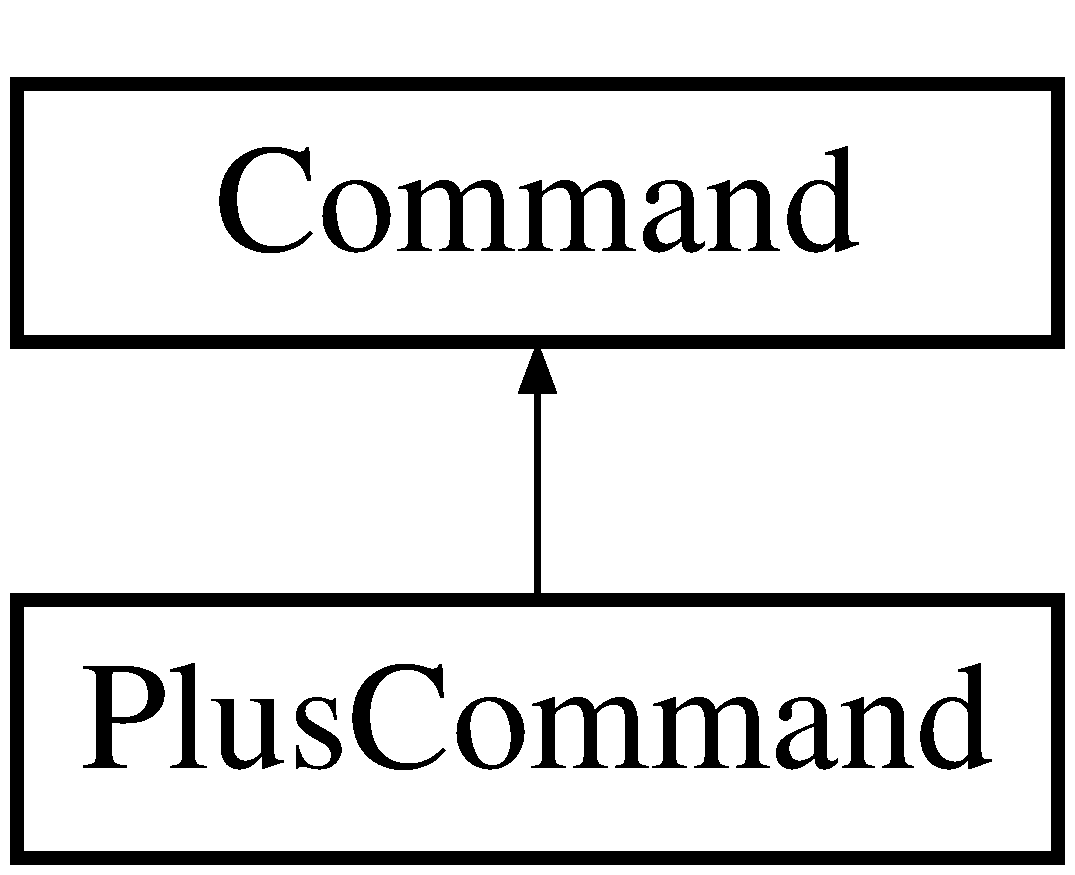
\includegraphics[height=2.000000cm]{class_plus_command}
\end{center}
\end{figure}
\subsection*{Public Member Functions}
\begin{DoxyCompactItemize}
\item 
\hypertarget{class_plus_command_a687cab12cc701d06dcf998c42c30bc31}{}{\bfseries Plus\+Command} (\hyperlink{class_calculator}{Calculator} $\ast$new\+Calc)\label{class_plus_command_a687cab12cc701d06dcf998c42c30bc31}

\item 
\hypertarget{class_plus_command_a43c95e8e8ac4260f507f92d9d40f0699}{}void \hyperlink{class_plus_command_a43c95e8e8ac4260f507f92d9d40f0699}{execute} ()\label{class_plus_command_a43c95e8e8ac4260f507f92d9d40f0699}

\begin{DoxyCompactList}\small\item\em Executes some functionality in buisness logic. \end{DoxyCompactList}\end{DoxyCompactItemize}
\subsection*{Public Attributes}
\begin{DoxyCompactItemize}
\item 
\hypertarget{class_plus_command_a6dd3da59e837ac5bcd1063ecc5895f0e}{}\hyperlink{class_calculator}{Calculator} $\ast$ {\bfseries calculator}\label{class_plus_command_a6dd3da59e837ac5bcd1063ecc5895f0e}

\end{DoxyCompactItemize}


The documentation for this class was generated from the following files\+:\begin{DoxyCompactItemize}
\item 
Plus\+Command.\+h\item 
Plus\+Command.\+cpp\end{DoxyCompactItemize}

\hypertarget{class_plus_math_op}{}\section{Plus\+Math\+Op Class Reference}
\label{class_plus_math_op}\index{Plus\+Math\+Op@{Plus\+Math\+Op}}


{\ttfamily \#include $<$Plus\+Math\+Op.\+h$>$}

Inheritance diagram for Plus\+Math\+Op\+:\begin{figure}[H]
\begin{center}
\leavevmode
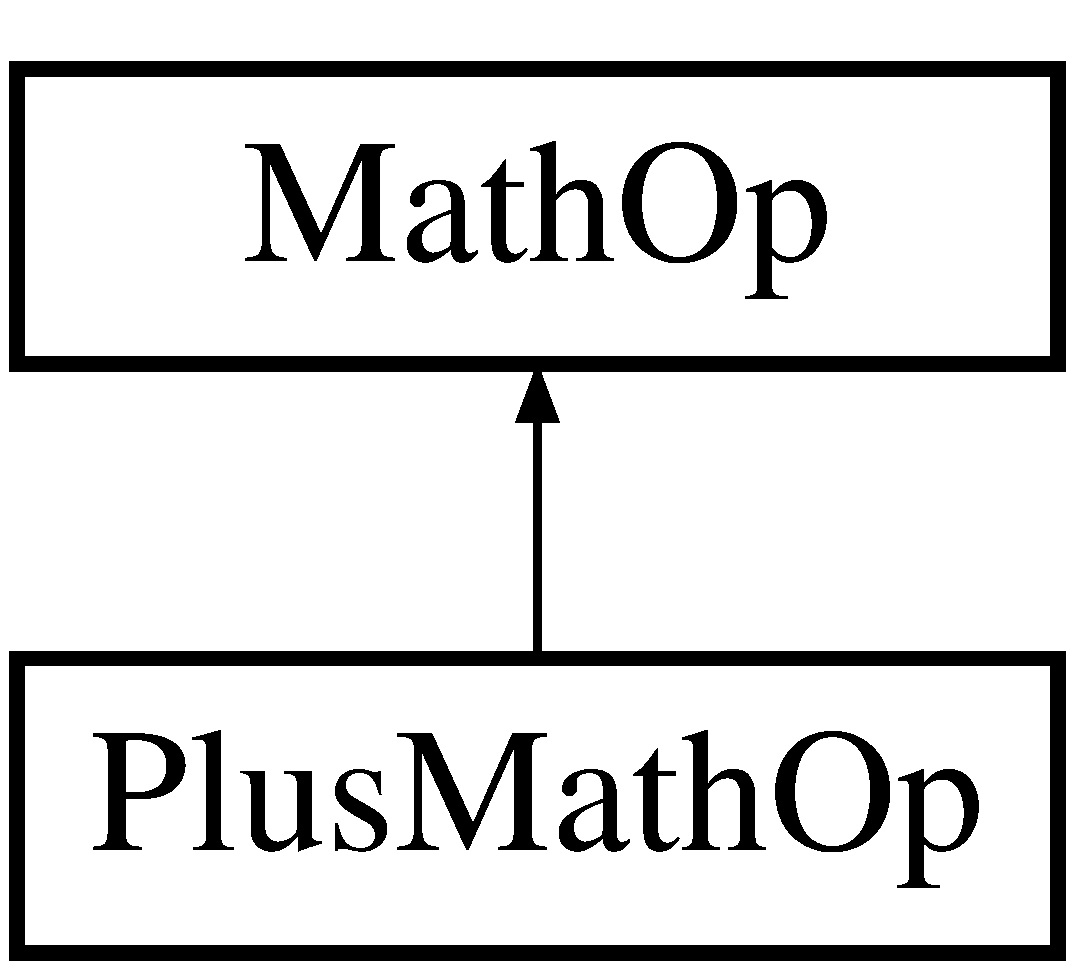
\includegraphics[height=2.000000cm]{class_plus_math_op}
\end{center}
\end{figure}
\subsection*{Public Member Functions}
\begin{DoxyCompactItemize}
\item 
\hyperlink{class_plus_math_op_a6c6a14c9b1b9a4078d23e9ebe1b0d9d3}{Plus\+Math\+Op} ()
\item 
\hypertarget{class_plus_math_op_af4a0c7be45556dc4c7c78011626ede7b}{}void {\bfseries execute} ()\label{class_plus_math_op_af4a0c7be45556dc4c7c78011626ede7b}

\end{DoxyCompactItemize}
\subsection*{Additional Inherited Members}


\subsection{Detailed Description}
Calculator -\/ Simple calculator realization by patterns Copyright (C) 2017 -\/ ? Alexey Konyshev (\href{mailto:aleksey.konyshev@gmail.com}{\tt aleksey.\+konyshev@gmail.\+com})

This software is provided \textquotesingle{}as-\/is\textquotesingle{}, without any express or implied warranty. In no event will the authors be held liable for any damages arising from the use of this software.

Permission is granted to anyone to use this software for any purpose, including commercial applications, and to alter it and redistribute it freely, subject to the following restrictions\+:


\begin{DoxyEnumerate}
\item The origin of this software must not be misrepresented; you must not claim that you wrote the original software. If you use this software in a product, an acknowledgment in the product documentation would be appreciated but is not required.
\item Altered source versions must be plainly marked as such, and must not be misrepresented as being the original software.
\item This notice may not be removed or altered from any source distribution. 
\end{DoxyEnumerate}

\subsection{Constructor \& Destructor Documentation}
\hypertarget{class_plus_math_op_a6c6a14c9b1b9a4078d23e9ebe1b0d9d3}{}\index{Plus\+Math\+Op@{Plus\+Math\+Op}!Plus\+Math\+Op@{Plus\+Math\+Op}}
\index{Plus\+Math\+Op@{Plus\+Math\+Op}!Plus\+Math\+Op@{Plus\+Math\+Op}}
\subsubsection[{Plus\+Math\+Op()}]{\setlength{\rightskip}{0pt plus 5cm}Plus\+Math\+Op\+::\+Plus\+Math\+Op (
\begin{DoxyParamCaption}
{}
\end{DoxyParamCaption}
)}\label{class_plus_math_op_a6c6a14c9b1b9a4078d23e9ebe1b0d9d3}
Calculator -\/ Simple calculator realization by patterns Copyright (C) 2017 -\/ ? Alexey Konyshev (\href{mailto:aleksey.konyshev@gmail.com}{\tt aleksey.\+konyshev@gmail.\+com})

This software is provided \textquotesingle{}as-\/is\textquotesingle{}, without any express or implied warranty. In no event will the authors be held liable for any damages arising from the use of this software.

Permission is granted to anyone to use this software for any purpose, including commercial applications, and to alter it and redistribute it freely, subject to the following restrictions\+:


\begin{DoxyEnumerate}
\item The origin of this software must not be misrepresented; you must not claim that you wrote the original software. If you use this software in a product, an acknowledgment in the product documentation would be appreciated but is not required.
\item Altered source versions must be plainly marked as such, and must not be misrepresented as being the original software.
\item This notice may not be removed or altered from any source distribution. Headers 
\end{DoxyEnumerate}

The documentation for this class was generated from the following files\+:\begin{DoxyCompactItemize}
\item 
Plus\+Math\+Op.\+h\item 
Plus\+Math\+Op.\+cpp\end{DoxyCompactItemize}

\hypertarget{class_point_command}{}\section{Point\+Command Class Reference}
\label{class_point_command}\index{Point\+Command@{Point\+Command}}
Inheritance diagram for Point\+Command\+:\begin{figure}[H]
\begin{center}
\leavevmode
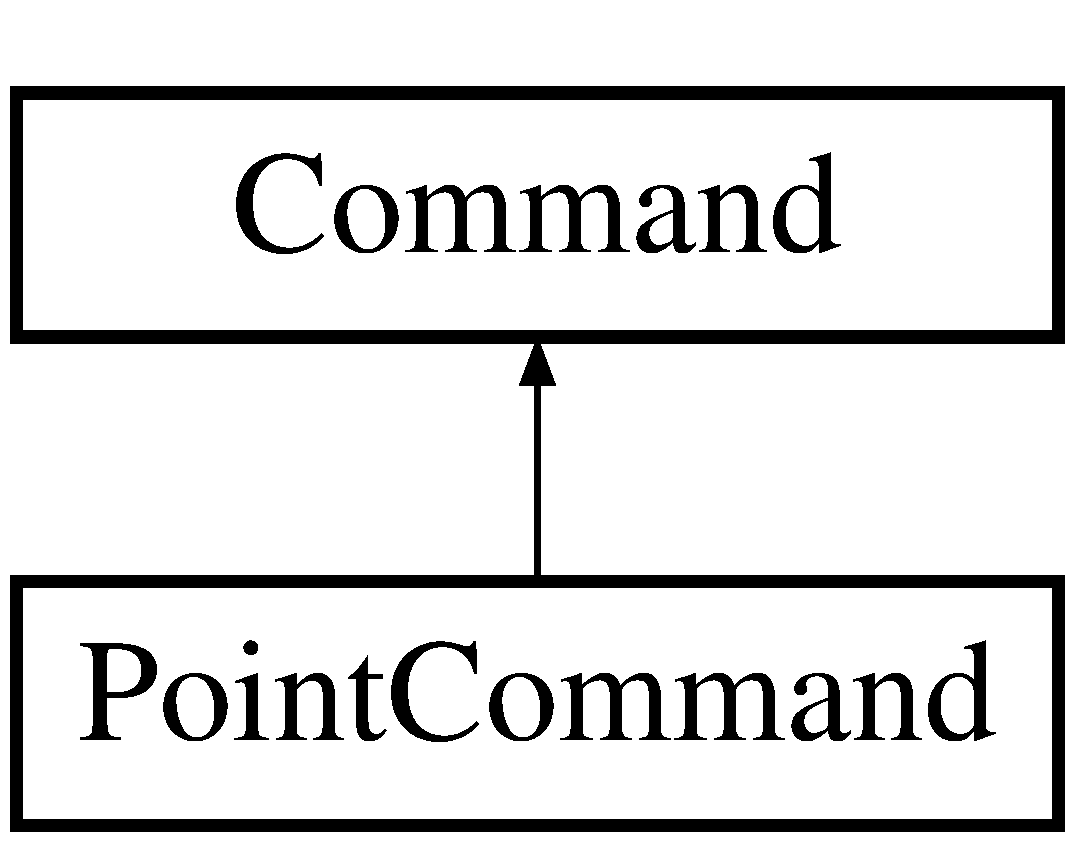
\includegraphics[height=2.000000cm]{class_point_command}
\end{center}
\end{figure}
\subsection*{Public Member Functions}
\begin{DoxyCompactItemize}
\item 
\hypertarget{class_point_command_acc022d8812e9d289bf723dd900a338bb}{}{\bfseries Point\+Command} (\hyperlink{class_calculator}{Calculator} $\ast$new\+Calc)\label{class_point_command_acc022d8812e9d289bf723dd900a338bb}

\item 
\hypertarget{class_point_command_a681f8465afa18959cd268fab140d9f69}{}void \hyperlink{class_point_command_a681f8465afa18959cd268fab140d9f69}{execute} ()\label{class_point_command_a681f8465afa18959cd268fab140d9f69}

\begin{DoxyCompactList}\small\item\em Executes some functionality in buisness logic. \end{DoxyCompactList}\end{DoxyCompactItemize}
\subsection*{Public Attributes}
\begin{DoxyCompactItemize}
\item 
\hypertarget{class_point_command_a63132439ae2e59216eddddd4754f9109}{}\hyperlink{class_calculator}{Calculator} $\ast$ {\bfseries calculator}\label{class_point_command_a63132439ae2e59216eddddd4754f9109}

\end{DoxyCompactItemize}


The documentation for this class was generated from the following files\+:\begin{DoxyCompactItemize}
\item 
Point\+Command.\+h\item 
Point\+Command.\+cpp\end{DoxyCompactItemize}

\hypertarget{class_screen}{}\section{Screen Class Reference}
\label{class_screen}\index{Screen@{Screen}}


{\ttfamily \#include $<$Screen.\+h$>$}

Inheritance diagram for Screen\+:\begin{figure}[H]
\begin{center}
\leavevmode
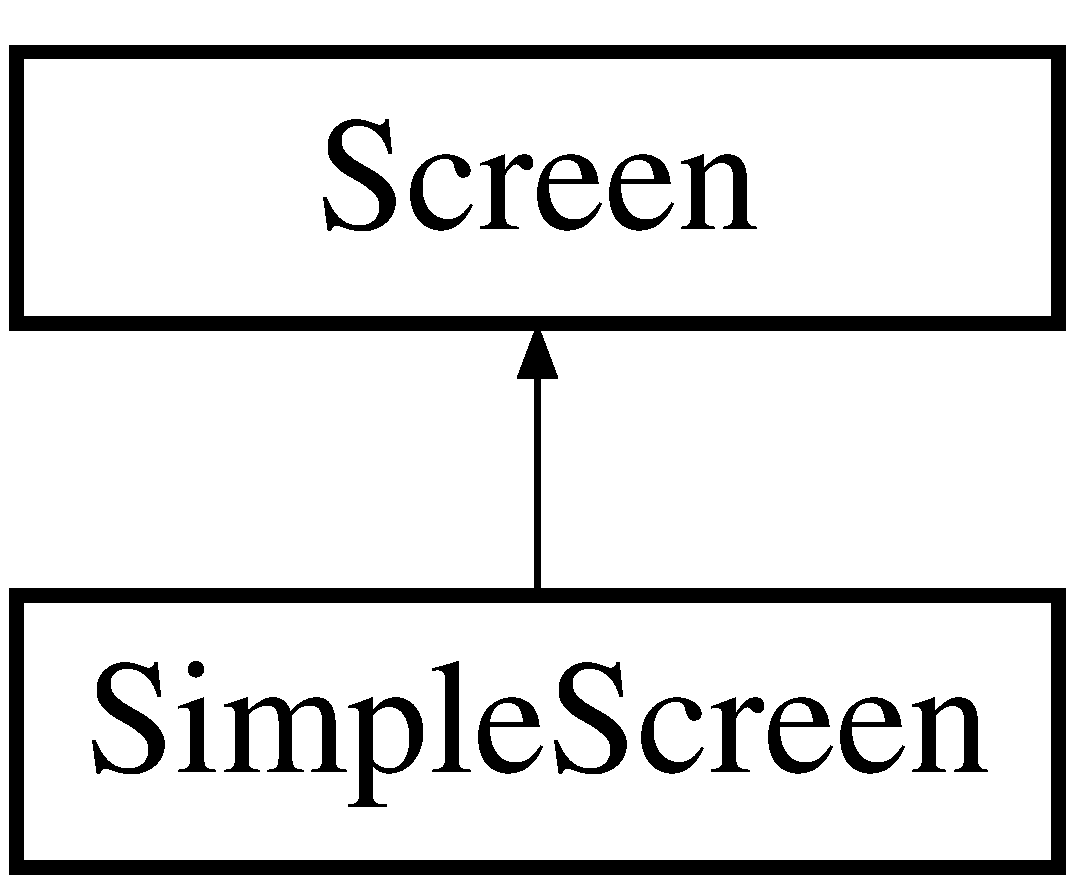
\includegraphics[height=2.000000cm]{class_screen}
\end{center}
\end{figure}
\subsection*{Public Member Functions}
\begin{DoxyCompactItemize}
\item 
void \hyperlink{class_screen_a77de1ee1d98d21bb8bab21e9f507c369}{set\+State} (\hyperlink{class_screen_state}{Screen\+State} $\ast$new\+Screen\+Statew)
\item 
void \hyperlink{class_screen_a43f495857effafe04848a91dfc229fbe}{type\+Symbol} (std\+::string new\+Symbol)
\begin{DoxyCompactList}\small\item\em adds new symbol to the screan \end{DoxyCompactList}\item 
std\+::string \hyperlink{class_screen_a82445b0bebdac598ab96fecdd362e387}{get\+Screen} ()
\begin{DoxyCompactList}\small\item\em get current value of screan \end{DoxyCompactList}\item 
\hypertarget{class_screen_ab8f41de38bab8a2a16eb40fb66af00f2}{}void \hyperlink{class_screen_ab8f41de38bab8a2a16eb40fb66af00f2}{clear\+Screen} ()\label{class_screen_ab8f41de38bab8a2a16eb40fb66af00f2}

\begin{DoxyCompactList}\small\item\em Clear screan variable and set size 0. \end{DoxyCompactList}\item 
\hypertarget{class_screen_a1ab0cbcdffb9e088ee5439d0bea82d2f}{}void {\bfseries type\+Double} (double value)\label{class_screen_a1ab0cbcdffb9e088ee5439d0bea82d2f}

\end{DoxyCompactItemize}
\subsection*{Public Attributes}
\begin{DoxyCompactItemize}
\item 
\hypertarget{class_screen_a027afe6f31862a0a06bd785538f30558}{}std\+::stringstream {\bfseries ss}\label{class_screen_a027afe6f31862a0a06bd785538f30558}

\item 
\hypertarget{class_screen_afc44809d98c65830d23ec33acb1fdb1f}{}int {\bfseries size}\label{class_screen_afc44809d98c65830d23ec33acb1fdb1f}

\item 
\hypertarget{class_screen_a4e6d87519cee816a2b3bff3bf679c714}{}\hyperlink{class_screen_state}{Screen\+State} $\ast$ {\bfseries state}\label{class_screen_a4e6d87519cee816a2b3bff3bf679c714}

\end{DoxyCompactItemize}


\subsection{Detailed Description}
Calculator -\/ Simple calculator realization by patterns Copyright (C) 2017 -\/ ? Alexey Konyshev (\href{mailto:aleksey.konyshev@gmail.com}{\tt aleksey.\+konyshev@gmail.\+com})

This software is provided \textquotesingle{}as-\/is\textquotesingle{}, without any express or implied warranty. In no event will the authors be held liable for any damages arising from the use of this software.

Permission is granted to anyone to use this software for any purpose, including commercial applications, and to alter it and redistribute it freely, subject to the following restrictions\+:


\begin{DoxyEnumerate}
\item The origin of this software must not be misrepresented; you must not claim that you wrote the original software. If you use this software in a product, an acknowledgment in the product documentation would be appreciated but is not required.
\item Altered source versions must be plainly marked as such, and must not be misrepresented as being the original software.
\item This notice may not be removed or altered from any source distribution. 
\end{DoxyEnumerate}

\subsection{Member Function Documentation}
\hypertarget{class_screen_a82445b0bebdac598ab96fecdd362e387}{}\index{Screen@{Screen}!get\+Screen@{get\+Screen}}
\index{get\+Screen@{get\+Screen}!Screen@{Screen}}
\subsubsection[{get\+Screen()}]{\setlength{\rightskip}{0pt plus 5cm}std\+::string Screen\+::get\+Screen (
\begin{DoxyParamCaption}
{}
\end{DoxyParamCaption}
)}\label{class_screen_a82445b0bebdac598ab96fecdd362e387}


get current value of screan 

\begin{DoxyReturn}{Returns}
screan 
\end{DoxyReturn}
\hypertarget{class_screen_a77de1ee1d98d21bb8bab21e9f507c369}{}\index{Screen@{Screen}!set\+State@{set\+State}}
\index{set\+State@{set\+State}!Screen@{Screen}}
\subsubsection[{set\+State(\+Screen\+State $\ast$new\+Screen\+Statew)}]{\setlength{\rightskip}{0pt plus 5cm}void Screen\+::set\+State (
\begin{DoxyParamCaption}
\item[{{\bf Screen\+State} $\ast$}]{new\+Screen\+Statew}
\end{DoxyParamCaption}
)}\label{class_screen_a77de1ee1d98d21bb8bab21e9f507c369}
Calculator -\/ Simple calculator realization by patterns Copyright (C) 2017 -\/ ? Alexey Konyshev (\href{mailto:aleksey.konyshev@gmail.com}{\tt aleksey.\+konyshev@gmail.\+com})

This software is provided \textquotesingle{}as-\/is\textquotesingle{}, without any express or implied warranty. In no event will the authors be held liable for any damages arising from the use of this software.

Permission is granted to anyone to use this software for any purpose, including commercial applications, and to alter it and redistribute it freely, subject to the following restrictions\+:


\begin{DoxyEnumerate}
\item The origin of this software must not be misrepresented; you must not claim that you wrote the original software. If you use this software in a product, an acknowledgment in the product documentation would be appreciated but is not required.
\item Altered source versions must be plainly marked as such, and must not be misrepresented as being the original software.
\item This notice may not be removed or altered from any source distribution. 
\end{DoxyEnumerate}\hypertarget{class_screen_a43f495857effafe04848a91dfc229fbe}{}\index{Screen@{Screen}!type\+Symbol@{type\+Symbol}}
\index{type\+Symbol@{type\+Symbol}!Screen@{Screen}}
\subsubsection[{type\+Symbol(std\+::string new\+Symbol)}]{\setlength{\rightskip}{0pt plus 5cm}void Screen\+::type\+Symbol (
\begin{DoxyParamCaption}
\item[{std\+::string}]{new\+Symbol}
\end{DoxyParamCaption}
)}\label{class_screen_a43f495857effafe04848a91dfc229fbe}


adds new symbol to the screan 


\begin{DoxyParams}{Parameters}
{\em new\+Symbol} & \\
\hline
\end{DoxyParams}


The documentation for this class was generated from the following files\+:\begin{DoxyCompactItemize}
\item 
Screen.\+h\item 
Screen.\+cpp\end{DoxyCompactItemize}

\hypertarget{class_screen_state}{}\section{Screen\+State Class Reference}
\label{class_screen_state}\index{Screen\+State@{Screen\+State}}


{\ttfamily \#include $<$Screen\+State.\+h$>$}

Inheritance diagram for Screen\+State\+:\begin{figure}[H]
\begin{center}
\leavevmode
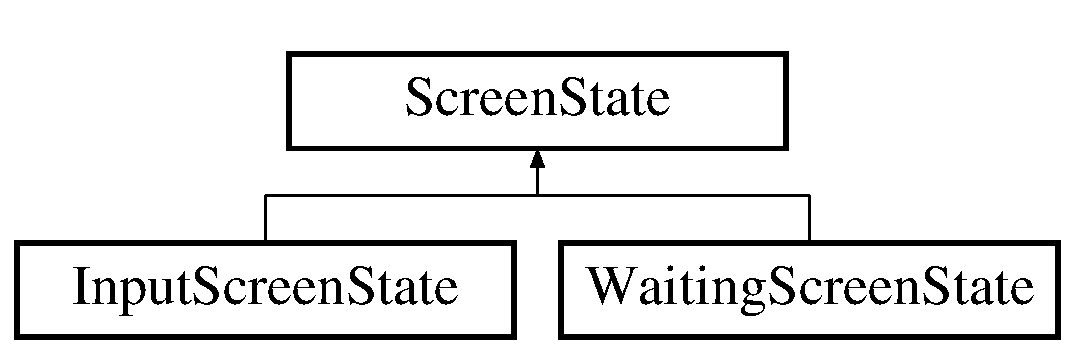
\includegraphics[height=2.000000cm]{class_screen_state}
\end{center}
\end{figure}
\subsection*{Public Member Functions}
\begin{DoxyCompactItemize}
\item 
virtual void \hyperlink{class_screen_state_adb71081141ec6c066d54f1dc77c78717}{input} (std\+::string new\+Symbol)=0
\begin{DoxyCompactList}\small\item\em Input new symbol to the screan according current state. \end{DoxyCompactList}\item 
\hypertarget{class_screen_state_a7ed07cbc56ad6b472263a6035335ad95}{}virtual void \hyperlink{class_screen_state_a7ed07cbc56ad6b472263a6035335ad95}{clear} ()=0\label{class_screen_state_a7ed07cbc56ad6b472263a6035335ad95}

\begin{DoxyCompactList}\small\item\em Clear screen according state. \end{DoxyCompactList}\end{DoxyCompactItemize}


\subsection{Detailed Description}
Calculator -\/ Simple calculator realization by patterns Copyright (C) 2017 -\/ ? Alexey Konyshev (\href{mailto:aleksey.konyshev@gmail.com}{\tt aleksey.\+konyshev@gmail.\+com})

This software is provided \textquotesingle{}as-\/is\textquotesingle{}, without any express or implied warranty. In no event will the authors be held liable for any damages arising from the use of this software.

Permission is granted to anyone to use this software for any purpose, including commercial applications, and to alter it and redistribute it freely, subject to the following restrictions\+:


\begin{DoxyEnumerate}
\item The origin of this software must not be misrepresented; you must not claim that you wrote the original software. If you use this software in a product, an acknowledgment in the product documentation would be appreciated but is not required.
\item Altered source versions must be plainly marked as such, and must not be misrepresented as being the original software.
\item This notice may not be removed or altered from any source distribution. 
\end{DoxyEnumerate}

\subsection{Member Function Documentation}
\hypertarget{class_screen_state_adb71081141ec6c066d54f1dc77c78717}{}\index{Screen\+State@{Screen\+State}!input@{input}}
\index{input@{input}!Screen\+State@{Screen\+State}}
\subsubsection[{input(std\+::string new\+Symbol)=0}]{\setlength{\rightskip}{0pt plus 5cm}virtual void Screen\+State\+::input (
\begin{DoxyParamCaption}
\item[{std\+::string}]{new\+Symbol}
\end{DoxyParamCaption}
)\hspace{0.3cm}{\ttfamily [pure virtual]}}\label{class_screen_state_adb71081141ec6c066d54f1dc77c78717}


Input new symbol to the screan according current state. 


\begin{DoxyParams}{Parameters}
{\em new\+Symbol} & \\
\hline
\end{DoxyParams}


Implemented in \hyperlink{class_waiting_screen_state_ac22e314bd11df4ba4d5480da022f5862}{Waiting\+Screen\+State}, and \hyperlink{class_input_screen_state_a2189d602f5fe02660488a5a49c4c76f8}{Input\+Screen\+State}.



The documentation for this class was generated from the following file\+:\begin{DoxyCompactItemize}
\item 
Screen\+State.\+h\end{DoxyCompactItemize}

\hypertarget{class_seven_command}{}\section{Seven\+Command Class Reference}
\label{class_seven_command}\index{Seven\+Command@{Seven\+Command}}
Inheritance diagram for Seven\+Command\+:\begin{figure}[H]
\begin{center}
\leavevmode
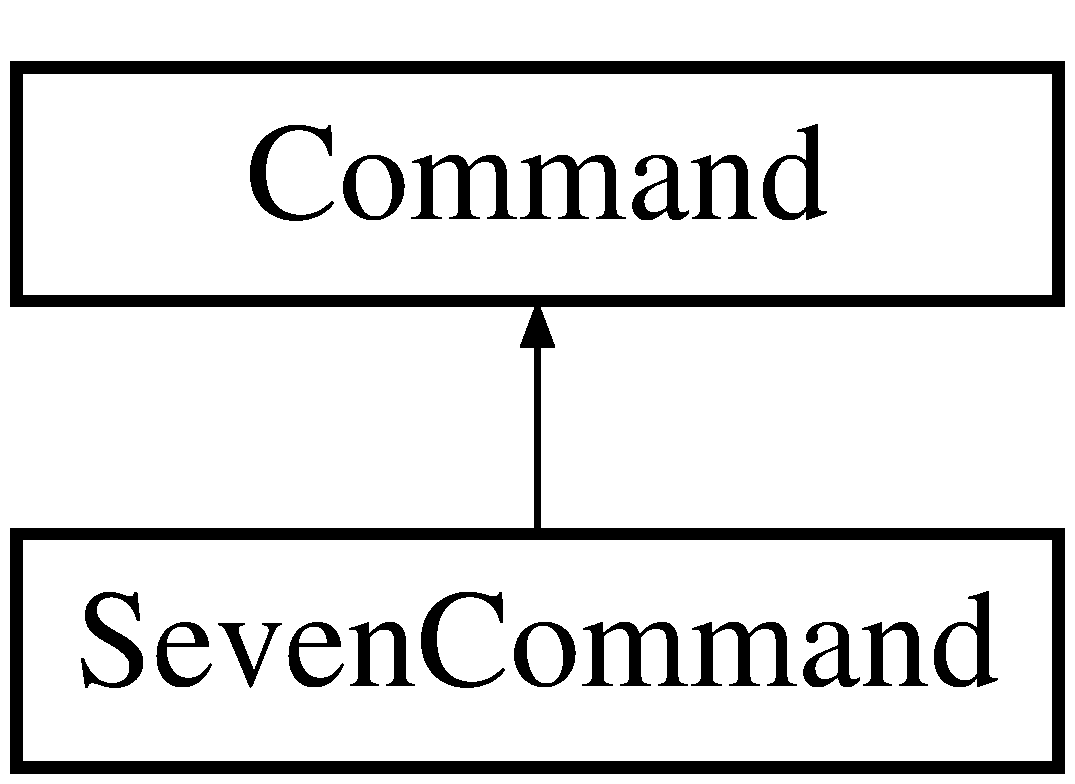
\includegraphics[height=2.000000cm]{class_seven_command}
\end{center}
\end{figure}
\subsection*{Public Member Functions}
\begin{DoxyCompactItemize}
\item 
\hypertarget{class_seven_command_a0b3849d60dc9d685e42bc9791a28a1cd}{}{\bfseries Seven\+Command} (\hyperlink{class_calculator}{Calculator} $\ast$new\+Calc)\label{class_seven_command_a0b3849d60dc9d685e42bc9791a28a1cd}

\item 
\hypertarget{class_seven_command_a89ebb0bc60979b8b6d5dc65cc195f38f}{}void {\bfseries execute} ()\label{class_seven_command_a89ebb0bc60979b8b6d5dc65cc195f38f}

\end{DoxyCompactItemize}
\subsection*{Public Attributes}
\begin{DoxyCompactItemize}
\item 
\hypertarget{class_seven_command_a5758d5e5b5981f81bd56c54c87f25b48}{}\hyperlink{class_calculator}{Calculator} $\ast$ {\bfseries calculator}\label{class_seven_command_a5758d5e5b5981f81bd56c54c87f25b48}

\end{DoxyCompactItemize}


The documentation for this class was generated from the following files\+:\begin{DoxyCompactItemize}
\item 
Seven\+Command.\+h\item 
Seven\+Command.\+cpp\end{DoxyCompactItemize}

\hypertarget{class_simple_calculator}{}\section{Simple\+Calculator Class Reference}
\label{class_simple_calculator}\index{Simple\+Calculator@{Simple\+Calculator}}


{\ttfamily \#include $<$Simple\+Calculator.\+h$>$}

Inheritance diagram for Simple\+Calculator\+:\begin{figure}[H]
\begin{center}
\leavevmode
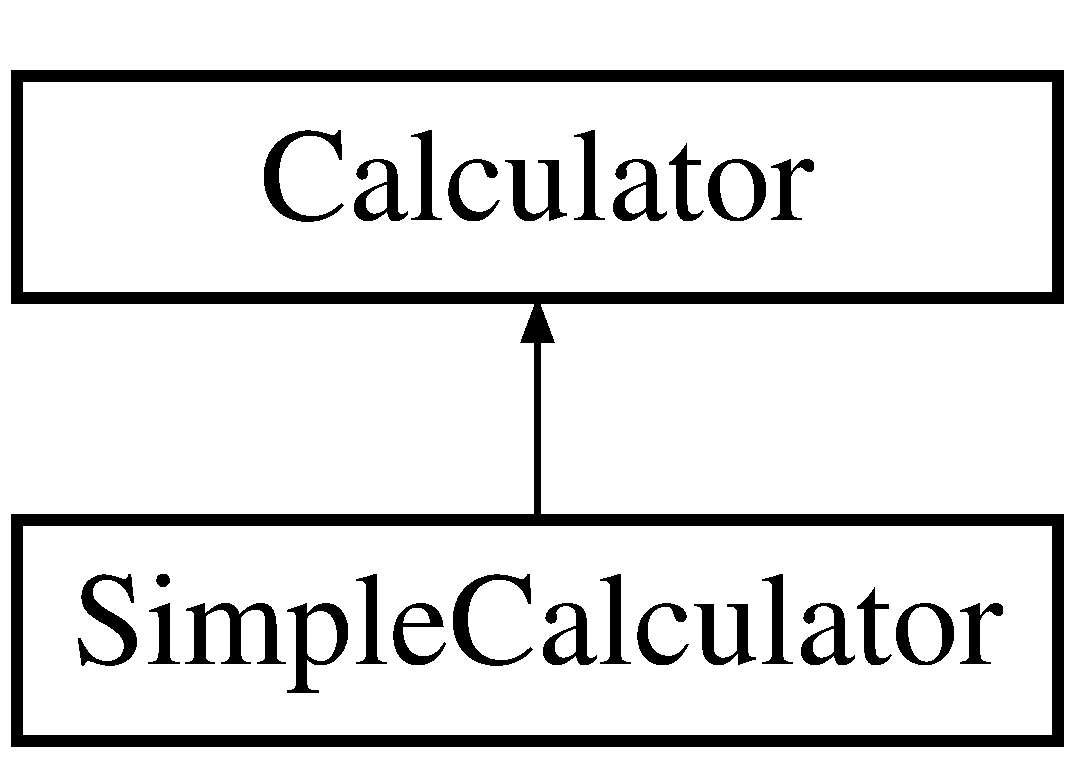
\includegraphics[height=2.000000cm]{class_simple_calculator}
\end{center}
\end{figure}
\subsection*{Public Member Functions}
\begin{DoxyCompactItemize}
\item 
\hyperlink{class_simple_calculator_abc3dbc4a359f61839604243111076ad0}{Simple\+Calculator} ()
\item 
\hypertarget{class_simple_calculator_aa3bd09c9f5110a03974370f40e5730b2}{}void {\bfseries One} ()\label{class_simple_calculator_aa3bd09c9f5110a03974370f40e5730b2}

\item 
\hypertarget{class_simple_calculator_aa86e716cba419eab04d54bf6c81813ed}{}void {\bfseries Two} ()\label{class_simple_calculator_aa86e716cba419eab04d54bf6c81813ed}

\item 
\hypertarget{class_simple_calculator_a04d7cbe2f81cc153d7d3585d419748eb}{}void {\bfseries Three} ()\label{class_simple_calculator_a04d7cbe2f81cc153d7d3585d419748eb}

\item 
\hypertarget{class_simple_calculator_a9ac1a3907ac92d44023377d0092c338c}{}void {\bfseries Four} ()\label{class_simple_calculator_a9ac1a3907ac92d44023377d0092c338c}

\item 
\hypertarget{class_simple_calculator_a7f6caf82ea486dfedb07d7255086958c}{}void {\bfseries Five} ()\label{class_simple_calculator_a7f6caf82ea486dfedb07d7255086958c}

\item 
\hypertarget{class_simple_calculator_a39da478b7dc5da6ea463851de861be8b}{}void {\bfseries Six} ()\label{class_simple_calculator_a39da478b7dc5da6ea463851de861be8b}

\item 
\hypertarget{class_simple_calculator_ab7e9de1426acd6994ad9ba410171a2ab}{}void {\bfseries Seven} ()\label{class_simple_calculator_ab7e9de1426acd6994ad9ba410171a2ab}

\item 
\hypertarget{class_simple_calculator_a112c39b663a0666b47131d929fc14943}{}void {\bfseries Eight} ()\label{class_simple_calculator_a112c39b663a0666b47131d929fc14943}

\item 
\hypertarget{class_simple_calculator_a17494a987cba00cfa6af6cfecd379ee5}{}void {\bfseries Nine} ()\label{class_simple_calculator_a17494a987cba00cfa6af6cfecd379ee5}

\item 
\hypertarget{class_simple_calculator_a976544f13100e0d2f9b426e498cefbaf}{}void {\bfseries Zero} ()\label{class_simple_calculator_a976544f13100e0d2f9b426e498cefbaf}

\item 
\hypertarget{class_simple_calculator_a1c3d98efd260d24257c1f6d191c1c49b}{}void {\bfseries Plus} ()\label{class_simple_calculator_a1c3d98efd260d24257c1f6d191c1c49b}

\item 
\hypertarget{class_simple_calculator_a7fa56beb68f4106117c42a79938c09eb}{}void {\bfseries Minus} ()\label{class_simple_calculator_a7fa56beb68f4106117c42a79938c09eb}

\item 
\hypertarget{class_simple_calculator_a9b2934538c26e04415e7e0f72292429f}{}void {\bfseries Mul} ()\label{class_simple_calculator_a9b2934538c26e04415e7e0f72292429f}

\item 
\hypertarget{class_simple_calculator_a42c605ac8def4b8736044823397dded3}{}void {\bfseries Div} ()\label{class_simple_calculator_a42c605ac8def4b8736044823397dded3}

\item 
\hypertarget{class_simple_calculator_a6e500a4a9894645611443efb54384739}{}void {\bfseries Point} ()\label{class_simple_calculator_a6e500a4a9894645611443efb54384739}

\item 
\hypertarget{class_simple_calculator_ac761197c4fb7e81f36c7eb148e505747}{}void {\bfseries Enter} ()\label{class_simple_calculator_ac761197c4fb7e81f36c7eb148e505747}

\item 
\hypertarget{class_simple_calculator_a0d1f0a06695738d8b4f64e04c7e894cb}{}void {\bfseries Undo} ()\label{class_simple_calculator_a0d1f0a06695738d8b4f64e04c7e894cb}

\item 
\hypertarget{class_simple_calculator_ab6ace836623e75cc2c9150d9b648804d}{}double {\bfseries get\+Result} ()\label{class_simple_calculator_ab6ace836623e75cc2c9150d9b648804d}

\end{DoxyCompactItemize}
\subsection*{Public Attributes}
\begin{DoxyCompactItemize}
\item 
\hypertarget{class_simple_calculator_a4d8d30bd990c0d203281bae710467047}{}\hyperlink{class_plus_math_op}{Plus\+Math\+Op} {\bfseries plus\+Op}\label{class_simple_calculator_a4d8d30bd990c0d203281bae710467047}

\item 
\hypertarget{class_simple_calculator_a5040eae51fb4c48586355e7eb32e1351}{}\hyperlink{class_minus_math_op}{Minus\+Math\+Op} {\bfseries minus\+Op}\label{class_simple_calculator_a5040eae51fb4c48586355e7eb32e1351}

\item 
\hypertarget{class_simple_calculator_a2c8040018960b251b1f9566d9ad620b8}{}\hyperlink{class_mul_math_op}{Mul\+Math\+Op} {\bfseries mul\+Op}\label{class_simple_calculator_a2c8040018960b251b1f9566d9ad620b8}

\item 
\hypertarget{class_simple_calculator_a2788f6712bb94eff9da6f7c59396e2f8}{}\hyperlink{class_div_math_op}{Div\+Math\+Op} {\bfseries div\+Op}\label{class_simple_calculator_a2788f6712bb94eff9da6f7c59396e2f8}

\end{DoxyCompactItemize}


\subsection{Detailed Description}
Calculator -\/ Simple calculator realization by patterns Copyright (C) 2017 -\/ ? Alexey Konyshev (\href{mailto:aleksey.konyshev@gmail.com}{\tt aleksey.\+konyshev@gmail.\+com})

This software is provided \textquotesingle{}as-\/is\textquotesingle{}, without any express or implied warranty. In no event will the authors be held liable for any damages arising from the use of this software.

Permission is granted to anyone to use this software for any purpose, including commercial applications, and to alter it and redistribute it freely, subject to the following restrictions\+:


\begin{DoxyEnumerate}
\item The origin of this software must not be misrepresented; you must not claim that you wrote the original software. If you use this software in a product, an acknowledgment in the product documentation would be appreciated but is not required.
\item Altered source versions must be plainly marked as such, and must not be misrepresented as being the original software.
\item This notice may not be removed or altered from any source distribution. 
\end{DoxyEnumerate}

\subsection{Constructor \& Destructor Documentation}
\hypertarget{class_simple_calculator_abc3dbc4a359f61839604243111076ad0}{}\index{Simple\+Calculator@{Simple\+Calculator}!Simple\+Calculator@{Simple\+Calculator}}
\index{Simple\+Calculator@{Simple\+Calculator}!Simple\+Calculator@{Simple\+Calculator}}
\subsubsection[{Simple\+Calculator()}]{\setlength{\rightskip}{0pt plus 5cm}Simple\+Calculator\+::\+Simple\+Calculator (
\begin{DoxyParamCaption}
{}
\end{DoxyParamCaption}
)}\label{class_simple_calculator_abc3dbc4a359f61839604243111076ad0}
Calculator -\/ Simple calculator realization by patterns Copyright (C) 2017 -\/ ? Alexey Konyshev (\href{mailto:aleksey.konyshev@gmail.com}{\tt aleksey.\+konyshev@gmail.\+com})

This software is provided \textquotesingle{}as-\/is\textquotesingle{}, without any express or implied warranty. In no event will the authors be held liable for any damages arising from the use of this software.

Permission is granted to anyone to use this software for any purpose, including commercial applications, and to alter it and redistribute it freely, subject to the following restrictions\+:


\begin{DoxyEnumerate}
\item The origin of this software must not be misrepresented; you must not claim that you wrote the original software. If you use this software in a product, an acknowledgment in the product documentation would be appreciated but is not required.
\item Altered source versions must be plainly marked as such, and must not be misrepresented as being the original software.
\item This notice may not be removed or altered from any source distribution. 
\end{DoxyEnumerate}

The documentation for this class was generated from the following files\+:\begin{DoxyCompactItemize}
\item 
Simple\+Calculator.\+h\item 
Simple\+Calculator.\+cpp\end{DoxyCompactItemize}

\hypertarget{class_simple_command_parser}{}\section{Simple\+Command\+Parser Class Reference}
\label{class_simple_command_parser}\index{Simple\+Command\+Parser@{Simple\+Command\+Parser}}


{\ttfamily \#include $<$Simple\+Command\+Parser.\+h$>$}

Inheritance diagram for Simple\+Command\+Parser\+:\begin{figure}[H]
\begin{center}
\leavevmode
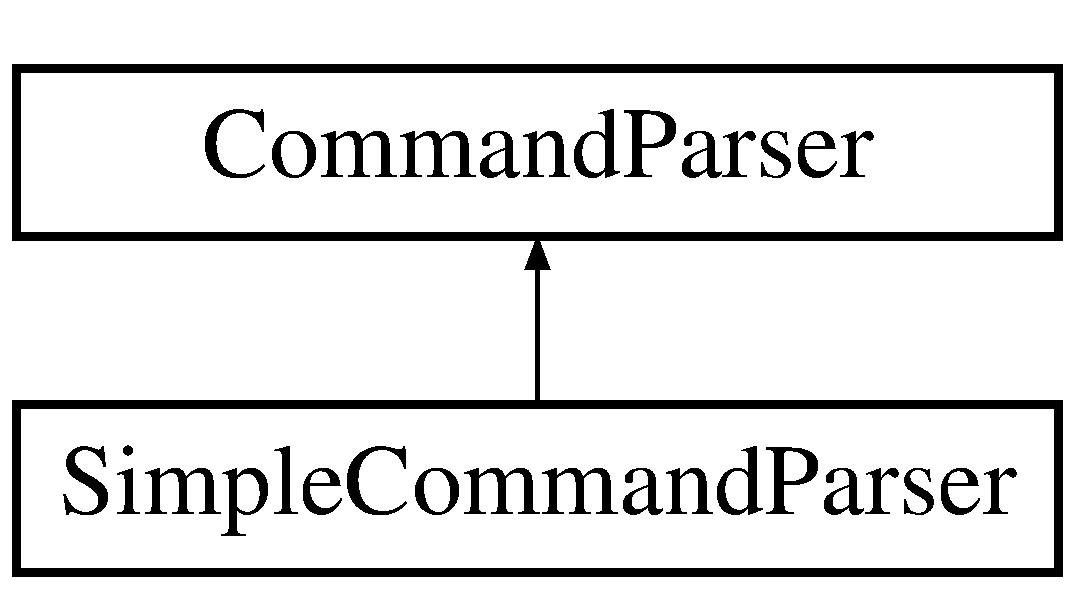
\includegraphics[height=2.000000cm]{class_simple_command_parser}
\end{center}
\end{figure}
\subsection*{Public Member Functions}
\begin{DoxyCompactItemize}
\item 
\hyperlink{class_simple_command_parser_a36f481c3b38076dd51af0b3b21dfc799}{Simple\+Command\+Parser} ()
\item 
\hypertarget{class_simple_command_parser_a62668b9abee69fbbe2abf7e46858691a}{}{\bfseries Simple\+Command\+Parser} (Calculator $\ast$new\+Calculator)\label{class_simple_command_parser_a62668b9abee69fbbe2abf7e46858691a}

\item 
\hypertarget{class_simple_command_parser_a759779af9ad397dcd267b2ac43a43509}{}void {\bfseries set\+Calculator} (Calculator $\ast$new\+Calculator)\label{class_simple_command_parser_a759779af9ad397dcd267b2ac43a43509}

\item 
\hypertarget{class_simple_command_parser_ad852317f775853e0e39f82c26753a0e1}{}void {\bfseries set\+State} (\hyperlink{class_simple_command_parser_state}{Simple\+Command\+Parser\+State} $\ast$new\+State)\label{class_simple_command_parser_ad852317f775853e0e39f82c26753a0e1}

\item 
\hypertarget{class_simple_command_parser_a029433f8b08defadd23ea777b1d7018a}{}void \hyperlink{class_simple_command_parser_a029433f8b08defadd23ea777b1d7018a}{push\+Enter\+Calcul} ()\label{class_simple_command_parser_a029433f8b08defadd23ea777b1d7018a}

\begin{DoxyCompactList}\small\item\em Process calcualtion after pushing button Enter. Hovewer it method used in math sign buttons also. \end{DoxyCompactList}\item 
\hypertarget{class_simple_command_parser_a3cd15cf8330f7da84256e0d5af5055bc}{}void \hyperlink{class_simple_command_parser_a3cd15cf8330f7da84256e0d5af5055bc}{push\+Sign\+Calcul} ()\label{class_simple_command_parser_a3cd15cf8330f7da84256e0d5af5055bc}

\begin{DoxyCompactList}\small\item\em Process calculation after pushing buttons +-\//$\ast$. \end{DoxyCompactList}\item 
\hypertarget{class_simple_command_parser_a2bda6ce2c0a67a245abd22ff77c72b47}{}void {\bfseries do\+Math\+Op\+When\+Enter\+Command} ()\label{class_simple_command_parser_a2bda6ce2c0a67a245abd22ff77c72b47}

\item 
\hypertarget{class_simple_command_parser_a0d0205d4d10998bad63e2c48b7a41054}{}void {\bfseries do\+Math\+Op\+When\+Sign\+Command} ()\label{class_simple_command_parser_a0d0205d4d10998bad63e2c48b7a41054}

\item 
\hypertarget{class_simple_command_parser_aa02939ea765a1086b025862cf8243d34}{}void {\bfseries put\+Result\+To\+Screen} ()\label{class_simple_command_parser_aa02939ea765a1086b025862cf8243d34}

\item 
\hypertarget{class_simple_command_parser_ab89c0661f33a83df7c594e26f508e8ea}{}void {\bfseries add\+Digit\+To\+Digit\+List} ()\label{class_simple_command_parser_ab89c0661f33a83df7c594e26f508e8ea}

\item 
\hypertarget{class_simple_command_parser_a2aa1f98b29f3b6770e86913da8141be4}{}void {\bfseries add\+Digit\+To\+Result\+List} ()\label{class_simple_command_parser_a2aa1f98b29f3b6770e86913da8141be4}

\end{DoxyCompactItemize}
\subsection*{Public Attributes}
\begin{DoxyCompactItemize}
\item 
\hypertarget{class_simple_command_parser_a89b6340ce40c9a4c444876ebdc3d0de2}{}Calculator $\ast$ {\bfseries calculator}\label{class_simple_command_parser_a89b6340ce40c9a4c444876ebdc3d0de2}

\item 
\hypertarget{class_simple_command_parser_a4b66f3e8e15338b02a7f71477d6daa38}{}\hyperlink{class_simple_command_parser_state}{Simple\+Command\+Parser\+State} $\ast$ {\bfseries state\+Parser}\label{class_simple_command_parser_a4b66f3e8e15338b02a7f71477d6daa38}

\end{DoxyCompactItemize}


\subsection{Detailed Description}
Calculator -\/ Simple calculator realization by patterns Copyright (C) 2017 -\/ ? Alexey Konyshev (\href{mailto:aleksey.konyshev@gmail.com}{\tt aleksey.\+konyshev@gmail.\+com})

This software is provided \textquotesingle{}as-\/is\textquotesingle{}, without any express or implied warranty. In no event will the authors be held liable for any damages arising from the use of this software.

Permission is granted to anyone to use this software for any purpose, including commercial applications, and to alter it and redistribute it freely, subject to the following restrictions\+:


\begin{DoxyEnumerate}
\item The origin of this software must not be misrepresented; you must not claim that you wrote the original software. If you use this software in a product, an acknowledgment in the product documentation would be appreciated but is not required.
\item Altered source versions must be plainly marked as such, and must not be misrepresented as being the original software.
\item This notice may not be removed or altered from any source distribution. 
\end{DoxyEnumerate}

\subsection{Constructor \& Destructor Documentation}
\hypertarget{class_simple_command_parser_a36f481c3b38076dd51af0b3b21dfc799}{}\index{Simple\+Command\+Parser@{Simple\+Command\+Parser}!Simple\+Command\+Parser@{Simple\+Command\+Parser}}
\index{Simple\+Command\+Parser@{Simple\+Command\+Parser}!Simple\+Command\+Parser@{Simple\+Command\+Parser}}
\subsubsection[{Simple\+Command\+Parser()}]{\setlength{\rightskip}{0pt plus 5cm}Simple\+Command\+Parser\+::\+Simple\+Command\+Parser (
\begin{DoxyParamCaption}
{}
\end{DoxyParamCaption}
)}\label{class_simple_command_parser_a36f481c3b38076dd51af0b3b21dfc799}
Calculator -\/ Simple calculator realization by patterns Copyright (C) 2017 -\/ ? Alexey Konyshev (\href{mailto:aleksey.konyshev@gmail.com}{\tt aleksey.\+konyshev@gmail.\+com})

This software is provided \textquotesingle{}as-\/is\textquotesingle{}, without any express or implied warranty. In no event will the authors be held liable for any damages arising from the use of this software.

Permission is granted to anyone to use this software for any purpose, including commercial applications, and to alter it and redistribute it freely, subject to the following restrictions\+:


\begin{DoxyEnumerate}
\item The origin of this software must not be misrepresented; you must not claim that you wrote the original software. If you use this software in a product, an acknowledgment in the product documentation would be appreciated but is not required.
\item Altered source versions must be plainly marked as such, and must not be misrepresented as being the original software.
\item This notice may not be removed or altered from any source distribution. 
\end{DoxyEnumerate}

The documentation for this class was generated from the following files\+:\begin{DoxyCompactItemize}
\item 
Simple\+Command\+Parser.\+h\item 
Simple\+Command\+Parser.\+cpp\end{DoxyCompactItemize}

\hypertarget{class_simple_screen}{}\section{Simple\+Screen Class Reference}
\label{class_simple_screen}\index{Simple\+Screen@{Simple\+Screen}}
Inheritance diagram for Simple\+Screen\+:\begin{figure}[H]
\begin{center}
\leavevmode
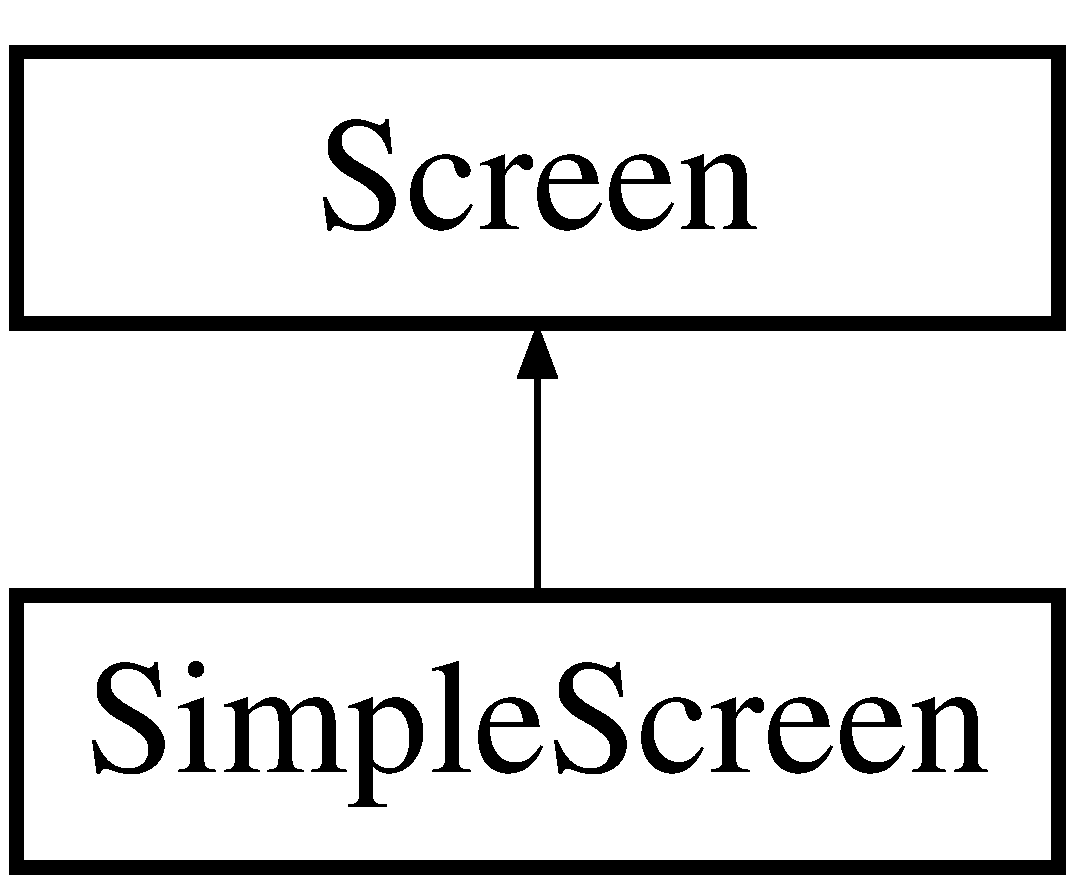
\includegraphics[height=2.000000cm]{class_simple_screen}
\end{center}
\end{figure}
\subsection*{Public Member Functions}
\begin{DoxyCompactItemize}
\item 
\hypertarget{class_simple_screen_af27275c09a784299846ccbabce46db2f}{}\hyperlink{class_simple_screen_af27275c09a784299846ccbabce46db2f}{Simple\+Screen} ()\label{class_simple_screen_af27275c09a784299846ccbabce46db2f}

\begin{DoxyCompactList}\small\item\em Default constructor. \end{DoxyCompactList}\item 
\hypertarget{class_simple_screen_a6cb5a9e1c39a1d5fa6b80a95dc5ec817}{}\hyperlink{class_simple_screen_a6cb5a9e1c39a1d5fa6b80a95dc5ec817}{$\sim$\+Simple\+Screen} ()\label{class_simple_screen_a6cb5a9e1c39a1d5fa6b80a95dc5ec817}

\begin{DoxyCompactList}\small\item\em destructor \end{DoxyCompactList}\end{DoxyCompactItemize}
\subsection*{Additional Inherited Members}


The documentation for this class was generated from the following files\+:\begin{DoxyCompactItemize}
\item 
Simple\+Screen.\+h\item 
Simple\+Screen.\+cpp\end{DoxyCompactItemize}

\hypertarget{class_six_command}{}\section{Six\+Command Class Reference}
\label{class_six_command}\index{Six\+Command@{Six\+Command}}


implementations of six command  




{\ttfamily \#include $<$Six\+Command.\+h$>$}

Inheritance diagram for Six\+Command\+:\begin{figure}[H]
\begin{center}
\leavevmode
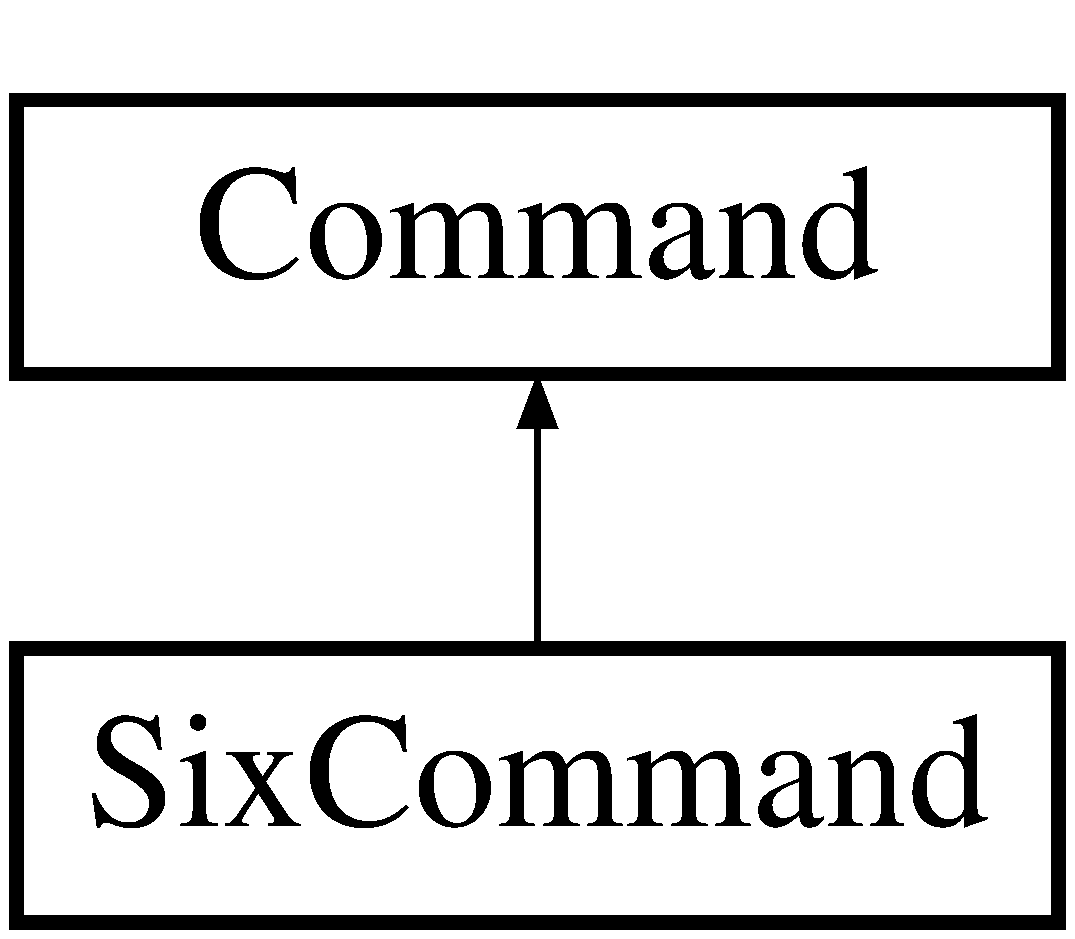
\includegraphics[height=2.000000cm]{class_six_command}
\end{center}
\end{figure}
\subsection*{Public Member Functions}
\begin{DoxyCompactItemize}
\item 
\hyperlink{class_six_command_aed104b7b3d32d680f6459fc7a124c5a3}{Six\+Command} (Calculator $\ast$new\+Calc)
\begin{DoxyCompactList}\small\item\em A constructor. Sets pointer to the implementation of. \end{DoxyCompactList}\item 
\hyperlink{class_six_command_ac2c319c9e53443ff2c4b00a1ccd05c6a}{$\sim$\+Six\+Command} ()
\item 
void \hyperlink{class_six_command_af34a36bfb4cfd411238144e0afce9d28}{execute} ()
\begin{DoxyCompactList}\small\item\em Executes diving command of. \end{DoxyCompactList}\end{DoxyCompactItemize}
\subsection*{Public Attributes}
\begin{DoxyCompactItemize}
\item 
Calculator $\ast$ \hyperlink{class_six_command_aaad9b0fc44a03f98f2de91a140f9a0c2}{calculator}
\end{DoxyCompactItemize}


\subsection{Detailed Description}
implementations of six command 

Calculator -\/ Simple calculator realization by patterns Copyright (C) 2017 -\/ ? Alexey Konyshev (\href{mailto:aleksey.konyshev@gmail.com}{\tt aleksey.\+konyshev@gmail.\+com})

This software is provided \textquotesingle{}as-\/is\textquotesingle{}, without any express or implied warranty. In no event will the authors be held liable for any damages arising from the use of this software.

Permission is granted to anyone to use this software for any purpose, including commercial applications, and to alter it and redistribute it freely, subject to the following restrictions\+:


\begin{DoxyEnumerate}
\item The origin of this software must not be misrepresented; you must not claim that you wrote the original software. If you use this software in a product, an acknowledgment in the product documentation would be appreciated but is not required.
\item Altered source versions must be plainly marked as such, and must not be misrepresented as being the original software.
\item This notice may not be removed or altered from any source distribution. Headers 
\begin{DoxyCode}
\hyperlink{class_command}{Command} 
\end{DoxyCode}
 
\end{DoxyEnumerate}

\subsection{Constructor \& Destructor Documentation}
\hypertarget{class_six_command_aed104b7b3d32d680f6459fc7a124c5a3}{}\index{Six\+Command@{Six\+Command}!Six\+Command@{Six\+Command}}
\index{Six\+Command@{Six\+Command}!Six\+Command@{Six\+Command}}
\subsubsection[{Six\+Command(\+Calculator $\ast$new\+Calc)}]{\setlength{\rightskip}{0pt plus 5cm}Six\+Command\+::\+Six\+Command (
\begin{DoxyParamCaption}
\item[{Calculator $\ast$}]{new\+Calc}
\end{DoxyParamCaption}
)}\label{class_six_command_aed104b7b3d32d680f6459fc7a124c5a3}


A constructor. Sets pointer to the implementation of. 


\begin{DoxyCode}
Calculator 
\end{DoxyCode}



\begin{DoxyParams}{Parameters}
{\em new\+Calc} & a new
\begin{DoxyCode}
Calculator 
\end{DoxyCode}
\\
\hline
\end{DoxyParams}
Calculator -\/ Simple calculator realization by patterns Copyright (C) 2017 -\/ ? Alexey Konyshev (\href{mailto:aleksey.konyshev@gmail.com}{\tt aleksey.\+konyshev@gmail.\+com})

This software is provided \textquotesingle{}as-\/is\textquotesingle{}, without any express or implied warranty. In no event will the authors be held liable for any damages arising from the use of this software.

Permission is granted to anyone to use this software for any purpose, including commercial applications, and to alter it and redistribute it freely, subject to the following restrictions\+:


\begin{DoxyEnumerate}
\item The origin of this software must not be misrepresented; you must not claim that you wrote the original software. If you use this software in a product, an acknowledgment in the product documentation would be appreciated but is not required.
\item Altered source versions must be plainly marked as such, and must not be misrepresented as being the original software.
\item This notice may not be removed or altered from any source distribution. Headers 
\end{DoxyEnumerate}\hypertarget{class_six_command_ac2c319c9e53443ff2c4b00a1ccd05c6a}{}\index{Six\+Command@{Six\+Command}!````~Six\+Command@{$\sim$\+Six\+Command}}
\index{````~Six\+Command@{$\sim$\+Six\+Command}!Six\+Command@{Six\+Command}}
\subsubsection[{$\sim$\+Six\+Command()}]{\setlength{\rightskip}{0pt plus 5cm}Six\+Command\+::$\sim$\+Six\+Command (
\begin{DoxyParamCaption}
{}
\end{DoxyParamCaption}
)}\label{class_six_command_ac2c319c9e53443ff2c4b00a1ccd05c6a}
A destructor 

\subsection{Member Function Documentation}
\hypertarget{class_six_command_af34a36bfb4cfd411238144e0afce9d28}{}\index{Six\+Command@{Six\+Command}!execute@{execute}}
\index{execute@{execute}!Six\+Command@{Six\+Command}}
\subsubsection[{execute()}]{\setlength{\rightskip}{0pt plus 5cm}void Six\+Command\+::execute (
\begin{DoxyParamCaption}
{}
\end{DoxyParamCaption}
)\hspace{0.3cm}{\ttfamily [virtual]}}\label{class_six_command_af34a36bfb4cfd411238144e0afce9d28}


Executes diving command of. 


\begin{DoxyCode}
Calculator 
\end{DoxyCode}
 

Implements \hyperlink{class_command_a6fd7d9bd8df8bfc881e4d6c7cd1878b7}{Command}.



\subsection{Member Data Documentation}
\hypertarget{class_six_command_aaad9b0fc44a03f98f2de91a140f9a0c2}{}\index{Six\+Command@{Six\+Command}!calculator@{calculator}}
\index{calculator@{calculator}!Six\+Command@{Six\+Command}}
\subsubsection[{calculator}]{\setlength{\rightskip}{0pt plus 5cm}Calculator$\ast$ Six\+Command\+::calculator}\label{class_six_command_aaad9b0fc44a03f98f2de91a140f9a0c2}
pointer to the
\begin{DoxyCode}
Calculator 
\end{DoxyCode}
 

The documentation for this class was generated from the following files\+:\begin{DoxyCompactItemize}
\item 
Six\+Command.\+h\item 
Six\+Command.\+cpp\end{DoxyCompactItemize}

\hypertarget{class_str_to_dig}{}\section{Str\+To\+Dig Class Reference}
\label{class_str_to_dig}\index{Str\+To\+Dig@{Str\+To\+Dig}}


{\ttfamily \#include $<$Str\+To\+Dig.\+h$>$}

\subsection*{Public Member Functions}
\begin{DoxyCompactItemize}
\item 
\hyperlink{class_str_to_dig_abdd16d53d16907eeaf6026097c38658f}{Str\+To\+Dig} ()
\item 
\hypertarget{class_str_to_dig_a77478d5ac1f4dca2c1cbecda407fbf56}{}void {\bfseries add\+Digits\+String} (std\+::string dig\+String)\label{class_str_to_dig_a77478d5ac1f4dca2c1cbecda407fbf56}

\item 
\hypertarget{class_str_to_dig_af20b09f86e90d18f83c4c87e6f34cc1e}{}void {\bfseries add\+Digits\+String} (double dig\+Double)\label{class_str_to_dig_af20b09f86e90d18f83c4c87e6f34cc1e}

\item 
\hypertarget{class_str_to_dig_afbb98b1ef5730992ec6fcacf024f575d}{}double {\bfseries get\+Double} ()\label{class_str_to_dig_afbb98b1ef5730992ec6fcacf024f575d}

\item 
\hypertarget{class_str_to_dig_a5a53d889ec55a4be20a6007d0e9df2b6}{}void {\bfseries clear} ()\label{class_str_to_dig_a5a53d889ec55a4be20a6007d0e9df2b6}

\item 
\hypertarget{class_str_to_dig_a3a913de6f12f2773283eaa18c66d5749}{}int {\bfseries get\+Size} ()\label{class_str_to_dig_a3a913de6f12f2773283eaa18c66d5749}

\end{DoxyCompactItemize}
\subsection*{Public Attributes}
\begin{DoxyCompactItemize}
\item 
\hypertarget{class_str_to_dig_aad04956b7e82a5747c5bff326847c361}{}std\+::stringstream {\bfseries ss}\label{class_str_to_dig_aad04956b7e82a5747c5bff326847c361}

\item 
\hypertarget{class_str_to_dig_a8a3a32b98e04f6e418c1218c97b9cf54}{}int {\bfseries size}\label{class_str_to_dig_a8a3a32b98e04f6e418c1218c97b9cf54}

\end{DoxyCompactItemize}


\subsection{Detailed Description}
Calculator -\/ Simple calculator realization by patterns Copyright (C) 2017 -\/ ? Alexey Konyshev (\href{mailto:aleksey.konyshev@gmail.com}{\tt aleksey.\+konyshev@gmail.\+com})

This software is provided \textquotesingle{}as-\/is\textquotesingle{}, without any express or implied warranty. In no event will the authors be held liable for any damages arising from the use of this software.

Permission is granted to anyone to use this software for any purpose, including commercial applications, and to alter it and redistribute it freely, subject to the following restrictions\+:


\begin{DoxyEnumerate}
\item The origin of this software must not be misrepresented; you must not claim that you wrote the original software. If you use this software in a product, an acknowledgment in the product documentation would be appreciated but is not required.
\item Altered source versions must be plainly marked as such, and must not be misrepresented as being the original software.
\item This notice may not be removed or altered from any source distribution. 
\end{DoxyEnumerate}

\subsection{Constructor \& Destructor Documentation}
\hypertarget{class_str_to_dig_abdd16d53d16907eeaf6026097c38658f}{}\index{Str\+To\+Dig@{Str\+To\+Dig}!Str\+To\+Dig@{Str\+To\+Dig}}
\index{Str\+To\+Dig@{Str\+To\+Dig}!Str\+To\+Dig@{Str\+To\+Dig}}
\subsubsection[{Str\+To\+Dig()}]{\setlength{\rightskip}{0pt plus 5cm}Str\+To\+Dig\+::\+Str\+To\+Dig (
\begin{DoxyParamCaption}
{}
\end{DoxyParamCaption}
)}\label{class_str_to_dig_abdd16d53d16907eeaf6026097c38658f}
Calculator -\/ Simple calculator realization by patterns Copyright (C) 2017 -\/ ? Alexey Konyshev (\href{mailto:aleksey.konyshev@gmail.com}{\tt aleksey.\+konyshev@gmail.\+com})

This software is provided \textquotesingle{}as-\/is\textquotesingle{}, without any express or implied warranty. In no event will the authors be held liable for any damages arising from the use of this software.

Permission is granted to anyone to use this software for any purpose, including commercial applications, and to alter it and redistribute it freely, subject to the following restrictions\+:


\begin{DoxyEnumerate}
\item The origin of this software must not be misrepresented; you must not claim that you wrote the original software. If you use this software in a product, an acknowledgment in the product documentation would be appreciated but is not required.
\item Altered source versions must be plainly marked as such, and must not be misrepresented as being the original software.
\item This notice may not be removed or altered from any source distribution. 
\end{DoxyEnumerate}

The documentation for this class was generated from the following files\+:\begin{DoxyCompactItemize}
\item 
Str\+To\+Dig.\+h\item 
Str\+To\+Dig.\+cpp\end{DoxyCompactItemize}

\hypertarget{class_three_command}{}\section{Three\+Command Class Reference}
\label{class_three_command}\index{Three\+Command@{Three\+Command}}


implementations of three command  




{\ttfamily \#include $<$Three\+Command.\+h$>$}

Inheritance diagram for Three\+Command\+:\begin{figure}[H]
\begin{center}
\leavevmode
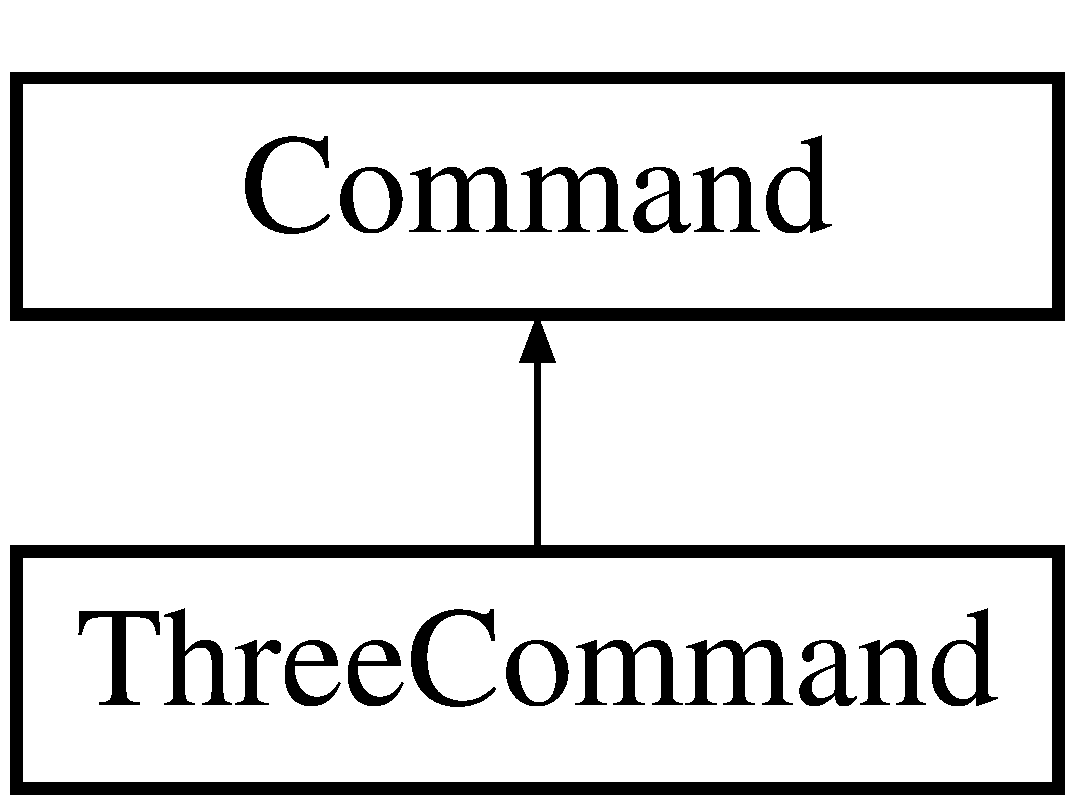
\includegraphics[height=2.000000cm]{class_three_command}
\end{center}
\end{figure}
\subsection*{Public Member Functions}
\begin{DoxyCompactItemize}
\item 
\hyperlink{class_three_command_a6d1887ffb18cd3772b9164d68e86b72c}{Three\+Command} (Calculator $\ast$new\+Calc)
\begin{DoxyCompactList}\small\item\em A constructor. Sets pointer to the implementation of. \end{DoxyCompactList}\item 
\hyperlink{class_three_command_a2d1d9c12174c3b40105ba216a0465033}{$\sim$\+Three\+Command} ()
\item 
void \hyperlink{class_three_command_af8e301161be213f999f4fd49ffa4db67}{execute} ()
\begin{DoxyCompactList}\small\item\em Executes three command of. \end{DoxyCompactList}\end{DoxyCompactItemize}
\subsection*{Public Attributes}
\begin{DoxyCompactItemize}
\item 
Calculator $\ast$ \hyperlink{class_three_command_a8a2a28c69c47a9e7d65a0b487c41596a}{calculator}
\end{DoxyCompactItemize}


\subsection{Detailed Description}
implementations of three command 

Calculator -\/ Simple calculator realization by patterns Copyright (C) 2017 -\/ ? Alexey Konyshev (\href{mailto:aleksey.konyshev@gmail.com}{\tt aleksey.\+konyshev@gmail.\+com})

This software is provided \textquotesingle{}as-\/is\textquotesingle{}, without any express or implied warranty. In no event will the authors be held liable for any damages arising from the use of this software.

Permission is granted to anyone to use this software for any purpose, including commercial applications, and to alter it and redistribute it freely, subject to the following restrictions\+:


\begin{DoxyEnumerate}
\item The origin of this software must not be misrepresented; you must not claim that you wrote the original software. If you use this software in a product, an acknowledgment in the product documentation would be appreciated but is not required.
\item Altered source versions must be plainly marked as such, and must not be misrepresented as being the original software.
\item This notice may not be removed or altered from any source distribution. Headers 
\begin{DoxyCode}
\hyperlink{class_command}{Command} 
\end{DoxyCode}
 
\end{DoxyEnumerate}

\subsection{Constructor \& Destructor Documentation}
\hypertarget{class_three_command_a6d1887ffb18cd3772b9164d68e86b72c}{}\index{Three\+Command@{Three\+Command}!Three\+Command@{Three\+Command}}
\index{Three\+Command@{Three\+Command}!Three\+Command@{Three\+Command}}
\subsubsection[{Three\+Command(\+Calculator $\ast$new\+Calc)}]{\setlength{\rightskip}{0pt plus 5cm}Three\+Command\+::\+Three\+Command (
\begin{DoxyParamCaption}
\item[{Calculator $\ast$}]{new\+Calc}
\end{DoxyParamCaption}
)}\label{class_three_command_a6d1887ffb18cd3772b9164d68e86b72c}


A constructor. Sets pointer to the implementation of. 


\begin{DoxyCode}
Calculator 
\end{DoxyCode}



\begin{DoxyParams}{Parameters}
{\em new\+Calc} & a new
\begin{DoxyCode}
Calculator 
\end{DoxyCode}
\\
\hline
\end{DoxyParams}
Calculator -\/ Simple calculator realization by patterns Copyright (C) 2017 -\/ ? Alexey Konyshev (\href{mailto:aleksey.konyshev@gmail.com}{\tt aleksey.\+konyshev@gmail.\+com})

This software is provided \textquotesingle{}as-\/is\textquotesingle{}, without any express or implied warranty. In no event will the authors be held liable for any damages arising from the use of this software.

Permission is granted to anyone to use this software for any purpose, including commercial applications, and to alter it and redistribute it freely, subject to the following restrictions\+:


\begin{DoxyEnumerate}
\item The origin of this software must not be misrepresented; you must not claim that you wrote the original software. If you use this software in a product, an acknowledgment in the product documentation would be appreciated but is not required.
\item Altered source versions must be plainly marked as such, and must not be misrepresented as being the original software.
\item This notice may not be removed or altered from any source distribution. Headers 
\end{DoxyEnumerate}\hypertarget{class_three_command_a2d1d9c12174c3b40105ba216a0465033}{}\index{Three\+Command@{Three\+Command}!````~Three\+Command@{$\sim$\+Three\+Command}}
\index{````~Three\+Command@{$\sim$\+Three\+Command}!Three\+Command@{Three\+Command}}
\subsubsection[{$\sim$\+Three\+Command()}]{\setlength{\rightskip}{0pt plus 5cm}Three\+Command\+::$\sim$\+Three\+Command (
\begin{DoxyParamCaption}
{}
\end{DoxyParamCaption}
)}\label{class_three_command_a2d1d9c12174c3b40105ba216a0465033}
A destructor 

\subsection{Member Function Documentation}
\hypertarget{class_three_command_af8e301161be213f999f4fd49ffa4db67}{}\index{Three\+Command@{Three\+Command}!execute@{execute}}
\index{execute@{execute}!Three\+Command@{Three\+Command}}
\subsubsection[{execute()}]{\setlength{\rightskip}{0pt plus 5cm}void Three\+Command\+::execute (
\begin{DoxyParamCaption}
{}
\end{DoxyParamCaption}
)\hspace{0.3cm}{\ttfamily [virtual]}}\label{class_three_command_af8e301161be213f999f4fd49ffa4db67}


Executes three command of. 


\begin{DoxyCode}
Calculator 
\end{DoxyCode}
 

Implements \hyperlink{class_command_a6fd7d9bd8df8bfc881e4d6c7cd1878b7}{Command}.



\subsection{Member Data Documentation}
\hypertarget{class_three_command_a8a2a28c69c47a9e7d65a0b487c41596a}{}\index{Three\+Command@{Three\+Command}!calculator@{calculator}}
\index{calculator@{calculator}!Three\+Command@{Three\+Command}}
\subsubsection[{calculator}]{\setlength{\rightskip}{0pt plus 5cm}Calculator$\ast$ Three\+Command\+::calculator}\label{class_three_command_a8a2a28c69c47a9e7d65a0b487c41596a}
pointer to the
\begin{DoxyCode}
Calculator 
\end{DoxyCode}
 

The documentation for this class was generated from the following files\+:\begin{DoxyCompactItemize}
\item 
Three\+Command.\+h\item 
Three\+Command.\+cpp\end{DoxyCompactItemize}

\hypertarget{class_two_command}{}\section{Two\+Command Class Reference}
\label{class_two_command}\index{Two\+Command@{Two\+Command}}


implementations of two command  




{\ttfamily \#include $<$Two\+Command.\+h$>$}

Inheritance diagram for Two\+Command\+:\begin{figure}[H]
\begin{center}
\leavevmode
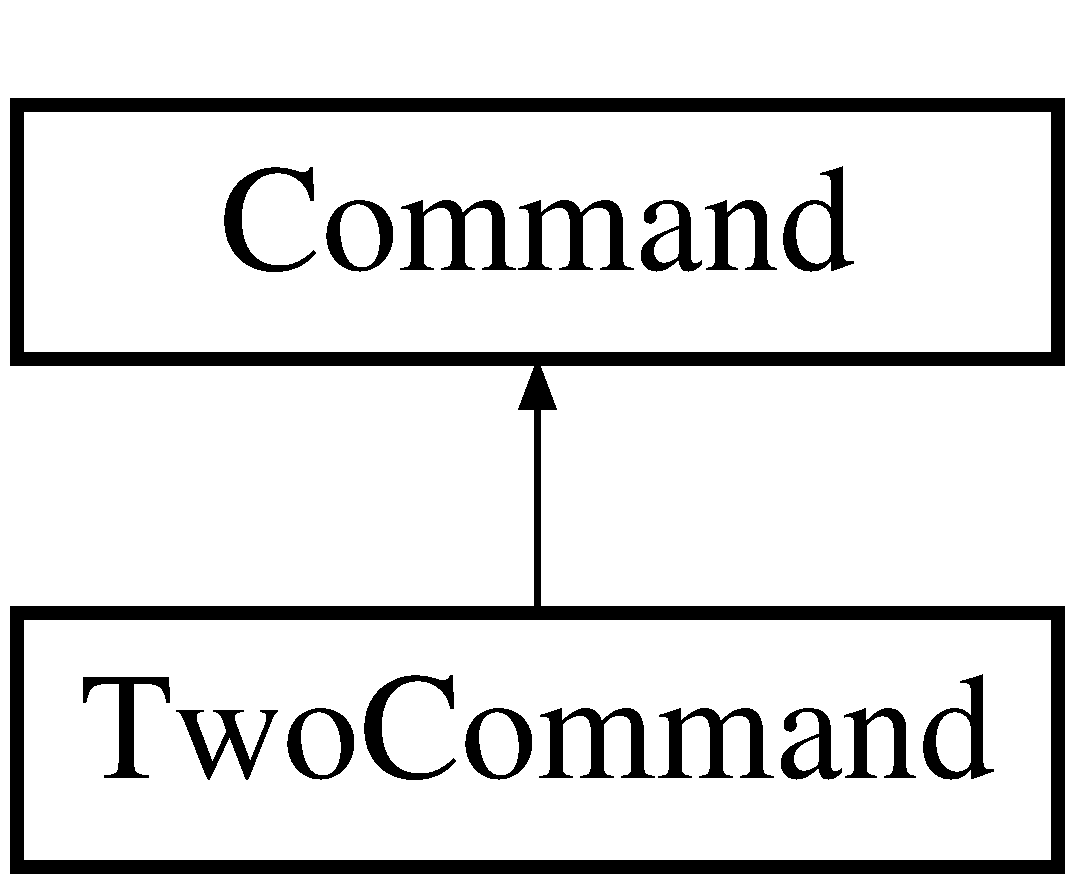
\includegraphics[height=2.000000cm]{class_two_command}
\end{center}
\end{figure}
\subsection*{Public Member Functions}
\begin{DoxyCompactItemize}
\item 
\hyperlink{class_two_command_a73335d14fe98bc82ef181647b5541aea}{Two\+Command} (Calculator $\ast$new\+Calc)
\begin{DoxyCompactList}\small\item\em A constructor. Sets pointer to the implementation of. \end{DoxyCompactList}\item 
\hyperlink{class_two_command_afbb4f51e3f13eba41b80919307015725}{$\sim$\+Two\+Command} ()
\item 
void \hyperlink{class_two_command_a5065cc2a07c69dcba178c82d7610e29f}{execute} ()
\begin{DoxyCompactList}\small\item\em Executes zero command of. \end{DoxyCompactList}\end{DoxyCompactItemize}
\subsection*{Public Attributes}
\begin{DoxyCompactItemize}
\item 
Calculator $\ast$ \hyperlink{class_two_command_a0242384aa6f8091cc5c413d4e4763cf9}{calculator}
\end{DoxyCompactItemize}


\subsection{Detailed Description}
implementations of two command 

Calculator -\/ Simple calculator realization by patterns Copyright (C) 2017 -\/ ? Alexey Konyshev (\href{mailto:aleksey.konyshev@gmail.com}{\tt aleksey.\+konyshev@gmail.\+com})

This software is provided \textquotesingle{}as-\/is\textquotesingle{}, without any express or implied warranty. In no event will the authors be held liable for any damages arising from the use of this software.

Permission is granted to anyone to use this software for any purpose, including commercial applications, and to alter it and redistribute it freely, subject to the following restrictions\+:


\begin{DoxyEnumerate}
\item The origin of this software must not be misrepresented; you must not claim that you wrote the original software. If you use this software in a product, an acknowledgment in the product documentation would be appreciated but is not required.
\item Altered source versions must be plainly marked as such, and must not be misrepresented as being the original software.
\item This notice may not be removed or altered from any source distribution. Headers 
\begin{DoxyCode}
\hyperlink{class_command}{Command} 
\end{DoxyCode}
 
\end{DoxyEnumerate}

\subsection{Constructor \& Destructor Documentation}
\hypertarget{class_two_command_a73335d14fe98bc82ef181647b5541aea}{}\index{Two\+Command@{Two\+Command}!Two\+Command@{Two\+Command}}
\index{Two\+Command@{Two\+Command}!Two\+Command@{Two\+Command}}
\subsubsection[{Two\+Command(\+Calculator $\ast$new\+Calc)}]{\setlength{\rightskip}{0pt plus 5cm}Two\+Command\+::\+Two\+Command (
\begin{DoxyParamCaption}
\item[{Calculator $\ast$}]{new\+Calc}
\end{DoxyParamCaption}
)}\label{class_two_command_a73335d14fe98bc82ef181647b5541aea}


A constructor. Sets pointer to the implementation of. 


\begin{DoxyCode}
Calculator 
\end{DoxyCode}



\begin{DoxyParams}{Parameters}
{\em new\+Calc} & a new
\begin{DoxyCode}
Calculator 
\end{DoxyCode}
\\
\hline
\end{DoxyParams}
Calculator -\/ Simple calculator realization by patterns Copyright (C) 2017 -\/ ? Alexey Konyshev (\href{mailto:aleksey.konyshev@gmail.com}{\tt aleksey.\+konyshev@gmail.\+com})

This software is provided \textquotesingle{}as-\/is\textquotesingle{}, without any express or implied warranty. In no event will the authors be held liable for any damages arising from the use of this software.

Permission is granted to anyone to use this software for any purpose, including commercial applications, and to alter it and redistribute it freely, subject to the following restrictions\+:


\begin{DoxyEnumerate}
\item The origin of this software must not be misrepresented; you must not claim that you wrote the original software. If you use this software in a product, an acknowledgment in the product documentation would be appreciated but is not required.
\item Altered source versions must be plainly marked as such, and must not be misrepresented as being the original software.
\item This notice may not be removed or altered from any source distribution. Headers 
\end{DoxyEnumerate}\hypertarget{class_two_command_afbb4f51e3f13eba41b80919307015725}{}\index{Two\+Command@{Two\+Command}!````~Two\+Command@{$\sim$\+Two\+Command}}
\index{````~Two\+Command@{$\sim$\+Two\+Command}!Two\+Command@{Two\+Command}}
\subsubsection[{$\sim$\+Two\+Command()}]{\setlength{\rightskip}{0pt plus 5cm}Two\+Command\+::$\sim$\+Two\+Command (
\begin{DoxyParamCaption}
{}
\end{DoxyParamCaption}
)}\label{class_two_command_afbb4f51e3f13eba41b80919307015725}
A destructor 

\subsection{Member Function Documentation}
\hypertarget{class_two_command_a5065cc2a07c69dcba178c82d7610e29f}{}\index{Two\+Command@{Two\+Command}!execute@{execute}}
\index{execute@{execute}!Two\+Command@{Two\+Command}}
\subsubsection[{execute()}]{\setlength{\rightskip}{0pt plus 5cm}void Two\+Command\+::execute (
\begin{DoxyParamCaption}
{}
\end{DoxyParamCaption}
)\hspace{0.3cm}{\ttfamily [virtual]}}\label{class_two_command_a5065cc2a07c69dcba178c82d7610e29f}


Executes zero command of. 


\begin{DoxyCode}
Calculator 
\end{DoxyCode}
 

Implements \hyperlink{class_command_a6fd7d9bd8df8bfc881e4d6c7cd1878b7}{Command}.



\subsection{Member Data Documentation}
\hypertarget{class_two_command_a0242384aa6f8091cc5c413d4e4763cf9}{}\index{Two\+Command@{Two\+Command}!calculator@{calculator}}
\index{calculator@{calculator}!Two\+Command@{Two\+Command}}
\subsubsection[{calculator}]{\setlength{\rightskip}{0pt plus 5cm}Calculator$\ast$ Two\+Command\+::calculator}\label{class_two_command_a0242384aa6f8091cc5c413d4e4763cf9}
pointer to the
\begin{DoxyCode}
Calculator 
\end{DoxyCode}
 

The documentation for this class was generated from the following files\+:\begin{DoxyCompactItemize}
\item 
Two\+Command.\+h\item 
Two\+Command.\+cpp\end{DoxyCompactItemize}

\hypertarget{class_waiting_screen_state}{}\section{Waiting\+Screen\+State Class Reference}
\label{class_waiting_screen_state}\index{Waiting\+Screen\+State@{Waiting\+Screen\+State}}


Implementations of.  




{\ttfamily \#include $<$Waiting\+Screen\+State.\+h$>$}

Inheritance diagram for Waiting\+Screen\+State\+:\begin{figure}[H]
\begin{center}
\leavevmode
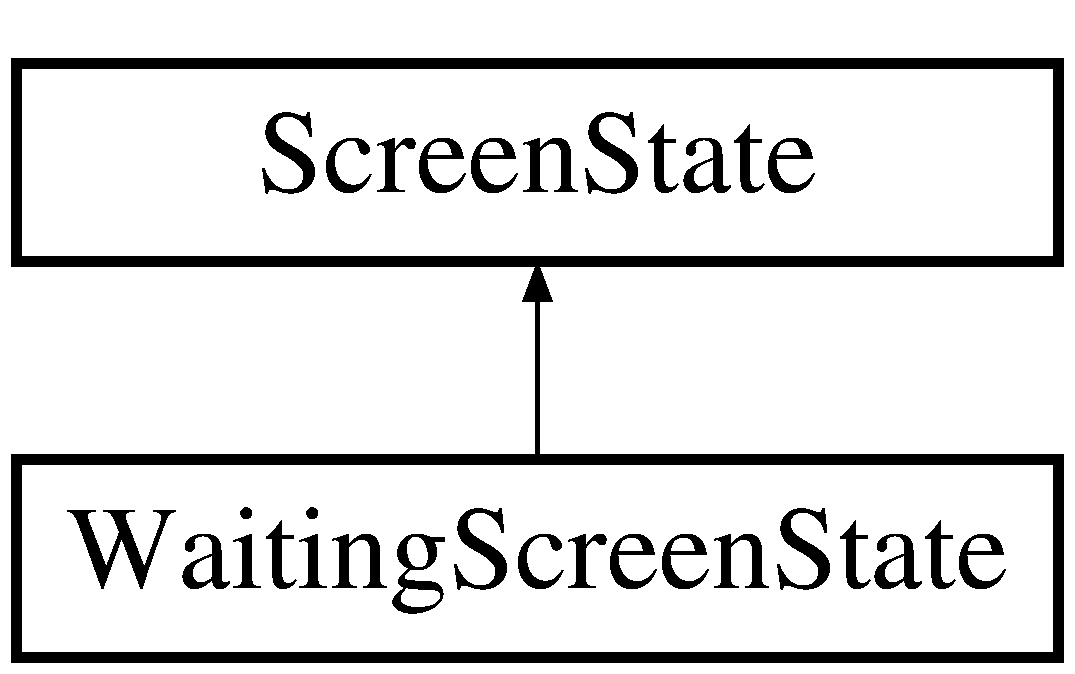
\includegraphics[height=2.000000cm]{class_waiting_screen_state}
\end{center}
\end{figure}
\subsection*{Public Member Functions}
\begin{DoxyCompactItemize}
\item 
void \hyperlink{class_waiting_screen_state_a35c29d113f4110d165fffdfe6ef1a57c}{set\+Screen} (\hyperlink{class_screen}{Screen} $\ast$new\+Screan)
\begin{DoxyCompactList}\small\item\em Set new screen. \end{DoxyCompactList}\item 
void \hyperlink{class_waiting_screen_state_ac22e314bd11df4ba4d5480da022f5862}{input} (std\+::string new\+Symbol)
\begin{DoxyCompactList}\small\item\em Input new symbol to the screan according current state. \end{DoxyCompactList}\item 
\hypertarget{class_waiting_screen_state_aa411b1a427f9a112ddaaff80105bbaff}{}void \hyperlink{class_waiting_screen_state_aa411b1a427f9a112ddaaff80105bbaff}{clear} ()\label{class_waiting_screen_state_aa411b1a427f9a112ddaaff80105bbaff}

\begin{DoxyCompactList}\small\item\em Clear screen according state. \end{DoxyCompactList}\end{DoxyCompactItemize}
\subsection*{Static Public Member Functions}
\begin{DoxyCompactItemize}
\item 
\hypertarget{class_waiting_screen_state_a0bba467dd415c8e5cadc5acaee5f64f5}{}static \hyperlink{class_waiting_screen_state}{Waiting\+Screen\+State} \& {\bfseries Instance} ()\label{class_waiting_screen_state_a0bba467dd415c8e5cadc5acaee5f64f5}

\end{DoxyCompactItemize}
\subsection*{Public Attributes}
\begin{DoxyCompactItemize}
\item 
\hypertarget{class_waiting_screen_state_ad10a8cdba52398cf2043ebe6f83b67ee}{}\hyperlink{class_screen}{Screen} $\ast$ {\bfseries screen}\label{class_waiting_screen_state_ad10a8cdba52398cf2043ebe6f83b67ee}

\end{DoxyCompactItemize}


\subsection{Detailed Description}
Implementations of. 


\begin{DoxyCode}
\hyperlink{class_screen_state}{ScreenState} 
\end{DoxyCode}
 . The class designed as Singletone we must be shue before using the state class that link to
\begin{DoxyCode}
\hyperlink{class_screen}{Screen} 
\end{DoxyCode}
 is not N\+U\+L\+L so where we initialize the programm we set to states link to the
\begin{DoxyCode}
\hyperlink{class_screen}{Screen} 
\end{DoxyCode}
 and can use everywhere state classes 

\subsection{Member Function Documentation}
\hypertarget{class_waiting_screen_state_ac22e314bd11df4ba4d5480da022f5862}{}\index{Waiting\+Screen\+State@{Waiting\+Screen\+State}!input@{input}}
\index{input@{input}!Waiting\+Screen\+State@{Waiting\+Screen\+State}}
\subsubsection[{input(std\+::string new\+Symbol)}]{\setlength{\rightskip}{0pt plus 5cm}void Waiting\+Screen\+State\+::input (
\begin{DoxyParamCaption}
\item[{std\+::string}]{new\+Symbol}
\end{DoxyParamCaption}
)\hspace{0.3cm}{\ttfamily [virtual]}}\label{class_waiting_screen_state_ac22e314bd11df4ba4d5480da022f5862}


Input new symbol to the screan according current state. 


\begin{DoxyParams}{Parameters}
{\em new\+Symbol} & \\
\hline
\end{DoxyParams}


Implements \hyperlink{class_screen_state_adb71081141ec6c066d54f1dc77c78717}{Screen\+State}.

\hypertarget{class_waiting_screen_state_a35c29d113f4110d165fffdfe6ef1a57c}{}\index{Waiting\+Screen\+State@{Waiting\+Screen\+State}!set\+Screen@{set\+Screen}}
\index{set\+Screen@{set\+Screen}!Waiting\+Screen\+State@{Waiting\+Screen\+State}}
\subsubsection[{set\+Screen(\+Screen $\ast$new\+Screan)}]{\setlength{\rightskip}{0pt plus 5cm}void Waiting\+Screen\+State\+::set\+Screen (
\begin{DoxyParamCaption}
\item[{{\bf Screen} $\ast$}]{new\+Screan}
\end{DoxyParamCaption}
)}\label{class_waiting_screen_state_a35c29d113f4110d165fffdfe6ef1a57c}


Set new screen. 


\begin{DoxyParams}{Parameters}
{\em new\+Screen} & \mbox{[}description\mbox{]} \\
\hline
\end{DoxyParams}


The documentation for this class was generated from the following files\+:\begin{DoxyCompactItemize}
\item 
Waiting\+Screen\+State.\+h\item 
Waiting\+Screen\+State.\+cpp\end{DoxyCompactItemize}

\hypertarget{class_zero_command}{}\section{Zero\+Command Class Reference}
\label{class_zero_command}\index{Zero\+Command@{Zero\+Command}}
Inheritance diagram for Zero\+Command\+:\begin{figure}[H]
\begin{center}
\leavevmode
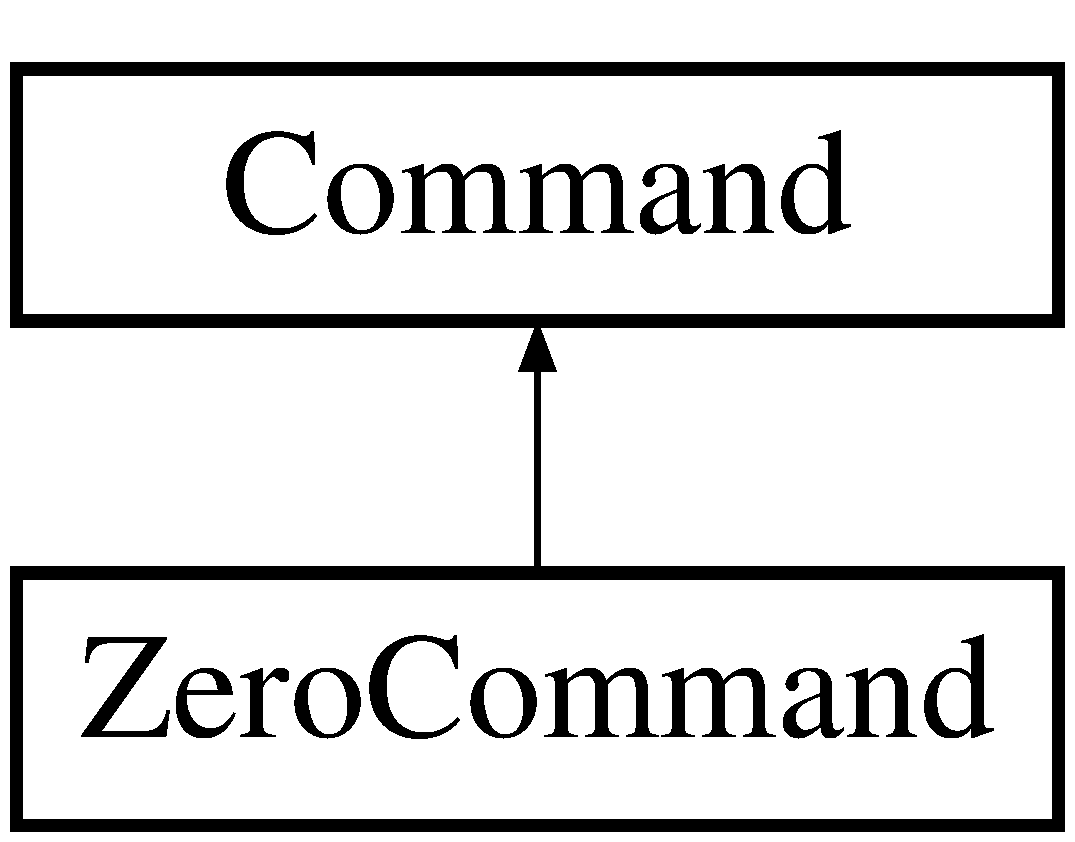
\includegraphics[height=2.000000cm]{class_zero_command}
\end{center}
\end{figure}
\subsection*{Public Member Functions}
\begin{DoxyCompactItemize}
\item 
\hypertarget{class_zero_command_aead23519dff0be47aaab54ebc6f6a2cf}{}{\bfseries Zero\+Command} (\hyperlink{class_calculator}{Calculator} $\ast$new\+Calc)\label{class_zero_command_aead23519dff0be47aaab54ebc6f6a2cf}

\item 
\hypertarget{class_zero_command_ad36f2d99253252274f1bfaa3c5d81c7b}{}void \hyperlink{class_zero_command_ad36f2d99253252274f1bfaa3c5d81c7b}{execute} ()\label{class_zero_command_ad36f2d99253252274f1bfaa3c5d81c7b}

\begin{DoxyCompactList}\small\item\em Executes some functionality in buisness logic. \end{DoxyCompactList}\end{DoxyCompactItemize}
\subsection*{Public Attributes}
\begin{DoxyCompactItemize}
\item 
\hypertarget{class_zero_command_ad478b56405cd23b5c4a597a0c320bef0}{}\hyperlink{class_calculator}{Calculator} $\ast$ {\bfseries calculator}\label{class_zero_command_ad478b56405cd23b5c4a597a0c320bef0}

\end{DoxyCompactItemize}


The documentation for this class was generated from the following files\+:\begin{DoxyCompactItemize}
\item 
Zero\+Command.\+h\item 
Zero\+Command.\+cpp\end{DoxyCompactItemize}

%--- End generated contents ---

% Index
\backmatter
\newpage
\phantomsection
\clearemptydoublepage
\addcontentsline{toc}{chapter}{Index}
\printindex

\end{document}
